\ifnum\aluno=1
\renewcommand\chapterillustration{./abertura-trigonometrica}
\else
\renewcommand\chapterillustration{./abertura-trigonometrica-professor}
\fi


\def\chapterwhat{Fenômenos Periódicos, Radiano, Funções Seno e Cosseno, Senóides.}
\def\chapterbecause{Fenômenos periódicos são aqueles que se repetem com o tempo. Alguns exemplos de tais fenômenos são os batimentos cardíacos, as fases da lua, do nascer do sol, o movimento dos ponteiros de um relógio ou de um pêndulo. O próprio movimento de rotação da Terra é um fenômeno periódico que se repete em períodos de 24 horas, sendo o responsável pelas noções de dia e de noite. As funções trigonométricas, diferente das demais que estudamos até aqui, têm a propriedade de serem periódicas, isto é, seus gráficos se replicam ciclicamente em intervalos determinados do seu domínio. Esta característica faz dessas funções as mais adequadas para modelar matematicamente e prever informações sobre os fenômenos periódicos.} 
\chapter{Funções Trigonométricas}
\label{trigo-chap}

\mbox{}\thispagestyle{empty}\clearpage

\thispagestyle{empty}

\begin{center}
Projeto: LIVRO ABERTO DE MATEMÁTICA

\noindent \begin{tabular}{lcccr}

\includegraphics[scale=.15]{impa}& \quad\quad& 
\includegraphics[width=3cm]{logo} & \quad\quad& 
\includegraphics[scale=.24]{obmep} 
\end{tabular}
\end{center}

\vspace*{.3cm}

Cadastre-se como colaborador no site do projeto: \url{umlivroaberto.org}



% \begin{center}
%   \includegraphics[width=2cm]{canvas}
% \end{center}

\begin{tabular}{p{.15\textwidth}p{.7\textwidth}}
Título: & Funções Trigonométricas\\
\\
Ano/ Versão: & 2020 / versão 0.2 de 17 de novembro de 2020\\
\\
Editora & Instituto Nacional de Matem\'atica Pura e Aplicada (IMPA-OS)\\
\\
Realização:& Olimp\'iada Brasileira de Matem\'atica das Escolas P\'ublicas (OBMEP)\\
\\
Produção:& Associação Livro Aberto\\
\\
Coordenação: & Fabio Simas, \\
			&  Augusto Teixeira (livroaberto@impa.br)\\
\\
  Autor: & Ivail Muniz Junior\\
        
\\
Colaboração: & \\
\\
Revisor: & Amarildo Melchiades da Silva \\
         & Vanessa Matos \\
\\
Design: & Andreza Moreira (Tangentes Design) \\
\\
  Ilustrações: & --- \\ 
\\
Gráficos: & Tarso Caldas (Licenciando da UNIRIO)\\
\\
  Capa: & Foto de Josh Appel, no Unsplash \\
  		& https://unsplash.com/photos/QSipy5RFcSA \\

\end{tabular}
\vspace{.5cm}



\begin{figure}[b]
\begin{minipage}[l]{5cm}
\centering

{\large Licença:}

  
\includegraphics[width=3.5cm]{cc-by-nc-sa}
\end{minipage}\hfill
\begin{minipage}[c]{5cm}
\centering
{\large Desenvolvido por}


\includegraphics[width=2.5cm]{logo-associacao.jpg}
\end{minipage}
\begin{minipage}[r]{5cm}
\centering

{\large Patrocínio:}
  \vspace{1em}
  
\includegraphics[width=3.5cm]{itau}
\end{minipage}
\end{figure}

\mainmatter

\begin{apresentacao}{Introdução}

O conteúdo matemático relacionado a esse capítulo é o das funções trigonométricas. O estudo da Trigonometria tradicionalmente tem um espaço considerável dentro do currículo de matemática do Ensino Médio, se prolongando na maioria das escolas por quase todo um ano letivo. A importância desse tópico se deve tanto à importância teórica dentro da área de Matemática quanto às suas aplicações a outras áreas.

Historicamente, a Trigonometria teve início na antiguidade, quando era utilizada para calcular distâncias e ângulos através do tradicional problema da resolução de triângulos, que consiste em determinar a medida de todos os lados e ângulos desse tipo de figura \citep{Lima2006}.

O problema de utilizar senos e cossenos para calcular medidas dos lados em um triângulo é explorada no último ano do Ensino Fundamental, momento em que estes conceitos são definidos como razões entre catetos e a hipotenusa de um triângulo retângulo. A princípio, essas razões trigonométricas estão restritas a ângulos agudos, pouco depois, a definição cosseno é estendida de maneira natural para ângulos obtusos, numa forma de generalizar o Teorema de Pitágoras para triângulos quaisquer, concretizada pela Lei dos Cossenos. A definição de seno de um ângulo também é estendida para ângulos obtusos, permitindo-se estabelecer a fórmula da Lei dos Senos.

A Trigonometria do triângulo retângulo é resgatada nos primeiros anos do Ensino Médio e a partir daí, muitas mudanças são realizadas na abordagem e nos cálculos de senos e cossenos. Uma delas é a “troca”{} ocorrida na figura central utilizada para realizar esses cálculos, passando do triângulo retângulo para o círculo trigonométrico. Enquanto no Ensino Fundamental, o cálculo das razões trigonométricas se restringia a ângulos agudos ou obtusos medidos em graus, no Ensino Médio, seno e cosseno passam a ser vistos como funções, calculados em números reais. Estabelece-se por fim, a construção de gráficos para essas funções trigonométricas, cristalizando uma interseção sem volta com a área de Álgebra.  

Certamente, algumas das perguntas mais relevantes que, tanto professores de Matemática como alunos que concluem o Ensino Médio deveriam compreender suas respostas é: por que não restringimos os estudos do seno e do cosseno apenas aos triângulos retângulos? Por que há essa necessidade de se trabalhar com ângulos quaisquer no círculo, e mais abstratamente, com cálculo de seno e cosseno de um número real? A resposta a essas perguntas se deve ao fato de que as funções trigonométricas são as mais apropriadas para se modelar os chamados fenômenos de natureza periódica, oscilatória ou vibratória, como o movimento de um pêndulo, o som, as fases da lua, o nível das marés, dentre muitos outros \citep{Lima2006}. De fato, o matemático Joseph Fourier descobriu em 1822 que essencialmente todo fenômeno periódico pode ser modelado por uma soma (que pode ser infinita!) de funções trigonométricas do tipo $a\cos(kx)+b\sen(kx)$.

Como pode-se ver, a Trigonometria é muito vasta, sendo uma das primeiras áreas de estudo em Matemática a conectar Geometria, Álgebra e a Construção de Gráficos, um importante precursor do Cálculo Diferencial e com diferentes aplicações em áreas como Física Newtoniana, Arquitetura e Engenharias \citep{weber2005}. Em particular, destacamos a abstração necessária para realizar a transposição do conceito de seno de ângulos para um número real qualquer. No trabalho de \cite{orhun2010}, percebeu-se que os alunos tinham dificuldade em compreender que os ângulos em radianos expressam um número real e que as funções trigonométricas são funções de números reais em números reais.


\begin{figure}[H]
\centering

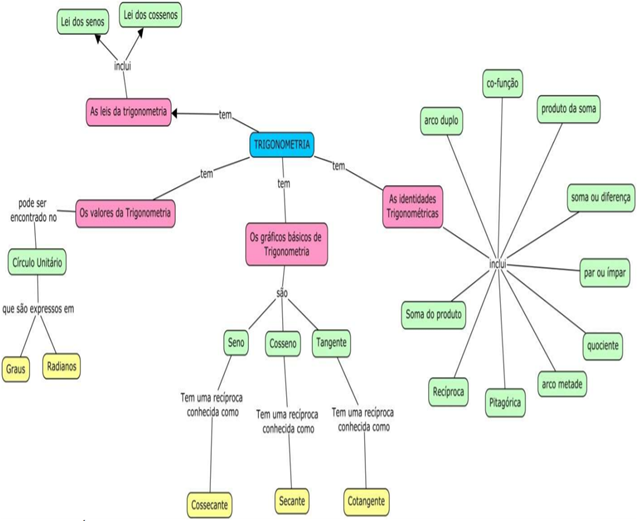
\includegraphics[width=.95\linewidth]{trigonometricas-professor1}
\end{figure}

O mapa conceitual acima ilustra a gama de tópicos que costumam permear o ensino da Trigonometria no Ensino Médio, um verdadeiro desafio para o professor, que busca garantir aos alunos tanto a aprendizagem conceitual de seno, cosseno, radiano, dentre outros elementos como o traquejo no cálculo e no uso de identidades e fórmulas. Dependendo do item estudado, muda-se consideravelmente os objetos geométricos e a linguagem empregados: no item “As Leis da Trigonometria”, os principais resultados se desenvolvem no universo dos ângulos e triângulos. No tópico “os valores da Trigonometria”{} os triângulos perdem o protagonismo e dão lugar ao círculo unitário, assim como os ângulos dão lugar aos arcos. No item “Os gráficos básicos da Trigonometria”, os objetos geométricos que passam a receber ênfase são os gráficos das funções trigonométricas, calculadas não em ângulos ou arcos, mais em números reais. Por fim, os tópicos associados ao item “As identidades trigonométricas”{} podem ser desenvolvidos de forma puramente algébrica. Conexões entre esses itens são necessárias para uma compreensão conceitual adequada da Trigonometria, porém elas podem ficar comprometidas, tendo em vista o grau de diversidade simbólica envolvida, o volume de conteúdo e o tempo do qual o professor dispõe para ministrar suas aulas. Uma possível consequência negativa de um ensino acelerado da Trigonometria seja encontrar com bastante frequência alunos do Ensino Médio ou dos primeiros períodos de cursos de graduação utilizando “macetes”{} para efetuar cálculos envolvendo seno e cosseno. Na imagem abaixo, vemos um dos mais conhecidos, para o cálculo das razões trigonométricas nos ângulos notáveis $30^{\circ}$, $45^{\circ}$ e $60^{\circ}$.


\begin{table}[H]
\centering

\begin{multicols}{2}
\null\vfill
\setlength{\extrarowheight}{5pt}
\setlength{\extrarowdepth}{7.5pt}
\begin{tabular}{|d{.3\linewidth}|>{\displaystyle}f|>{\displaystyle}f|>{\displaystyle}f|}
\hline
\tcolor{} & \tmat{30^{\circ}} & \tmat{45^{\circ}} & \tmat{60^{\circ}} \\ 
\hline
Seno & \frac{1}{2} & \frac{\sqrt{2}}{2} & \frac{\sqrt{3}}{2} \\ 
\hline
Cosseno & \frac{\sqrt{3}}{2} & \frac{\sqrt{2}}{2} & \frac{1}{2} \\ 
\hline
Tangente & \frac{\sqrt{3}}{3} & 1 & \sqrt{3} \\ 
\hline
\end{tabular}
\vfill\null

\columnbreak

\null\vfill
\resizebox{\linewidth}{!}
{
\fbox{\parbox[c]{\linewidth}
{
	\textbf{Macete}:

	\setlength\parskip{0pt}
	Um, dois três... Três, dois um

	Tudo sobre dois.

	Raiz no três e também raiz no dois

	\vspace{1em}
	A tangente é diferente,

	olha só minha gente:

	Raiz de três sobre três, um e raiz de três
}
}
}
\vfill\null
\end{multicols}
\end{table}

Quando se trata do cálculo das funções trigonométricas em arcos do círculo trigonométrico, observa-se também o uso de regras, chamadas de “redução ao primeiro quadrante”, como ilustrado na figura abaixo.

\begin{figure}[H]
\centering

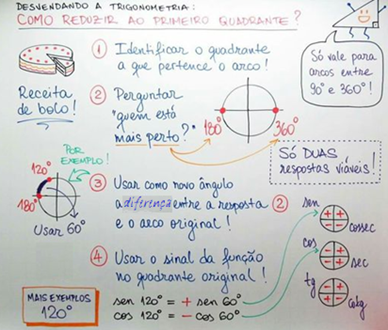
\includegraphics[width=.75\linewidth]{trigonometricas-professor2}
\end{figure}

Cada vez mais tem se desejado um ensino que não tenha foco apenas na memorização de procedimentos e métodos confiáveis para produzir soluções corretas para exercícios resolvidos com papel e lápis e sim que os alunos possam aprender os conceitos de matemática de forma significativa  \citep[Davis, 1993 apud][]{weber2005}. Um ensino focado em regras pode contribuir para que os alunos tenham um conhecimento conceitual inadequado sobre as funções trigonométricas. Há estudos que investigam os principais erros (distratores) que os alunos cometem em trigonometria e muitas vezes eles estão associados a vulnerabilidades conceituais. Por exemplo, um aluno pode ser capaz de calcular o cosseno de um arco do $2$\super{o} quadrante, tendo o valor do seno desse arco. Porém ele não é capaz de explicar qual o significado da expressão “$\sen(x)$”{} para um arco “$x$”{} do $2$\super{o} quadrante.

Em um estudo com alunos de um curso de trigonometria em uma universidade no sul dos Estados Unidos, \cite{weber2005} percebeu que a primeira limitação no entendimento dos alunos sobre funções trigonométricas diz respeito ao papel que as figuras geométricas desempenham na compreensão dessas funções. Ainda de acordo com esse autor, relacionar claramente as funções trigonométricas com modelos geométricos apropriados é importante para entender essas funções.


Destacamos a seguir vulnerabilidades destacadas por alguns autores:

\begin{itemize}
\item Achar que as funções trigonométricas são lineares, escrevendo $\cos(a+b) = \cos(a)+\cos(b)$. \citep{siyepu2015}
\item Dificuldades na compreensão do conceito de radiano. Muitos alunos consideram ângulo em radiano apenas quando π está presente e que, embora consigam fazer corretamente a conversão de ângulos de grau para radiano, eles não conseguem trabalhar bem com ângulos quando apresentados como um número real, sem notação de grau \citep{orhun2010}. Tal fato é corroborado na pesquisa realizada por \cite{feijo2017}, na qual através de questionários e entrevistas o autor percebeu que os alunos não compreendem a definição de radiano, sendo que uma das poucas associações que conseguem fazer é com o número  $\pi$.
\item Confundem medida em radiano com grau, por exemplo: $\sen(29^{\circ}) = \sen(29)$. \citep{orhun2010}
\item Não conseguem ver que as funções trigonométricas são definidas para valores reais, medidos em radianos (acham que o domínio da função seno é $[0,360]$. \citep{orhun2010}
\item Não conseguem estimar o valor do seno de um arco não notável, (ex.: $20^{\circ}$), assim como também encontram dificuldades em indicar qual entre dois arcos têm o maior seno. \citep{weber2005}
\item Dificuldades para reconhecerem ângulos negativos e ângulos maiores que $\frac{\pi}{2}$. \citep{feijo2017}.
\end{itemize}

Em vista de todas essas informações apresentadas até aqui, pretendemos desenvolver neste capítulo um itinerário pedagógico que permita ao professor mediar o desenvolvimento de seus alunos do Ensino Médio na seguinte habilidade da Base Nacional Comum Curricular:


\begin{habilities}{EM13MAT306}
Resolver e elaborar problemas em contextos que envolvem fenômenos periódicos reais (ondas sonoras, fases da lua, movimentos cíclicos, entre outros) e comparar suas representações com as funções seno e cosseno, no plano cartesiano, com ou sem apoio de aplicativos de álgebra e geometria.
\end{habilities}

Nossa abordagem utilizará uma conjugação das metodologias de resolução de problemas, da modelagem matemática aplicada ao seu ensino, além de recursos tecnológicos digitais. Muitos pesquisadores da área de Educação Matemática têm defendido estas metodologias a fim de tornar o processo de aprendizagem da Matemática mais agradável para o aluno, dando-lhe mais protagonismo neste processo. De acordo com \cite{bassanezi1999}, a modelagem matemática “consiste na arte de transformar problemas da realidade em problemas matemáticos, resolvê-los e, então, interpretar suas solucões na linguagem do mundo real, é um processo dinâmico e atraente”. Assim, atividades pedagógicas exploratórias tomando como pontapé inicial a investigação de problemas e a determinação de modelos, que buscam um caminho oposto ao de se iniciar com o conceito já pronto e acabado, frequentemente podem auxiliar o aluno a compreender melhor os argumentos e os conceitos envolvidos de forma mais significativa \citep{bassanezi1999}.  

Com relação aos recursos tecnológicos digitais, \cite{ferreira2013} afirmam que eles permitem realizar simulações, revisões e adaptações, proporcionando um campo pedagógico fértil quer na abordagem de problemas interessantes e instigadores, quer na análise de dados, em argumentações e em tomadas de decisão, de forma que o aluno é conduzido a refletir tanto sobre as informações obtidas quanto sobre as respostas encontradas para os problemas formulados. 

Em nossa abordagem, utilizaremos atividades experimentais que motivem a definição das funções seno e cosseno envolvendo fenômenos periódicos. Na modelagem de alguns desses fenômenos, o aluno poderá perceber que há uma relação entre a sua descrição matemática e as razões trigonométricas estudadas na trigonometria clássica, o que será o pontapé para a construção da generalização de seno e cosseno como funções de $\R$ em $\R$. Algumas das atividades são realizadas com recursos digitais como a plataforma Desmos e o GeoGebra, além o aplicativo Oscilloscope, que permite explorar as ondas sonoras e a sua relação com o comportamento de uma função periódica. No mapa conceitual a seguir ilustra a abordagem de conteúdos que será realizada neste capítulo:

\begin{figure}[H]
\centering

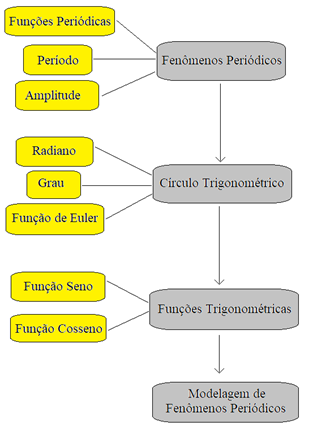
\includegraphics[width=.625\linewidth]{trigonometricas-professor3}
\end{figure}

Não nos aprofundaremos em aspectos mais algébricos de identidades, equações e inequações trigonométricas, buscando consonância com Parâmetros Curriculares Nacionais, os quais mencionam que:

\begin{quote}

(...) a relação da aprendizagem de Matemática com o desenvolvimento de habilidades e competências e a Trigonometria, desde que seu estudo esteja ligado às implicações, \textbf{evitando-se o investimento excessivo no cálculo algébrico das identidades e equações} para enfatizar os aspectos importantes das funções trigonométricas e da análise de seus gráficos. Especialmente para o indivíduo que não prosseguirá seus estudos nas carreiras ditas exatas, o que deve ser assegurado são as aplicações da Trigonometria na resolução de problemas que envolvam medições, em especial o cálculo de distâncias inacessíveis, e \textbf{na construção de modelos que correspondam a fenômenos periódicos}. 

\flushright
\citep[grifo nosso]{PCNEM2000}
\end{quote}


\subsection{Objetivos Gerais}

\begin{enumerate}[label=\titem{\arabic*.}]
\item Identificar um fenômeno periódico e compreender o conceito de função periódica, assim como seu respectivo período;
\item Compreender as definições de círculo trigonométrico, arcos orientados e a relação entre as unidades de medida grau e radiano;
\item Compreender a definição da Função de Euler, assim como os conceitos de seno e cosseno de um número real;
\item Saber esboçar os gráficos de funções seno e cosseno (senóides) e reconhecer os parâmetros que afetam o seu formato, como por exemplo, a frequência e amplitude.
\item Saber utilizar senóides para modelar alguns fenômenos periódicos, assim como realizar previsões com o modelo obtido.
\end{enumerate}




\end{apresentacao}


\def\currentcolor{session1}
\begin{texto}
{
	\paragraph{Objetivo geral da seção}
	\begin{itemize}
	\item Reconhecer o padrão de repetição que ocorre nos pontos do
	gráfico de uma função que modela um fenômeno periódico.
	\end{itemize}


	\paragraph{Sugestões e discussões}
	\begin{itemize}
	\item Nesta primeira seção, vamos explorar alguns exemplos de
	fenômenos periódicos. As atividades aqui descritas visam
	introduzir conceitos de período e de função periódica, assim
	como as características gráficas desse tipo de função.
	Lembramos que as funções trigonométricas são as mais
	adequadas para realizarmos a modelagem de tais fenômenos
	\citep{Lima2006}. Sendo assim, essa primeira seção será
	muito importante para motivar a introdução do conceito de
	seno e cosseno na perspectiva da teoria de funções reais.
	\item As atividades são ordenadas de forma que, ao término de
	cada uma delas, se compreenda com mais detalhes como será
	o formato dos gráficos das funções que modelam esses
	fenômenos. A dedução da expressão analítica que fornece o
	valor exato das imagens dessas funções será realizada nas
	seções posteriores do capítulo.
	\end{itemize}
}
\end{texto}
\begin{objectives}{Pêndulo de um relógio}
{
\begin{itemize}
\item Reconhecer de fenômenos periódicos
\item Construir gráficos de fenômenos que podem ser modelados
por função periódica
\end{itemize}
}{1}{1}
\end{objectives}
\begin{sugestions}{Pêndulo de um relógio}
{
Nesta atividade, espera-se que o aluno consiga perceber o
movimento de “sobe e desce”{} que o gráfico da função que
modela o movimento possui. Além disso, espera-se que ele
perceba que esse movimento se replica à direita quando a
variável do domínio (tempo) aumenta, sendo então diferente
dos gráficos das funções estudadas até aqui. Não há problema
de, nesse momento, o gráfico apresentar imperfeições como
por exemplo, ser construído através de segmentos de reta que
sobem e descem. A atividade seguinte, que tem um cunho
experimental possibilitará ao aluno perceber que o gráfico,
além de ter os comportamentos acima destacados, precisa ter
um formato “arredondado”, se aproximando então da curva
senóide a ser definida nas seções posteriore
}{1}{1}
\end{sugestions}
\clearmargin
\clearmargin
\begin{objectives}{Construindo o próprio pêndulo}
{
\begin{itemize}
\item Apresentar os fenômenos periódicos por uma perspectiva
empírica
\item Construir gráfico de fenômeno que pode ser modelado por
função periódica
\end{itemize}
}{1}{1}
\end{objectives}
\begin{sugestions}{Construindo o próprio pêndulo}
{
Ao término dessa atividade, é importante comparar
os gráficos obtidos com aqueles construídos na atividade
anterior. Como o movimento a ser modelado nas duas
atividades é essencialmente o mesmo, o gráfico construído
nesta segunda atividade, de forma experimental e com mais
precisão contribuirá para que o aluno reflita sobre possíveis
imperfeições existentes no formato dos gráficos obtidos na
atividade anterior.

Uma outra maneira de se construir um pêndulo simples, mas
com borracha, tubo de caneta, linha de costura e fita adesiva
pode ser visto na atividade 5 de: \url{http://www.aprendizagemconectada.mt.gov.br/documents/14
069491/14094177/Semana+04-08+de+maio/cb1df5e3-7082-
b9a1-be1f-714c5f25265d}
}{1}{1}
\end{sugestions}
\clearmargin
\vspace{.5em}
\begin{answer}{Construindo o próprio pêndulo}
{
\begin{enumerate}
\item ---
\item Movimento de “sobe e desce”{} e de repetição do mesmo
com o passar do tempo (movimento periódico)
\item São similares, com repetição de um padrão, mas neste
último gráfico, o formato arredondado ficará mais evidente,
fazendo com que o aluno reflita sobre possíveis imperfeições
nos desenhos da atividade anterior
\end{enumerate}
}{1}
\end{answer}
\begin{objectives}{Construindo uma Roda Gigante}
{
\begin{itemize}
\item Apresentar fenômenos periódicos por uma perspectiva
empírica
\item Construir gráfico de fenômeno que pode ser modelado por
função periódica
\item Identificar alguns elementos das funções periódicas
\end{itemize}
}{1}{2}
\end{objectives}
\begin{sugestions}{Construindo uma Roda Gigante}
{
Nesta atividade, além de apresentar um novo exemplo de
fenômeno periódico, pretende-se começar a explorar e
aprimorar conceitos associados a funções periódicas como
período e seus reflexos no gráfico da função (itens \titem{b)}, \titem{g)} e \titem{h)}), conjunto imagem, valor máximo e mínimo (itens \titem{d)} e
\titem{e)}) e o próprio formato não-retilíneo do gráfico da função
que modela esse exemplo (item \titem{f)}).
}{1}{2}
\end{sugestions}
\clearmargin
\marginpar{\vspace{.5em}}
\begin{answer}{Construindo uma Roda Gigante}
{
\begin{enumerate}
\item Isso irá depender da roda gigante construída para o
experimento.
\item $18$ segundos.
\item atividade prática.
\item Sim, todas as alturas intermediárias são atingidas 2 vezes
\item Isso dependerá da altura da roda gigante construída.
\item Não. Os instantes em que a cabine passa por pontos onde a
reta tangente à circunferência da roda gigante terão variação
da altura maior do que quando a cabine está no topo da roda
por exemplo.
\item Para $t>18$, o gráfico é a repetição
\item A função oscilaria mais rápido O gráfico ficaria mais
“comprimido”.
\end{enumerate}
}{1}
\end{answer}
\clearmargin
\begin{answer}{Para Refletir: Roda Gigante Virtual}
{
Resposta à $1$\super{a} pergunta: O gráfico seria uma translação horizontal do gráfico obtido na atividade anterior, de forma que um de seus pontos mais altos intersectaria o eixo $y$.

Resposta à $2$\super{a} pergunta: O gráfico faria seu movimento oscilatório de sobe e desce de forma mais devagar. Assim, o gráfico ficaria mais “alongado”
}{1}
\end{answer}
\explore{Fenômenos Periódicos}
\label{trig-exp1}

Iniciaremos este capítulo estudando exemplos de fenômenos do nosso cotidiano que têm uma propriedade até então não observada nos capítulos anteriores do livro de Funções: são fenômenos que se repetem com o passar do tempo. Um dos objetivos desse capítulo é estudar técnicas de modelagem matemática desse tipo de fenômeno, visando antever situações relacionadas a ele. Quais seriam as funções adequadas para realizar essa modelagem? Realizando as atividades a seguir, você irá aos poucos descobrir que funções são essas e que características algébricas e gráficas elas possuem.

\begin{task}{Pêndulo de um relógio}
\textit{(Adaptado de \cite{costa2017})}
\label{trig-ativ1}

Alguns relógios rústicos têm um pêndulo, composto por uma bolinha presa à parte de baixo de uma haste que oscila continuamente de um lado para o outro. O fato de o pêndulo estar em movimento mostra que o relógio está em pleno funcionamento.

\begin{figure}[H]
\centering

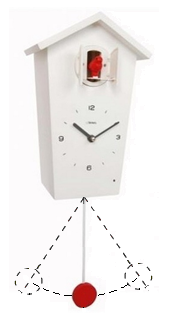
\includegraphics[width=.25\linewidth]{trigonometricas1}
\end{figure}

Vamos estudar o comportamento da projeção do centro dessa bola numa reta horizontal localizada abaixo desse relógio, supondo que a origem dessa reta coincida com a projeção do centro da bola quando a haste do pêndulo está na posição vertical. Em outras palavras, vamos estudar as variações dos pontos da reta alcançados pela projeção do centro da bola. As imagens a seguir ilustram algumas possíveis posições do pêndulo. O centro do pêndulo está representado pelo ponto $E$; os pontos $C$ e $B$ são os pontos extremos do caminho percorrido pelo pêndulo. O ponto $O$ é aquele em que o pêndulo se encontra preso ao relógio. O ponto $F$ indica possíveis posições do pêndulo, e o ponto $G$ indica a projeção de $E$ na reta orientada a seguir. Observe as diferentes posições de $F$ ilustradas e os valores da distância entre $A$ e $G$ ($A$ é a projeção de $O$ na reta orientada). A construção no GeoGebra do movimento de um pêndulo similar a esse pode ser acessada no link \url{https://www.geogebra.org/classic/uxcqamaz}


\begin{figure}[H]
\centering

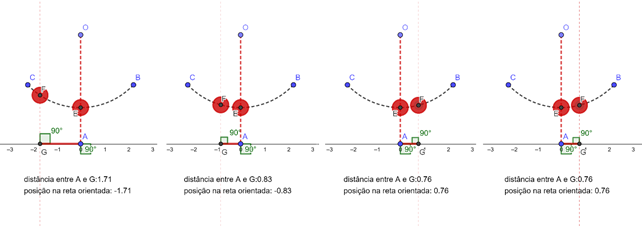
\includegraphics[width=\linewidth]{trigonometricas2}
\end{figure}

Suponha que no tempo $t$, a função que descreve o deslocamento dessa projeção seja $d(t)$. Note que, como estabelecemos uma posição como origem, esta função é considerada com sinal assumindo um valor positivo quando o pêndulo estiver à direita do segmento $OA(d(t_1)\geq0)e$ assumindo um valor negativo quando estiver à esquerda de $OA(d(t_2)\leq0)$, conforme é possível ver na ilustração acima: a distância entre $A$ e $G$ é um módulo, é absoluta; no entanto, quando consideramos a posição na reta orientada, atribuímos um sinal a essa distância.

\begin{figure}[H]
\centering

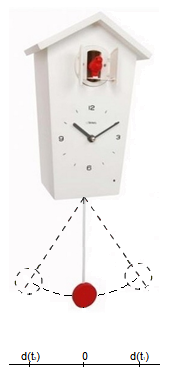
\includegraphics[width=.25\linewidth]{trigonometricas3}
\end{figure}

\begin{enumerate}
\item Na malha quadriculada abaixo, considere $D_{\max}$ e $E_{\max}$ o maior e o menor valor assumidos pela função $d$. Repare que $D_{\max}$ corresponde à projeção do ponto $B$ na reta horizontal, que é o ponto mais à direita que é atingido pelo centro da bolinha ao longo da oscilação do pêndulo. Da mesma forma, $E_{\max}$ corresponde à projeção de $C$, que é o ponto mais à esquerda que é atingido pelo centro da bolinha durante o movimento. Tente esboçar o gráfico da função $d(t)$, supondo que $d(0) = D_{\max}$.

\begin{figure}[H]
\centering

\resizebox{.75\linewidth}{!}
{
\begin{tikzpicture}
\draw [step=.5,gray!50] (-1.5,-7) grid (14,7);
\draw [->] (-1.5,0) -- (14,0) node [below left, thick] {Tempo};
\draw [->] (0,-7) -- (0,7) node [below right, thick] {Distância da massa ao centro};
\draw (.1,3) -- (-.1,3) node [left, overlay] {$D_{\max}$};
\draw (.1,-3) -- (-.1,-3) node [left, overlay] {$E_{\max}$};
\end{tikzpicture}
}
\end{figure}

\item Que aspectos você percebe que esse gráfico possui? Cite algumas diferenças entre ele e os gráficos das funções que você estudou até aqui.
\end{enumerate}
\end{task}

\begin{task}{Construindo o próprio pêndulo}
\textit{(Adaptado de \cite{costa2017})}
\label{trig-ativ2}

Com madeira, um prego, barbante e uma bolinha de gude, construir um pêndulo como o da figura. 

\begin{figure}[H]
\centering

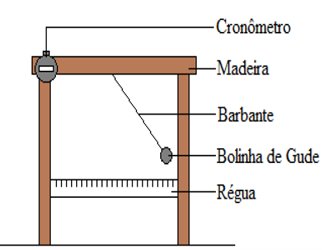
\includegraphics[height=.225\textheight]{trigonometricas5}
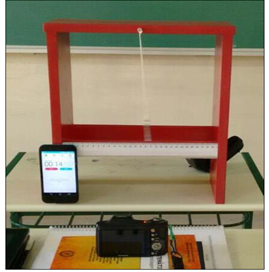
\includegraphics[height=.225\textheight]{trigonometricas6}

\caption{\cite{costa2017}}
\end{figure}

Será necessário o uso de dois celulares ou um celular e uma câmera. Um dos celulares irá cronometrar o tempo durante a oscilação do pêndulo e o outro, deverá tirar sucessivas fotografias do movimento do pêndulo e do primeiro celular. Uma régua deve ser utilizada também para medir o deslocamento horizontal da projeção do pêndulo, como na figura acima. Posicione o pêndulo exatamente sobre o zero da régua e solte-o no momento em que cronômetro for ligado e as fotos começarem a ser tiradas. Fotografar o movimento ao longo de 4 oscilações completas do pêndulo.

\begin{enumerate}
\item Analise as fotografias e forme pares ordenados $(x,y)$ onde $x$ representa o tempo e $y$, a medida na régua na qual estará a projeção horizontal do pêndulo.

\item Plote os pontos no GeoGebra. Que comportamento você consegue perceber no caminho que os pontos vão percorrendo?
\item Compare o esboço que você obteve aqui com o da atividade anterior. Que conclusões você consegue tirar?
\end{enumerate}


\end{task}


\begin{task}{Construindo uma Roda Gigante}
\label{trig-ativ3}

Utilizando papelão, tampinhas de garrafa, cola e um lápis, construir uma roda gigante como a da figura.

\begin{figure}[H]
\centering

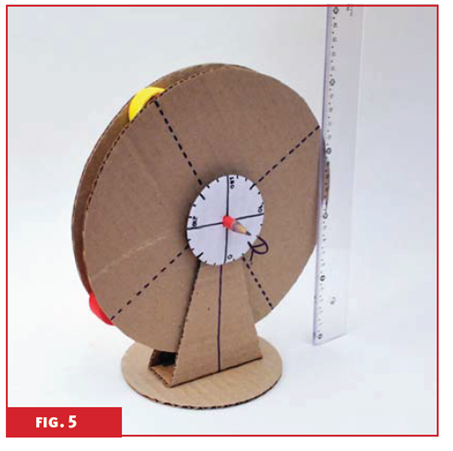
\includegraphics[width=.45\linewidth]{trigonometricas7}
\caption{Fonte: \cite{soares2010}}
\label{}
\end{figure}

Será necessário também o uso de um transferidor para medir os ângulos e uma régua para medir a altura das “cabines”.

Um passageiro entra na cabine quando essa está em seu ponto mais baixo. A partir daí, a roda começa a girar no sentido anti-horário, numa velocidade constante de $20$ graus por segundo. Considere $h = h(t)$ a altura em centímetros da cabine no instante de tempo $t$, medido em segundos.
\begin{enumerate}
\item Calcule a medida do raio da roda gigante e também as alturas mínima e máxima que a cabine pode assumir.
\item Quantos segundos a roda gigante demora para dar uma volta completa?
\item Com o auxílio dos seus colegas, encontre a altura da cabine em cada segundo do movimento da roda gigante até ela completar uma volta. Marque num papel milimetrado os pontos $(t,h(t))$ obtidos.
\item Entre a altura máxima e a altura mínima, há alguma altura intermediária que a cabine atinge mais de uma vez ao longo de cada volta da roda gigante? Quanto mede essa altura intermediária?
\item Determine todos os valores assumidos pela altura h da cabine ao longo de uma volta completa da roda gigante.
\item Observando os pontos marcados no item \titem{c)} e a dinâmica do giro da roda gigante, responda: apesar da velocidade com que a roda gigante gira ser constante, também será constante a taxa de variação da altura da cabine?  
\item Esboce no papel milimetrado uma curva que represente o gráfico de função $h = h(t)$. Como será o gráfico da função para valores de $t$ maiores que $18$ s?
\item Como seria o gráfico de $h = h(t)$ se a velocidade do giro da roda gigante duplicasse, ou seja, se ela demorasse apenas $9$ s para dar uma volta completa? Que alterações podem ser observadas em relação ao gráfico traçado no item \titem{g)}?
\end{enumerate}

\end{task}


\begin{reflection}
\label{trig-reflection1}
\vspace{-2\parskip}
\paragraph{Roda Gigante Virutal}

Acesse o link de uma roda gigante construída virtualmente no GeoGebra através do seguinte link \url{https://www.geogebra.org/m/g8mnxpgx}

Também é possível visualizar nesse link o gráfico que relaciona a altura da cabine da roda gigante virtual com o tempo.

\begin{figure}[H]
\centering

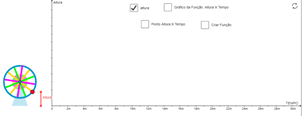
\includegraphics[height=.11\textheight]{trigonometricas8}
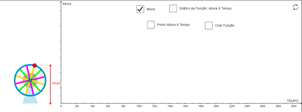
\includegraphics[height=.11\textheight]{trigonometricas9}
\caption{Observação da altura da cabine}

\end{figure}

\begin{figure}[H]
\centering

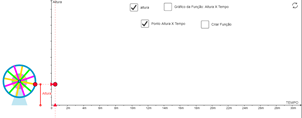
\includegraphics[height=.11\textheight]{trigonometricas10}
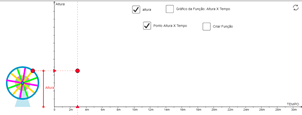
\includegraphics[height=.11\textheight]{trigonometricas11}
\caption{Observação do ponto do plano que associa a $x$ o tempo e a $y$ a altura da cadeira}
\end{figure}

\begin{figure}[H]
\centering

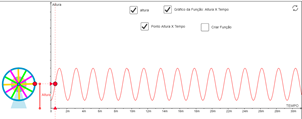
\includegraphics[height=.11\textheight]{trigonometricas12}
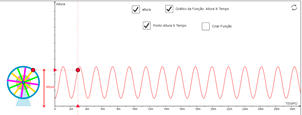
\includegraphics[height=.11\textheight]{trigonometricas13}
\caption{Observação do gráfico da função que associa a $x$ o tempo e a $y$ a altura da cadeira}
\end{figure}

Compare esse gráfico com o gráfico obtido por você e seus colegas na atividade anterior. Como você acha que deveria ser o gráfico se o movimento começasse quando a cabine estivesse no ponto mais alto da roda? E como seria o gráfico se a velocidade com que a roda gigante gira fosse reduzida à metade?
\end{reflection}

\clearpage
\begin{texto}
{	\def\currentcolor{session4}
	\paragraph{Objetivo geral da seção}
	\begin{itemize}
	\item Formalizar os conceitos e elementos dos fenômenos e das
	funções periódicas
	\end{itemize}

	\paragraph{Sugestões e discussões}

	Para organizar os conceitos de fenômenos e
	funções periódicas, assim como seus elementos,
	exploraremos bastante a atividade construindo uma roda
	gigante

}
\end{texto}
\arrange{Fenômenos Periódicos.}
\label{trig-arg1}

O que os fenômenos apresentados nas atividades anteriores têm em comum? Se considerarmos uma situação ideal em que o mesmo fenômeno se repete \textit{exatamente} da mesma maneira ao longo do tempo, podemos dizer que o pêndulo do relógio sempre vai e volta ininterruptamente e que a roda gigante dá várias voltas sem parar. Fenômenos assim são chamados de \textit{periódicos}, ou seja, que se repetem exatamente da mesma forma ao longo do tempo. Ao estudarmos matematicamente as situações que usamos como exemplo aqui, consideramos um modelo. Um \textit{modelo matemático} é uma descrição matemática a partir da observação de algum fenômeno observado no mundo físico. Claro que, ao fazermos essa descrição em termos matemáticos, precisamos fazer algumas restrições e suposições que não necessariamente ocorreram ou ocorreriam de fato no fenômeno observado - mas, com um modelo, é razoável que consideremos essas restrições. Por exemplo, a suposição de que um pêndulo como o da primeira ou da segunda atividade oscila ininterruptamente não ocorre no mundo real: o relógio pode atrasar por algum problema no mecanismo ou até mesmo parar, por exemplo. A roda gigante precisa parar sempre que alguém vai subir ou descer do brinquedo. Mas, as restrições que são feitas para criar o modelo possibilitam que o fenômeno seja estudado, que previsões sejam feitas, além de permitir que outros fenômenos sejam classificados por semelhanças ou diferenças.

Você conhece mais alguns fenômenos periódicos que acontecem na vida?


\begin{figure}[H]
\centering

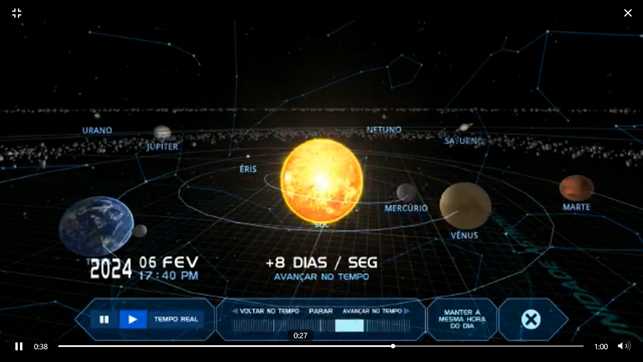
\includegraphics[width=.75\linewidth]{trigonometricas14}
\caption{Fonte: \href{https://www.solarsystemscope.com/}{Solar System Scope}}
\label{}
\end{figure}

O movimento de rotação da Terra em torno de seu próprio eixo é um movimento periódico que demora $24$ h para completar um ciclo (período de $24$ h) e o movimento de translação da Terra ao redor do Sol demora $365$ dias e $6$ h para completar um ciclo (período de $365$ dias e $6$ h).

Nas atividades anteriores você fez os gráficos de funções que representam fenômenos periódicos. Por esse motivo elas também serão chamadas de \textit{funções periódicas}, ou seja, funções cujos valores da imagem se repetem em intervalos fixos. Mais precisamente, uma função $y=f(x)$ é chamada de periódica, se existe algum valor $p$ tal que $f(x)=f(x+p)$, para todos os valores de $x$ tais que $x$ e $x+p$ pertençam ao domínio dessa função. O menor valor positivo de $p$ que satisfizer a essa propriedade será chamado o período dessa função.

Para entender melhor os conceitos que estamos apresentando, vamos discutir um pouco sobre a Atividade \hyperref[trig-ativ1]{“Construindo uma Roda Gigante”}. Nela, você foi orientado a observar o comportamento de uma cabine em específico. Como a roda gigante tem velocidade de rotação constante, o comportamento se repete a cada volta. Isso significa que o gráfico que você gerou para a primeira volta completa da roda gigante vai se repetir exatamente dessa mesma forma por todo o tempo em que a roda gigante permanecer girando. Esse é, portanto, um \textit{fenômeno periódico}.


A velocidade de rotação é de $20$ graus por segundo; logo, uma volta completa ($360^{\circ}$) será alcançada após $18$ segundos. Decorridos os primeiros $18$ segundos de movimento, a roda gigante vai ter dado uma volta completa e a cabine observada terá voltado para sua posição inicial. Matematicamente, podemos escrever que $h(0)=h(18)$. Independentemente da posição ocupada pela cabine no instante $t$, após $18$ segundos a roda gigante dará uma volta completa e a cabine voltará para a mesma posição em que estava quando começamos a marcar o tempo. Matematicamente, essa observação pode ser registrada como  $h(t)=h(t+18)$. É interessante observar que isso é verdade para outros valores: por exemplo, após 36 segundos, a roda gigante terá dado $2$ voltas, portanto $h(t)=h(t+36)$.
De maneira mais geral, considerando um número inteiro positivo k, a roda gigante terá dado $k$ voltas após $18k$ segundos  e, portanto, $h(t)=h(t+18k$), o que indica que essa função é periódica de período $18$, pois esse é o menor valor necessário para que se tenha um ciclo completo do fenômeno observado, ou seja, da roda gigante em movimento.

Mas será que esse é de fato o menor valor para o qual esse ciclo se repete? Note que, por exemplo, quando $t=4{,}5$, a roda gigante terá dado $\frac{1}{4}$	de volta, e portanto, $h(4{,}5)=r$. Após $9$ segundos, a roda gigante terá dado mais $\frac{1}{2}$ volta, assim, a cabine estará a mesma altura que estava no instante $t=4{,}5$, o que indica que $h(4{,}5)=h(4{,}5+9)$. Será que isso significa que $9$ pode ser o período dessa função? Se isso fosse verdade, precisaríamos ter $h(t)=h(t+9)$, para todos os valores $t$ do domínio; no entanto, isso não é verdade, uma vez que no instante $t=0$ a cabine está na posição mais baixa e no instante $t=9$, a roda gigante terá dado $\frac{1}{2}$ de volta e, portanto, a cabine estará na posição mais alta e não de volta ao início, como seria necessário. Note ainda que depois do instante $t=0$, a cabine só voltará para a posição inicial após dar uma volta completa, portanto, após $18$ segundos. Logo, não existe p$<18$ tal que $h(0)=h(0+p)$; ou seja, o período é, de fato $18$.

Repare que, uma vez conhecido o comportamento do gráfico dessa função na faixa $0\leq t\leq18$, também conhecemos o comportamento dela na faixa $18\leq t\leq 36$: será exatamente a repetição do gráfico da faixa anterior, uma vez que a partir de $t=18$ a função se comporta da mesma maneira que se comportava entre $t=0$ e $t=18$. De maneira mais geral, o gráfico na faixa $18k\leq t\leq 18(k+1)$ será uma cópia da faixa do gráfico na faixa $0\leq t\leq 18$.

O período desempenha um papel importante no gráfico de uma função periódica: se conhecermos o desenho do seu gráfico num trecho sobre um intervalo do domínio de comprimento p então podemos esboçar o gráfico inteiro da função, “copiando e colando”{} esse trecho ao longo de todo o domínio.

\begin{figure}[H]
\centering

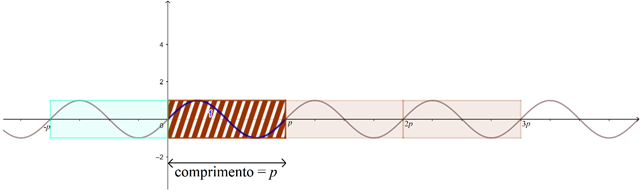
\includegraphics[width=.9\linewidth]{trigonometricas15}
\end{figure}

A amplitude é outra característica importante quando estudamos uma função periódica. Quando a imagens $f(x)$ de uma função periódica assumirem um valor máximo $M$ e também um valor mínimo m, definimos a \textit{amplitude} de $f$ como sendo $a=\frac{(M-m)}{2}$. Geometricamente, a menor faixa horizontal que contém o gráfico da função $f$ terá largura igual ao dobro da amplitude.

\begin{figure}[H]
\centering

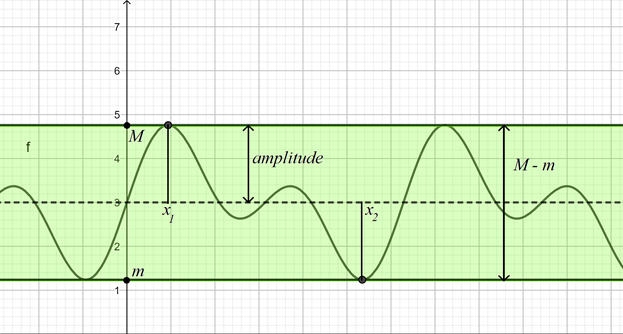
\includegraphics[width=.7\linewidth]{trigonometricas16}
\end{figure}

Na figura a seguir, vemos o gráfico de uma função f definida no intervalo $[-5,5]$, conhecida na literatura como \textit{função dente de serra}.

\begin{figure}[H]
\centering

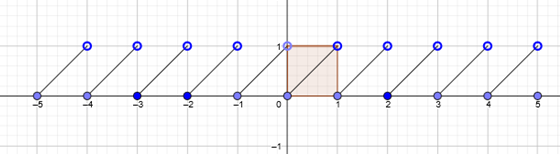
\includegraphics[width=.75\linewidth]{trigonometricas17}
\end{figure}


Podemos perceber que este gráfico é formado por um conjunto de segmentos de reta que são paralelos, sendo que um desses segmentos tem extremidades nos pontos $(0,0)$ e $(1,1)$ e os outros são réplicas desse mesmo trecho do gráfico que se repetem para a esquerda e para a direita. Repare que o ponto $(1,1)$ do segmento replicado é omitido, senão a figura resultante não representaria o gráfico de uma função (Por quê?).

Repare que, para qualquer número $0 < p < 1$, o trecho do gráfico que fica sobre o intervalo $[0, p]$ no eixo $x$ corresponde apenas a uma parte de um desses segmentos de reta, de forma que ao replicarmos essa parte para a esquerda e para a direita, obteríamos uma figura diferente do gráfico da função. Portanto, nenhum número menor que $1 $pode ser o período de $f$. Concluímos que $p =1$ é o \textbf{período} da função.

Como o menor valor e o maior valor assumidos pela imagem são $0$ e $1$ respectivamente, temos que a amplitude é igual $\dfrac{(1-0)}{2}=\dfrac{1}{2}$.

Isso nos mostra que podemos criar uma infinidade de funções periódicas agindo exatamente dessa mesma forma! Podemos definir uma função em um determinado intervalo, por exemplo, $[-2, 0]$, e a partir daí reproduzir por intervalos sucessivos translações horizontais que tenham como fator de translação o mesmo comprimento do intervalo usado como base para criar a função.

\practice{Fenômenos periódicos}
\label{trig-prac1}
\phantom{M}
\vspace{-1em}
\vspace{-\baselineskip}

\begin{answer}{Rio Star}
{
	\begin{enumerate}
	\item $42{,}5$ mts
	\item Não, pois o ponto mais baixo da roda gigante está a $3$ mts
	do chão
	\item Mesma altura do centro: $4$ min e $30$ seg, $13$ min e $30$ seg,
	$22$ min e $30$ seg e $31$ min e $30$ seg.

	Pontos mais altos: $9$ e $27$ min

	Pontos mais baixos: $0$, $18$ e $36$ min
	\item Não. No intervalo $[0; 4{,}5]$ do tempo, a cadeira parte da
	posição mais baixa na roda gigante e gira um quarto de volta,
	atingindo a altura do centro da roda. Nos dois minutos
	iniciais, a cadeira se encontra no ponto mais baixo da roda e
	quando esta começa a girar, o deslocamento horizontal da
	cabine inicialmente será maior que o vertical. Nos dois
	minutos seguintes, a situação se inverte, aumentando mais o
	deslocamento vertical da cadeira em relação ao horizontal.
	Portanto, nos primeiros dois minutos de movimento a cadeira
	subirá uma altura menor que nos dois minutos seguintes.
	\item Período: $18$; Imagem: $[3;88]$; amplitude: $42{,}5$
	\end{enumerate}
}{1}
\end{answer}
\clearmargin
\begin{sugestions}{Construa sua própria função periódica!}
{
	Caro professor, essa atividade é totalmente pessoal. É muito importante iniciar com o aluno determinando os eixos coordenados onde estarão para que assim ele possa situar a sua curva de maneira a correlacioná-la com alguma situação real e determinar período e amplitude. Uma ideia poderia ser o consumo de água de uma residência com 4 pessoas, suposto regular, durante o período de um dia em tempos de pandemia, em que os moradores não se ausentam de casa e realizam ali todas as refeições - tempo total: $20$ dias de observação, registros de consumo verificados a cada $6$ h, a partir das 6hrs da manhã, pensados em intervalos de madrugada ($0$ h-$6$ h), manhã ($6$ h-$12$ h), tarde ($12$ h-$18$ h), noite ($18$ h-$0$ h). Os registros diários de consumo seriam, por exemplo:
	\begin{itemize}[topsep=2pt]
	 \item madrugada - $20\ell$; 
	 \item manhã - $500\ell$; 
	 \item tarde - $60\ell$; 
	 \item noite - $300\ell$;
	 \end{itemize}
	 O gráfico poderia ser composto por uma linha poligonal, começando num ponto de ordenada $50$, depois passando por outro com ordenada $500$, depois por outro de ordenada $60$, outro de ordenada $300$ e em seguida um de ordenada $20$ e finalizando com outro ponto de ordenada $50$ (encerrando assim um ciclo do período da função). O gráfico da função periódica seria a repetição dessa poligonal. Teríamos então o gráfico sugerido a seguir, no qual o período é de $24$ h e a amplitude é $\frac{|20 - 500|}{2}=240$. Uma ideia interesse seria fazer uma análise crítica do contexto pensado com o gráfico produzido e pensar que modificações poderiam ser feitas no gráfico para que ele se adaptasse melhor ao contexto, numa perspectiva similar à realizada nas atividades do pêndulo realizadas no início do capítulo.
}{1}{1}
\end{sugestions}
\clearmargin
\clearmargin
\clearmargin
\marginpar{\vspace{.5em}}
\begin{answer}{Bem estar digital}
{
\begin{enumerate}[left=7.5pt, wide]
\item \adjustbox{valign=t}
{
\scalebox{.9}
{
\begin{tabular}{|e{.3\linewidth}|e{.3\linewidth}|e{.3\linewidth}|}
\hline
\tcolor{Dia da Semana} & \tcolor{N\super{o} de mensagens recebidas} & \tcolor{N\super{o} de vezes que o aplicativo foi aberto} \tabularnewline
\hline
1 (qui) & $764$ & $150$ \tabularnewline
\hline
2 (sex) & $641$ & $130$ \tabularnewline
\hline
3 (sáb) & $762$ & $176$ \tabularnewline
\hline
4 (dom) & $20$ & $7$ \tabularnewline
\hline
5 (seg) & $416$ & $96$ \tabularnewline
\hline
6 (ter) & $1913$ & $148$ \tabularnewline
\hline
7 (qua) & $872$ & $164$ \tabularnewline
\hline
\end{tabular}
}
}
\item [\titem{b)} e \titem{c)}] Esses gráficos foram construídos no GeoGebra para Smartphone, a versão Suite GeoGebra
Calculadora, que mescla funções da geometria, da álgebra e planilhas. A função usada foi datafunction({lista de abscissas},{lista de ordenadas}), que associa pontos de um determinado conjunto de dados (se quiser, utilize a opção “Ampliar para enquadrar”{} na Janela de Visualização para conseguir ver a figura como um todo. 

Para o gráfico do número de mensagens por dia da semana, o comando foi 
\begin{center}
\textit{datafunction}($\{1, 2, 3, 4, 5, 6, 7\}, \{764, 641, 762, 20, 416,1913, 872\}$). 
\end{center}
Para o  gráfico do número médio de mensagens por dia da semana, o comando usado foi 
\begin{center}
\textit{datafunction}($\{1, 2, 3, 4, 5, 6, 7\}, \{150, 130, 176, 7, 96, 148, 164\}$).
\end{center}
 Os pontos indicados a seguir foram construídos separadamente, com o objetivo de destacar as informações encontradas na tabela - a saber:
\begin{multicols}{2}
\begin{figure}[H]
\centering
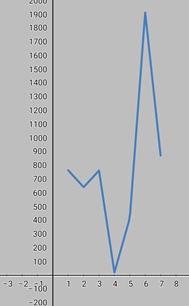
\includegraphics[height=.25\textheight]{trigonometricas29}

\caption{Número de mensagens
recebidas por dia da semana}
\label{}
\end{figure}
\begin{figure}[H]
\centering
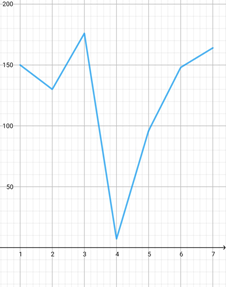
\includegraphics[height=.25\textheight]{trigonometricas30}
\caption{Número de vezes que o
aplicativo foi aberto por dia da semana}
\label{}
\end{figure}
\end{multicols}
\end{enumerate}
}{1}
\end{answer}
\clearmargin
\marginpar{\vspace{.5em}}
\begin{answer}{Bem estar digital}
{
	\begin{enumerate}[left=7.5pt, wide]\setcounter{enumi}{3}
	\item Há uma queda expressiva nas observações ligadas ao dia 4, que é domingo, o que é natural - tanto em relação ao número de mensagens  ecebidas quanto em relação ao número de vezes que o aplicativo foi aberto. De quarta a sábado observa-se uma queda no número de mensagens recebidas, mas há uma maior ocorrência de abertura do aplicativo. Vale a pena incentivar os alunos a buscar esses dados nos seus próprios smartphones, caso exista essa opção nas configurações, e comparar com as rotinas deles, conforme sugerimos no item \titem{f)}

	\item As funções cujos gráficos foram esboçados nos itens b e c não são periódicas, visto a inexistência de um fenômeno cíclico. No entanto, há regularidades que podem ser inferidas a partir da observação das figuras do enunciado, como horários de trabalho - observe que o tempo em que o aplicativo não é aberto é aproximadamente regular ao longo das observações, indicando horário em que a pessoa observada provavelmente está dormindo. Há em geral uma quantidade maior de notificações de mensagens entre os períodos da manhã e tarde, ocorrendo no entanto dias em que isso não se verifica.
	\item Podemos construir gráficos que indiquem a reprodução desses trechos ao longo de novas semanas. Dessa forma, o período dessas funções construídas, desses modelos, seria igual a $7$, visto que o trecho encontrado no intervalo de $1$ a $8$ encontra-se “copiado”. Para ilustrar isso,  podemos usar a transformação translação no GeoGebra, ou simplesmente prosseguir marcando os pontos com as mesmas ordenadas e somando $7$ unidades às abscissas, o que gerará uma translação em $7$ unidades para a direita nos dois gráficos. Para usar o GeoGebra, considerando que já temos os gráficos anteriores prontos na tela, podemos construir os pontos $(1,0)$ e $(8,0)$ e construir o vetor com origem em $(1,0)$ e extremidade em $(8,0)$. O vetor está disponível na galeria de comandos “Retas”:

	\notas{
	\adjustbox{valign=t}
	{
	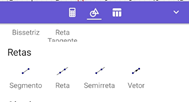
\includegraphics[width=.6\linewidth]{trigonometricas31}
	}
	}

	e então usar a transformação geométrica translação, disponível no menu TRANSFORMAR em Geometria

	\notas{	
	\adjustbox{valign=t}
	{
	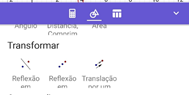
\includegraphics[width=.6\linewidth]{trigonometricas32}
	}
	}

	Ao tocar em translação, precisamos indicar que objeto desejamos transladar e por que vetor. Toque, sequencialmente, após tocar em translação, no gráfico da função e no vetor. Realizando essa mesma sequência novamente de toques a partir sempre da última translação gerada, btemos um gráfico que remete à ideia de uma função periódica. Para a função que representa o número de mensagens recebidas por dia da semana, a amplitude é $\frac{1913−20}{2}= 946{,}5$ e para a função que representa o número de vezes que esse aplicativo foi aberto a cada dia da semana, a amplitude é $\frac{176−7}{2} = 84{,}5$. Para ambas, o período é $8 - 1 = 7$.

	Os dois últimos itens são pessoais. Incentive seus alunos a que busquem conhecer melhor sobre essa ferramenta: essa é uma questão de saúde.
	\end{enumerate}
}{1}
\end{answer}

\begin{sugestions}{Você sabia? -- O Som e as Ondas Sonoras}
{Nesta atividade, pretende-se apresentar ao aluno uma aplicação da noção de função periódica, ilustrando como esse conceito está associado ao som que ouvimos. O aplicativo Oscilloscope é totalmente gratuito e pode ser baixado nos celulares dos alunos. Sons simples produzidos com a própria voz, como “dó”, “ré”, “mi”, falados de forma prolongada, podem reproduzir ondas com formato periódico. É interessante perguntar a eles o que acontece com a onda quando se emite um som cada vez mais alto (e espera-se que eles visualizem que a amplitude da onda está associada à intensidade do som). Da mesma forma, pergunte aos alunos quais as diferenças de formato das ondas quando o som emitido é mais grave ou mais agudo (o período será menor nos sons mais agudos e maior nos mais graves)}
{1}{2}
\end{sugestions}
\clearmargin
\clearmargin
\begin{objectives}{Você sabia? -- Eletrocardiograma}
{
O objetivo deste item é ilustrar mais um exemplo de aplicação das funções periódicas.
}{1}{2}
\end{objectives}
\begin{task}{Rio Star}
\label{trig-ativ4}

\begin{figure}[H]
\centering

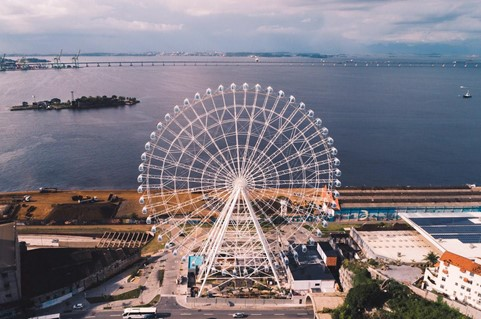
\includegraphics[width=.55\linewidth]{trigonometricas18}
\end{figure}

A Rio Star é a maior roda gigante da América Latina e está localizada na cidade do Rio de Janeiro. Ela tem $88$ metros de altura. A atração turística conta com $54$ cabines climatizadas que podem receber até 8 pessoas cada, totalizando $432$ visitantes que poderão apreciar a vista da Zona Portuária, do Relógio Central, Morro da Providência, Cristo Redentor, Pão de Açúcar, Pedra do Sal, Ponte Rio-Niterói e da Cidade do Samba durante 18 minutos - tempo necessário para a volta completa no brinquedo. (Fonte: \href{https://casavogue.globo.com/LazerCultura/Viagem/noticia/2019/12/rio-star-roda-gigante-do-rio-de-janeiro-inaugura-hoje.html}{Casa Vogue})

Suponha que o ponto mais baixo da roda gigante que qualquer uma das cabines pode atingir se encontra a $3$ metros de altura do chão. Beatriz e Gabriela embarcam em uma das cabines e a partir daí, a roda gigante gira continuamente com a mesma velocidade e dá duas voltas sem parar, finalizando o movimento com a cabine das meninas retornando ao ponto mais baixo.

\begin{enumerate}
\item Qual é o raio da roda gigante?
\item Existe algum momento em que a altura da cabine em relação ao chão será nula? Justifique.
\item Em quais instantes do movimento a cabine estará na mesma altura do centro da roda gigante? E no ponto mais alto da roda? E no ponto mais baixo?
\item Você acha que a altura a que a cabine sobe nos primeiros dois minutos do movimento é a mesma que nos dois minutos seguintes? Justifique sua resposta?
\item No plano cartesiano, plote no plano cartesiano os pontos $(t,h)$ com os dados obtidos no item \titem{c)}, em que $t$ é o tempo e $h$ é a altura da cabine. Em seguida, esboce a curva por meio desses pontos que você acha que representa o gráfico da função altura $h = h(t)$. Compare seu gráfico com o de seus colegas.
\item Qual o período, a amplitude e o conjunto imagem da função $h = h(t)$?
\end{enumerate}
\end{task}

\begin{task}{Construa sua própria função periódica!}
\label{trig-ativ5}

Vamos fazer a nossa própria função periódica?

\begin{enumerate}
\item Usando a malha quadriculada proposta a seguir, defina, a origem, os eixos $Ox$ e $Oy$ e desenhe, usando até $6$ unidades horizontais da malha, uma curva que possa representar o gráfico de uma função, de modo que o ponto inicial da curva tenha mesma altura que o ponto final.
\item Agora, reproduza exatamente esse mesmo trecho por toda a largura da malha, do mesmo jeito como foi feito com a função dente de serra, construindo assim o gráfico de uma função periódica.
\item Qual o período e a amplitude da sua função periódica?
\item Compare o seu gráfico com o de seus colegas. Será que em pelo menos algum deles, você consegue imaginar um contexto real (climática, biológica, doméstica, tecnológica ou outras quaisquer) que ele poderia representar?

\end{enumerate}


\begin{figure}[H]
\centering


\begin{tikzpicture}
\draw [step=.5,gray!50] (-1.5,-5) grid (14,5);
\end{tikzpicture}

\end{figure}
\end{task}

\clearpage
\begin{task}{Bem estar digital}
\label{trig-ativ6}


Veja um trecho da reportagem a seguir, disponível no endereço \url{http://www.ihu.unisinos.br/78-noticias/591422-uso-excessivo-do-celular-pode-causar-dependencia-e-problemas-psicologicos}


\begin{figure}[H]
\centering

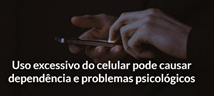
\includegraphics[width=.4\textwidth]{trigonometricas20}

\end{figure}

\begin{quote}

Dados mostram que $12\%$ dos americanos já desenvolveram dependência dos smartphones; psicólogo explica os riscos para a saúde mental.

A reportagem é de Giulia El Halabi, publicada por EcoDebate, 06-08-2019.


Quem nunca pegou o celular apenas para checar mensagens e passou dezenas de minutos - ou até mesmo algumas horas - vidrado na telinha? Esse comportamento cada vez mais comum pode se tornar um vício que já atinge 12\% dos americanos, segundo dados do \textit{Center for Internet and Technology Addiction}.

“O celular ativa continuamente o Sistema de Recompensa, estrutura do cérebro que recebe toda atividade prazerosa. Esse estímulo constante é o que gera dependência, em um processo similar à atuação de drogas ilícitas”, diz o psicólogo e professor do Centro Universitário Internacional Uninter, Ivo Carraro.

O uso abusivo dos smartphones pode gerar transtornos psíquicos, como ansiedade e, posteriormente, depressão. O transtorno já tem um nome: nomofobia, medo de ficar sem o celular. Longe do aparelho, o indivíduo fica ansioso, com a sensação de estar perdendo informações importantes, ou ainda excessivamente entediado.

Outro prejuízo é a dificuldade de sociabilização e isolamento. “Os humanos são seres de linguagem verbal e sociabilidade acentuadas. Quando se comunicam somente por mensagens, que são ‘mudas’, a palavra falada é eliminada e a inépcia social aumenta, agravando quadros depressivos”, explica o professor.

A exposição excessiva ao celular também pode causar insônia. Isso acontece porque a luz azul do aparelho ‘diz’ ao cérebro que ele deve ficar alerta. Assim, a produção de melatonina, o hormônio do sono, é inibida.

\flushright
(Fonte: \href{http://www.ihu.unisinos.br/78-noticias/591422-uso-excessivo-do-celular-pode-causar-dependencia-e-problemas-psicologicos}{Instituto Humanitas Unisinos})
\end{quote}

Como forma de contribuir com os usuários, as plataformas têm disponibilizado algumas ferramentas de registro de acesso aos ambientes mais acessados. Experimente olhar em seu smartphone, nas configurações, se há essa ferramenta - normalmente, o nome é \textit{bem estar digital}.

\begin{figure}[H]
\centering

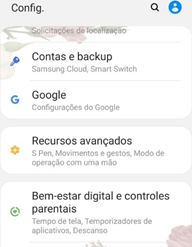
\includegraphics[width=.3\linewidth]{trigonometricas21}
\end{figure}

Por exemplo, alguns registros diários de uso de um aplicativo de mensagens bastante popular no smartphone de uma professora (observando o período de uma semana) estão exibidos a seguir. A primeira informação diz respeito ao número de mensagens recebidas e a segunda informação mostra quantas vezes o aplicativo foi aberto ao longo daquele dia. O dia 13 de agosto foi uma quinta-feira.


\begin{figure}[H]
\centering

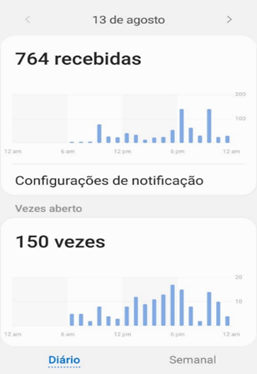
\includegraphics[height=.3\textheight]{trigonometricas22}
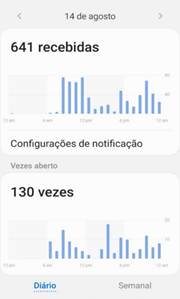
\includegraphics[height=.3\textheight]{trigonometricas23}
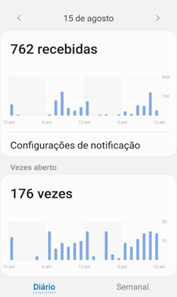
\includegraphics[height=.3\textheight]{trigonometricas24}
\end{figure}

\begin{figure}[H]
\centering

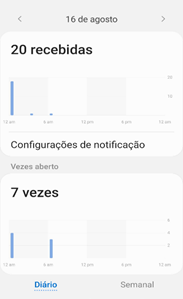
\includegraphics[height=.3\textheight]{trigonometricas25}
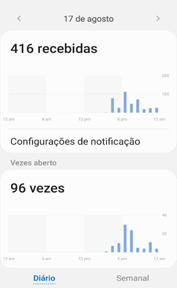
\includegraphics[height=.3\textheight]{trigonometricas26}
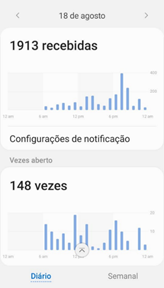
\includegraphics[height=.3\textheight]{trigonometricas27}
\end{figure}

\begin{figure}[H]
\centering

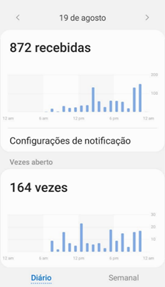
\includegraphics[height=.3\textheight]{trigonometricas28}
\end{figure}
\newpage

\begin{enumerate}
\item Preencha a tabela a seguir com os dados apresentados na figura anterior.

\begin{table}[H]
\centering

\scalebox{.8}
{
\begin{tabular}{|e{.2\linewidth}|e{.2\linewidth}|e{.2\linewidth}|}
\hline
\tcolor{Dia da Semana} & \tcolor{N\super{o} de mensagens recebidas} & \tcolor{N\super{o} de vezes que o aplicativo foi aberto} \tabularnewline
\hline
1 (qui) & & \tabularnewline
\hline
2 (sex) & & \tabularnewline
\hline
3 (sáb) & & \tabularnewline
\hline
4 (dom) & & \tabularnewline
\hline
5 (seg) & & \tabularnewline
\hline
6 (ter) & & \tabularnewline
\hline
7 (qua) & & \tabularnewline
\hline
\end{tabular}
}
\end{table}

\item Marque num plano cartesiano (físico ou digital) pontos $(x,y)$ correspondendo às duas primeiras colunas da tabela, onde $x$ representa o dia da semana e y o número de mensagens recebidas pela professora naquele dia. Em seguida, construa um segmento de reta ligando o ponto correspondente ao dia 1 ao ponto correspondendo ao dia 2, um segmento de reta ligando o ponto correspondente ao dia 2 ao ponto do dia 3 e assim sucessivamente até chegar ao ponto associado ao dia 7.
\item Faça o mesmo que foi pedido no item \titem{b)}, agora considerando que, nos pares $(x,y)$, $x$ representa o dia da semana e $y$ o número de vezes que para a quantidade de vezes em que a professora abre esse aplicativo.
\item Que observações você pode fazer sobre a rotina dessa professora?
\item As funções com domínio sendo o intervalo $[1,7]$ da reta e cujos gráficos foram esboçados nos itens \titem{b)} e \titem{c)} podem ser ditas periódicas? Se sim, justifique; se não, analise as fotos do enunciado de forma a descobrir ao menos algum padrão de regularidade no comportamento da rotina da professora que poderiam dar ideia de periodicidade.
\item Suponha que os mesmos dados de números de mensagens recebidas e de vezes que o aplicativo foi aberto sejam reproduzidos nos dias seguintes: no dia 8, a professora recebe o mesmo número de mensagens que no dia 1, no dia 9 ela recebe o mesmo número de mensagens que no dia 2 e assim sucessivamente (mesmo raciocínio para o número de vezes que o aplicativo foi aberto). As linhas poligonais construídas ligando pontos consecutivos, como feito nos itens \titem{b)} e \titem{c)}, agora representam gráficos de funções periódicas? Se sim, qual será o valor do período e da amplitude delas?
\item Se você ou alguém de sua família tiver um smartphone com essa função, veja que aplicativos aparecem com registro nessa ferramenta e que parâmetros são exibidos (tempo de tela, número de vezes em que o aplicativo é aberto, número de notificações, entre outros).
\item Colete os dados referentes a algum aplicativo de mensagens e anote, reproduzindo os passos \titem{a)}, \titem{b)}, \titem{c)} e \titem{d)}.

\end{enumerate}

\end{task}


\begin{knowledge}
\label{trig-knowledge1}
\vspace{-2\parskip}
\paragraph{O Som e as Ondas Sonoras}
O som é resultante de uma vibração, que se transmite em meios materiais de propagação, como sólidos, líquidos e gasosos.  Quando uma fonte sonora produz uma vibração, esta é transmitida a todo o meio material que a envolve e em todas as direções. Esta vibração é comunicada aos constituintes mais próximos da matéria, que sucessivamente a transmite aos constituintes seguintes através de choques entre eles.

A vibração de uma fonte sonora causa uma onda no meio de propagação. O som propaga-se por ondas invisíveis: as ondas sonoras ou acústicas. Portanto, o som pode ser descrito através de uma sequência de ondas sonoras, que são ondas de deslocamento, densidade e pressão que se propagam pelos meios compressíveis. Quando uma onda sonora se propaga através de qualquer gás, ocorrem várias compressões e rarefações de pequenos volumes do gás.

\begin{figure}[H]
\centering

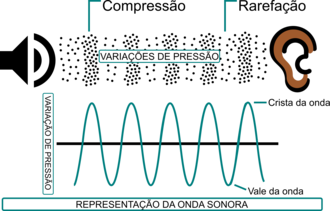
\includegraphics[width=.5\linewidth]{trigonometricas33}
\caption{Fonte: \href{https://pt.wikipedia.org/wiki/Som}{Wikipedia} }
\label{}
\end{figure}

Assista ao vídeo a seguir para compreender melhor o que são as ondas sonoras e como o som se propaga: \url{https://www.youtube.com/watch?v=sEa0dvnqrnw}

\begin{figure}[H]
\centering

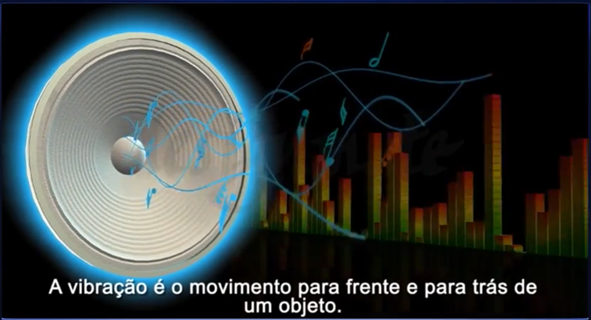
\includegraphics[width=.75\linewidth]{trigonometricas34}
\end{figure}

\needspace{5em}
As ondas sonoras mais simples são representadas por gráficos de um tipo muito específico de função periódica. Em estudos avançados de Física e Matemática constataram que toda onda sonora é gerada a partir de uma combinação dessas ondas sonoras mais simples, ou seja, de funções periódicas.

Podemos enxergar estas ondas? Há um equipamento muito \textit{utilizado} por profissionais da área de elétrica e eletrônica é o osciloscópio, que permite a visualização de formas de ondas eletromagnéticas. Esses dispositivos também são capazes de “ler”{} sinais sonoros, acoplando a eles um microfone.

Faça o \textit{download} em seu celular do aplicativo gratuito \textit{Oscilloscope}. Ele é capaz de captar os sons e reproduzir o que seriam as suas ondas sonoras correspondentes.

\begin{figure}[H]
\centering

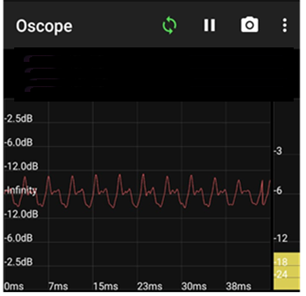
\includegraphics[width=.5\linewidth]{trigonometricas35}
\caption{O aplicativo Oscilloscope. Fonte: Os autore}
\label{}
\end{figure}

\begin{enumerate}
\item Capture com o aplicativo sons em diferentes volumes (clicando no ícone da câmera no topo à direita da tela é possível capturar a imagem da onda sonora). Qual é a diferença nas ondas geradas?
\item Capture com o aplicativo sons graves e agudos. Qual a diferença nas ondas geradas?
\item Procure gerar sons cujas ondas sonoras tenham trechos representados por um gráfico de funções periódicas como a da figura. Explore a relação entre a \textbf{amplitude} e o \textbf{período} da função associada a essa onda.

\end{enumerate}

\end{knowledge}



\needspace{15em}
\begin{knowledge}
\label{trig-knowledge2}


O eletrocardiograma (ECG) é um exame médico simples, indolor e rápido, levando em média 3 minutos para fazê-lo, no qual os impulsos elétricos do coração são amplificados e registrados. Em geral, um paciente faz um ECG quando há suspeita de doença cardíaca, mas ele também costuma ser feito como parte de exames físicos de rotina para pessoas de meia-idade e idosas, mesmo que elas não tenham nenhuma evidência de doença cardíaca.

Para realizar o ECG, um examinador coloca eletrodos (sensores redondos e pequenas que aderem à pele) nos braços, pernas e tórax da pessoa. Esses eletrodos medem a magnitude e a direção das correntes elétricas no coração durante cada batimento cardíaco. Os eletrodos são ligados por cabos a uma máquina que produz um registro (traçado) para cada eletrodo. Cada traço mostra a atividade elétrica do coração a partir de ângulos diferentes. No ECG são produzidos esses traços.

A figura a seguir ilustra as ondas associadas às atividades elétricas do coração. O batimento cardíaco começa com um impulso que ativa as câmaras superiores do coração (átrios). A onda P representa a ativação dos átrios. Em seguida, a corrente elétrica flui para as câmaras inferiores do coração (ventrículos). O trecho QRS representa a ativação dos ventrículos. A corrente elétrica, em seguida, espalha-se para trás, ao longo dos ventrículos no sentido oposto. Esta atividade é chamada onda de recuperação, representada pela onda T.



\begin{figure}[H]
\centering

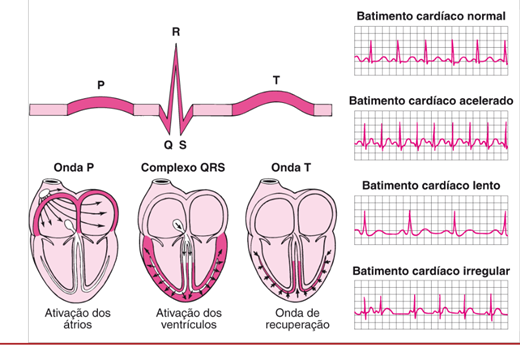
\includegraphics[width=.7\linewidth]{trigonometricas36}
\caption{Fonte: \href{https://www.msdmanuals.com/pt/casa/dist\%C3\%BArbios-do-cora\%C3\%A7\%C3\%A3o-e-dos-vasos-sangu\%C3\%ADneos/diagn\%C3\%B3stico-de-dist\%C3\%BArbios-do-cora\%C3\%A7\%C3\%A3o-e-dos-vasos-sangu\%C3\%ADneos/eletrocardiograma}{Manual MSD}}
\label{eletrocardiograma}
\end{figure}

Como a mecânica do coração se repete constantemente, a sistematização dessas ondas gera uma onda contínua que é impressa ao longo do exame. Em geral, esta onda é representada pelo gráfico de uma função periódica. Quando isto não ocorre, tem-se um indício de arritmia cardíaca, ou seja, um batimento cardíaco irregular.
Mesmo que a onda impressa seja representada por uma função periódica, nem sempre o coração do paciente estará sadio: o batimento cardíaco pode estar mais acelerado ou mais lento do que o normal para uma situação de repouso, o fica visível através do período da função periódica associada ser muito baixo ou muito alto, comparado ao de um batimento cardíaco normal (vide \hyperref[eletrocardiograma]{figura \ref{eletrocardiograma}}).


\end{knowledge}
\clearpage

\def\currentcolor{session1}
\begin{objectives}{Cobrindo circunferências com seus raios}
{
\begin{itemize}
\item Introduzir ao aluno uma nova forma de se mensurar ângulos na circunferência, tomando como unidade de medida, um arco de medida igual ao raio da mesma.
\end{itemize}
}{1}{1}
\end{objectives}
\begin{sugestions}{Cobrindo circunferências com seus raios}
{
Os itens \titem{b)} e \titem{c)} pretendem convencer o aluno de que, independente do tamanho da circunferência, essa nova unidade de medida corresponde a um mesmo valor em graus, valor este aproximadamente $57^{\circ}$, o que permitirá estabelecer uma primeira correspondência entre essas duas formas de medir ângulos. 

Ao longo da atividade, o aluno poderá adotar diferentes estratégias, como dividir os $360$ graus de uma volta inteira pela medida do ângulo central ou ainda ir colando outros pedaços de barbante sobre o contorno da circunferência para verificar. Cuide para que eles adotem as próprias estratégias e que compartilhem uns com os outros. Nesta atividade, caso prefira, pode-se também desenhar diferentes circunferências usando o compasso, substituindo os objetos redondos.
}{1}{1}
\end{sugestions}
\begin{answer}{Cobrindo circunferências com seus raios}
{
\begin{enumerate}
\item Arco
\item A medida do ângulo será, o valor em graus de 1 radiano,
isto é, aproximadamente $57^{\circ}$.
\item Os valores serão muito próximos, com pequenas variações em virtude de erros de medição.
\item $6$
\end{enumerate}
}{1}
\end{answer}
\clearmargin
\begin{answer}{Cobrindo circunferências com seus raios}
{
	\begin{enumerate}\setcounter{enumi}{4}
	\item Não é possível cobrir a circunferência com uma quantidade inteira de raios, visto que o seu comprimento é o resultado da multiplicação do raio por um número irracional: $C =(2\pi)r\approx6{,}28r = 6r + 0{,}28r$.

	Logo, a parte que fica descoberta, referida no enunciado, corresponderá a um valor aproximado de 0,28 vezes a medida do raio. 
	\end{enumerate}
}{1}
\end{answer}
\begin{objectives}{Ângulos e Arcos de Circunferência no GeoGebra}
{
\begin{itemize}
\item Apresentar ao aluno a definição de radiano, levando-o a relacionar essa nova unidade de medida de ângulos com a medida do comprimento do arco de qualquer circunferência delimitado por ele.
\end{itemize}
}{1}{2}
\end{objectives}
\begin{sugestions}{Ângulos e Arcos de Circunferência no GeoGebra}
{
No caso em que o raio da circunferência for $1$, o aluno perceberá que a medida do ângulo em radianos será exatamente a medida do comprimento do arco da circunferência unitária delimitado por ele.

Você poderá encontrar essa construção pronta no link \url{https://www.geogebra.org/m/xfqkgymy}. Recomenda-se, no entanto, que incentive seus alunos a construir. O passo a passo poderá ser acessado abrindo-se o PROTOCOLO da construção no menu principal, submenu EXIBIR.
}{1}{2}
\end{sugestions}
\begin{answer}{Ângulos e Arcos de Circunferência no GeoGebra}
{
\begin{enumerate}
\item O valor de $k$ não se altera. 
\item $k$ variará de $0$ (quando o $C$ estiver sobre $B$) até aproximadamente $6{,}28$ (quando ele estiver próximo de completar uma volta em torno de $B$).
\item A razão $k$ independe da medida a do raio da
circunferência.
\item Os valores são iguais.
\item O valor da razão $k$ independe da medida a do raio da
circunferência.
\item A medida $k$ será exatamente igual à medida do comprimento do arco $BC$ e também igual à medida do ângulo $B\hat{A}C$ na unidade “radianos”.
\end{enumerate}
}{1}
\end{answer}
\explore{O Radiano}
\label{trig-exp2}

\begin{task}{Cobrindo circunferências com seus raios}
\label{trig-ativ7}

Vamos propor agora uma atividade para você fazer com os seus colegas na sala de aula. Se organizem em duplas ou grupos e sigam os passos a seguir:
\begin{enumerate}[label=\titem{\arabic*.}, wide, left=0pt]
\item Providencie objetos redondos que você possa levar para a sala de aula (rodinhas de carrinho de brinquedo, copos, garrafas, tampas de potes e panela, etc);
\item Use esses objetos para desenhar circunferências numa folha suficientemente grande, contornando-as com um lápis;
\item Determine o centro dessas circunferências. Para isso, tome três pontos sobre a circunferência e trace as mediatrizes de dois segmentos distintos com extremidades nesses pontos. O encontro entre essas mediatrizes é o centro da circunferência;
\item Meça o raio dessas circunferências;
\item Para cada uma das circunferências, corte um pedaço de barbante que tenha essa medida e ajuste-o sobre a circunferência, colando-o no papel.
\end{enumerate}

\begin{figure}[H]
\centering

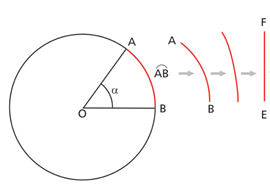
\includegraphics[width=.4\linewidth]{trigonometricas37}
\end{figure}

\begin{enumerate}
\item Qual o nome do objeto geométrico equivalente à parte das circunferências coberta pelo barbante?
\item A partir de cada extremidade dos pedaços de barbante colados sobre cada circunferência, trace dois segmentos que unam as extremidades dos barbantes ao centro de cada circunferência. Meça os ângulos centrais que ficam assim determinados em cada circunferência. Qual a medida do ângulo central encontrada em cada uma delas?
\item Compare a sua resposta do item \titem{c)} com as de outras duplas ou grupos de sua turma. Há algo que você consegue notar nos valores obtidos?
\item Quantas vezes o raio da circunferência cabe no comprimento da mesma?
\item É possível cobrir toda a circunferência com uma quantidade inteira de segmentos com medida igual à do seu raio? Se sim, diga quantos segmentos são necessários; se não, estime o valor da fração do raio do círculo correspondente ao pedacinho que ficou descoberto.
\end{enumerate}
\end{task}


\begin{task}{Ângulos e Arcos de Circunferência no GeoGebra}
\label{trig-ativ8}

Abra o GeoGebra e crie um controle deslizante a variando de $0$ a $10$. Crie o ponto $A$ e construa uma circunferência de centro $A$ com raio $a$. Tome um ponto $B$ sobre a circunferência e construa o segmento $AB$, cujo comprimento ficará registrado na janela da álgebra. Agora, crie um ponto $C$ sobre a circunferência e construa o (menor) arco circular de centro $A$ e extremidades $C$ e $B$, cujo comprimento ficará indicado na Janela da Álgebra.

\begin{enumerate}
\item Usando o GeoGebra, determine a razão $k$ entre o comprimento do arco $BC$ e o raio da circunferência. Movimente o controle deslizante do parâmetro $a$. O que você observa em relação ao valor de $k$?
\item Altere a medida do comprimento do arco $BC$ movendo o ponto $C$ ao longo da circunferência. Qual o intervalo de variação da razão $k$?
\item Movimente $C$ de forma que o comprimento do arco $BC$ fique igual ao comprimento do raio da circunferência. Qual o valor da razão $k$ nesse caso? Movimente o controle deslizante novamente e registre o que você observa.
\item Construa e meça o ângulo central ${B\hat{A}C}$ e modifique a unidade de medida para \textit{“radianos}”. Movimente o ponto $C$ sobre a circunferência. O que você pode observar em relação ao valor de $k$ e a medida do ângulo central da circunferência em radianos?
\item Movimente o controle deslizante a e observe o valor da razão $k$.
\item Reproduza a atividade, agora com uma circunferência que tenha um raio fixo e igual a $1$. Comente como ficam os valores de $k$ e do ângulo ${B\hat{A}C}$.
\end{enumerate}

\end{task}

\arrange{O Radiano}
\label{trig-arg2}

Na atividade \hyperref[trig-ativ7]{Cobrindo circunferências com seus raios}, você pôde observar que, mesmo que variemos o raio da circunferência, o ângulo central (com vértice no centro da circunferência) determinado por um arco da circunferência que tem comprimento igual à medida do raio é o mesmo. Além disso, também foi possível verificar que cabem sobre a linha da circunferência $6$ “pedaços”{} inteiros de barbante com o comprimento igual ao raio da circunferência, faltando um arco cujo comprimento é menor que o comprimento do raio da circunferência em questão.

Na segunda atividade - \hyperref[trig-ativ8]{Ângulos e Arcos de Circunferência no GeoGebra} - você pôde observar que a razão entre o comprimento de um arco qualquer na circunferência e o seu raio varia entre $0$ e valores menores que $6{,}3$ - ou seja, isso indica que o raio da circunferência “cabe”{} sobre o seu contorno pouco mais de $6$ vezes inteiras. Mas exatamente, quantas vezes será que o raio de uma circunferência cabe sobre o seu contorno?

Para determinar esse valor, vamos nos lembrar que, no Ensino Fundamental, você aprendeu que o comprimento $C$ de uma circunferência de raio $r$ é $C=2\pi r$. A operação que nos permite verificar quantas vezes uma grandeza “cabe”{} em outra de mesma natureza é a divisão; então, como queremos verificar quantas vezes o raio cabe na circunferência, vamos dividir o comprimento da circunferência pelo raio. Temos então:
\begin{equation*}
\frac{2\pi r}{r}=2\pi.
\end{equation*}

Isso quer dizer que o raio de uma circunferência cabe sobre o seu contorno $2\pi$ vezes - o que é coerente com o que encontramos na atividade \hyperref[trig-ativ8]{Ângulos e Arcos de Circunferência no GeoGebra} ou ainda na atividade \hyperref[trig-ativ7]{Cobrindo circunferências com seus raios}. Tomando para   o valor aproximado de $3{,}14$ (lembrando que esse é uma aproximação, na verdade,$\pi$ é um número irracional!), encontramos $2\cdot\pi\cong2\cdot3{,}14=6{,}28$, ou seja, pouco menos do que $6,3$. E observe: esse resultado não depende do raio da circunferência!

O que estamos fazendo aqui é uma ação de \textbf{\textit{medir} arcos de circunferências} (e seus respectivos ângulos centrais), mas usando o \textbf{\textit{raio da circunferência como unidade de medida}} e não os já conhecidos graus, que remetem ao ângulo central da circunferência que determina o arco que desejamos medir. A unidade de medida de arcos provenientes dessa ação é o \textit{radiano}. Escrevemos $\rad$ para denotar esta nova unidade medida. Então, o radiano é uma unidade de medida de arcos tal que $2\pi \rad$ é a medida do arco que cobre completamente a circunferência, sem sobreposições. Assim sendo, podemos estabelecer uma correspondência entre a nossa já conhecida unidade de medida de arcos em graus e a nova unidade radianos: como o arco de uma volta inteira mede, em graus, $360^{\circ}$, então podemos escrever que:
\begin{equation*}
360^{\circ}=2\pi\rad
\end{equation*}

Dividindo os dois lados da igualdade por $2$, teremos de forma mais simplificada que $180^{\circ}=\pi \mathrm{rad}$. Podemos usar essa relação para poder ler a medida de qualquer arco em graus ou em radianos, convertendo de uma à outra sempre que necessário. Em particular, a medida em graus de um arco cujo comprimento é de $1\rad$ (um arco cujo comprimento é exatamente $1$ raio) pode ser determinada dividindo-se ambos os termos na igualdade acima por $\pi$:
\begin{equation*}
180^{\circ}=\pi \rad\therefore\frac{180^{\circ}}{\pi}=\frac{\pi}{\pi} \rad\therefore1 \rad=\frac{180^{\circ}}{\pi}
\end{equation*}

\begin{observation}{}
É interessante observar que, ao tratar dessas duas unidades de medida, estamos percebendo duas características importantes do arco: a medida do ângulo central que o determina sobre a circunferência e a quantidade de vezes que o raio da circunferência cabe sobre aquele arco. Quando desejamos nos remeter à medida do arco correspondente ao ângulo central, a medida em graus é a mais esclarecedora; por outro lado, quando desejamos indicar quantos raios cabem no comprimento do arco, então a medida em radianos é a mais adequada. E note que podemos facilmente transitar de uma à outra a partir do uso da relação $180^{\circ}=\pi\rad$.
\end{observation}


Para podermos ter uma boa ideia do que estamos tratando, vamos considerar dois relógios analógicos: o relógio de Meca, dito o maior do mundo, que tem $4$ faces com $43$ metros de diâmetro em cada face e um relógio de pulso comum, que tem em torno de $3$ cm de diâmetro.

\begin{figure}[H]
\centering

\begin{minipage}{.45\linewidth}
\begin{figure}[H]
\centering

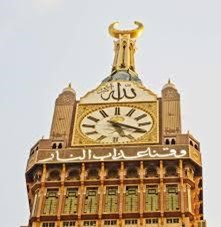
\includegraphics[height=175bp]{trigonometricas38}
\caption{Fonte: \href{https://gigantesdomundo.blogspot.com/2012/11/o-maior-relogio-do-mundo.html}{Gigantes do Mundo}}
\label{}
\end{figure}
\end{minipage}
\hspace{2em}
\begin{minipage}{.45\linewidth}
\begin{figure}[H]
\centering

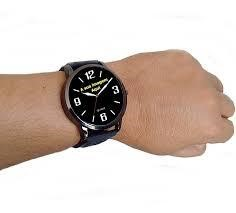
\includegraphics[height=175bp]{trigonometricas39}
\caption{Fonte: \href{https://produto.mercadolivre.com.br/MLB-1160291326-relogio-pulso-personalizado-com-foto-imagem-logo-promoco-_JM}{Mercado Livre}}
\label{}
\end{figure}
\end{minipage}
\end{figure}

Vamos considerar que os dois relógios estão marcando corretamente as horas, sem atrasar nem adiantar, e que ambos estejam marcando exatamente $3$ h - ou seja, o ponteiro pequeno aponta para o número $3$ e o ponteiro grande para o número $12$. Vamos observar os arcos determinados nos dois relógios pelas semirretas que têm origem no centro dos relógios e que passam pelo $12$ e pelo $3$, respectivamente.

\begin{figure}[H]
\centering

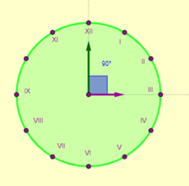
\includegraphics[width=.35\linewidth]{trigonometricas40}
\hspace{2em}
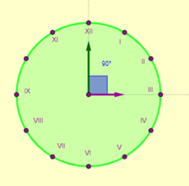
\includegraphics[width=.35\linewidth]{trigonometricas40}
\caption{Disponível em: \url{https://www.geogebra.org/m/gTMSvJTB}}
\label{}
\end{figure}

Nos dois relógios, a medida do arco de extremidades $C$ e $E$ tem a medida de $90^{\circ}$ - essa é a medida angular desse arco, pois remete à medida do ângulo central de vértice $D$ que mede também $90^{\circ}$. Por outro lado, evidentemente, a medida do \textit{comprimento} do arco de extremidades $C$ e $E$ é diferente nos dois relógios: no relógio de pulso, de diâmetro $3$ cm (e raio $1{,}5$ cm), o comprimento desse arco será de $C=\frac{(2\cdot\pi\cdot1{,}5}{4}=\frac{3}{4}\pi$ cm, ou seja, aproximadamente $2{,}35$ cm . Por outro lado, no relógio de Meca com $43$ m de diâmetro, temos $21{,}5\text{ m } = 2150$ cm de raio e então o arco $CE$ terá comprimento  
\begin{equation*}
C=\dfrac{2\cdot\pi\cdot2.150}{4}=1.075\pi\cong3375{,}5\text{ cm}.
\end{equation*}
Porém, a medida em radianos do arco $CE$ em ambos os relógios será a mesma! Lembre-se: medir um arco em radianos significa que queremos saber quantas vezes o raio da circunferência cabe naquele arco. No relógio de pulso, a medida em radianos de CE será o quociente entre a medida do seu comprimento pelo raio da circunferência, isto é, $\dfrac{\frac{3}{4}\pi}{1{,}5}=\frac{\pi}{2}\rad$, enquanto que no relógio de Meca será $\dfrac{1.075\pi}{2.150}=\dfrac{\pi}{2}\rad$. Repare que, segundo a regra de conversão $108^{\circ}=\pi\rad$, estabelecida entre graus e radianos dividindo ambos os lados da igualdade por $2$, obtemos $90^{\circ}=\frac{\pi}{2}\rad$. Em particular, arcos correspondendo a ângulos retos medem $\frac{\pi}{2}\rad$.

\clearpage
\def\currentcolor{session2}
\begin{objectives}{Medindo ângulos centrais em nosso planeta}
{
\begin{itemize}
\item Medir empiricamente arcos e ângulos
\item Usar ferramentas tecnológicas no trabalho com arcos e ângulo
\end{itemize}
}{1}{2}
\end{objectives}
\clearmargin
\begin{answer}{Medindo ângulos centrais em nosso planeta}
{
\begin{enumerate}
\item Aproximadamente $340$ km.
\item Aproximadamente $0{,}053\rad$.
\item Valores dependerão das escolhas dos alunos.
\end{enumerate}
}{1}
\end{answer}
\practice{O Radiano}
\label{trig-prac2}

\begin{task}{Medindo ângulos centrais em nosso planeta}
\label{trig-ativ9}

Um dos resultados mais fascinantes que já existiram na História da Matemática é decorrente do experimento realizado pelo matemático e astrônomo grego Eratóstenes. Estudando o comportamento das sombras de varetas nas cidades Alexandria e Syene (Assuã, nos dias atuais) ao meio dia, ele não só conseguiu perceber que a superfície da Terra não era plana como conseguiu calcular, com uma precisão surpreendente, o comprimento de uma volta completa ao redor da Terra!

Eratóstenes sabia que a distância entre as cidades de Alexandria e Syene era aproximadamente igual a $800$ km. Percebeu também que ao meio dia, o sol estava a pino em Syene de forma que nesse horário, podia-se ver o sol completamente refletido no interior do poço. Além disso, às $12$ h, nenhuma sombra era formada pelas colunas daquela cidade. O mesmo não ocorria em Alexandria: ao meio dia, uma vareta colocada de pé no chão apresentava uma sombra substancial e com ela, Eratóstenes conseguiu provar que o arco sobre a superfície da Terra, que compreende as cidades de Alexandria e Assuã media cerca de $\frac{\pi}{25}\rad$ ($7{,}2$ graus) e que corresponde ao ângulo central $\hat{A}$ da \hyperref[zenite]{figura \ref{zenite}}:

\begin{figure}[H]
\centering

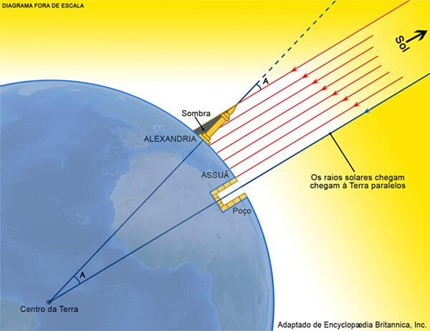
\includegraphics[width=.65\linewidth]{trigonometricas42}
\caption{Costa, J. R. V. Eratóstenes e a circunferência da Terra. \href{https://www.zenite.nu/eratostenes-e-a-circunferencia-da-terra/}{Astronomia no Zênite}, jul 2000.}
\label{zenite}
\end{figure}

Eratóstenes utilizou a seguinte regra de três para calcular o comprimento de uma volta completa ao redor da Terra:


\begin{equation*}
\begin{array}{ccc}
\frac{\pi}{25} \rad & \adjustbox{valign=c}{\tikz \draw (0,0) -- (1.5,0);} & 800 \text{ km} \\
2\pi\rad & \adjustbox{valign=c}{\tikz \draw (0,0) -- (1.5,0);} & C 
\end{array}
\end{equation*}

Resolvendo a regra de três, obtemos $C = 40.000$ km. Utilizando instrumentos tecnológicos muito mais avançados dos quais dispunha Eratóstenes, hoje se sabe que o comprimento de uma volta completa na Terra é de $40.072$ km, ou seja, o erro de cálculo do matemático grego foi de menos de $100$ km! O vídeo a seguir, apresenta parte de um episódio famosa série Cosmos, e narra com mais detalhes a ideia do experimento de Eratóstenes.

\begin{figure}[H]
\centering

\includegraphics[width=.5\linewidth]{trigonometricas43}

\caption{Acesse pelo link: \url{https://www.youtube.com/watch?v=fu9Z7YuXLVE}}
\end{figure}

Vamos utilizar o raciocínio de Eratóstenes, com o auxílio do Google Earth para medir arcos em graus e radianos, limitados por duas cidades brasileiras! Baixe e instale no seu smartphone o aplicativo Google Earth.


\begin{figure}[H]
\centering

\includegraphics[height=.3\textheight]{trigonometricas44}
\end{figure}

\begin{enumerate}
\item Use a ferramenta medir para encontrar uma aproximação para distância, ao longo do globo terrestre, entre as capitais Rio de Janeiro e Belo Horizonte.
\item Usando o fato que uma volta completa na Terra tem $40.072$ km, determine a medida aproximada do valor do arco (em radianos) sobre a superfície da Terra que liga as duas capitais do item \titem{a)}.
\item Reproduza os itens \titem{a)} e \titem{b)} para a cidade onde você mora e qualquer outra cidade de sua escolha no Brasil.
\end{enumerate}
\end{task}

\cleardoublepage
\def\currentcolor{session1}
\begin{objectives}{Carrinho VertiGo}
{
\begin{itemize}
\item Introduzir a ideia e a construção da Função de Euler,
\item Estabelecer a relação entre números reais e pontos de uma circunferência unitária.
\end{itemize}
}{1}{1}
\end{objectives}
\begin{sugestions}{Carrinho VertiGo}
{
\begin{itemize}
\item Sugerimos ao professor orientar os alunos, se necessário, a observarem que uma distância vertical de comprimento “$a$”{} percorrida pelo carrinho se reflete na posição do selo, o qual se moverá ao longo da roda percorrendo um arco de circunferência de mesmo comprimento “$a$”.
\item  O uso de objetos redondos e barbante utilizados na atividade “Cobrindo circunferências com seus raios”{} pode ajuda-los nessa percepção.
\end{itemize}
}{1}{1}
\end{sugestions}
\clearmargin
\marginpar{\vspace{.5em}}
\begin{answer}{Carrinho VertiGo}
{
 \begin{enumerate}
 \item A posição do selo referente às distâncias $0, 1, 2, \frac{3}{2}, \frac{\pi}{2}, \pi, \frac{3\pi}{2}$ e $7$ dm estão representadas  no desenho abaixo respectivamente pelos pontos $A_1, A_2, A_3, A_4, A_5, A_6, A_7\text{ e }A_8$. A posição referente às distâncias $2\pi$ e $4\pi$ dm é mesma do ponto $A_1$

 \begin{figure}[H]
 \centering
 
 \includegraphics[width=.4\linewidth]{trigonometricas47}
 \end{figure}
 \item Basta refletir os pontos obtidos no item \titem{a)} relativamente à reta horizontal que passa pelo centro da circunferência e o ponto $A_1$.
 \end{enumerate}
}{1}
\end{answer}
\begin{objectives}{"Abraçando"{} um círculo com uma reta}
{
\begin{itemize}
\item Construir, mais abstratamente em relação à atividade anterior, a sobrejeção da reta sobre a circunferência unitária dada pela função de Euler.
\end{itemize}
}{1}{2}
\end{objectives}
\begin{sugestions}{"Abraçando"{} um círculo com uma reta}
{
Repare que, por enquanto, não estamos preocupados com o sistema de coordenadas do plano que contém a circunferência. Estas coordenadas serão consideradas na próxima seção para formalizar o conceito de seno e cosseno de um número real. Neste momento, o importante é o aluno perceber como fica a posição dos números reais sobre a circunferência unitária após o “enrolar”{} da reta sobre a circunferência.
}{1}{2}
\end{sugestions}
\clearmargin
\begin{answer}{"Abraçando"{} um círculo com uma reta}
{
\begin{enumerate}
\item Apenas um ponto ficará coberto por cada número real.
\item A cada ponto da circunferência estarão associados infinitos números reais.
\item A cada arco de volta inteira descrito a partir do ponto $A$ teremos outros pontos da reta que irão se sobrepor em $A$, logo, esses pontos correspondem aos números reais $1 + 2k\pi$, onde que $k$ é um inteiro qualquer. Portanto, o primeiro número positivo após o $1$ cuja posição após o enrolar da reta será o mesmo ponto $A$ é $1 + 2\pi$, enquanto o primeiro número negativo a ser associado a $A$ será $1 - 2\pi$.
\item O ponto em que o número real $5$ está alocado encontra-se no 4º quadrante, visto que está entre $\frac{3\pi}{2}$ e $2\pi$; analogamente, o real $-5$ está no $1$\super{o} quadrante. O menor arco tem comprimento igual a $2\cdot|2\pi-5|$ o que equivale a, aproximadamente, $2{,}5$ unidades de comprimento. Outra maneira de se chegar ao resultado é percebendo que o comprimento do intervalo $[-5,5]$ é $10$, portanto, menor que o comprimento da circunferência de raio $2$, que é $4\pi$ . Portanto, a transformação que enrola o intervalo na circunferência determinará um arco de $10$ unidades e o arco complementar medirá $4\pi − 10$

\begin{figure}[H]
\centering

\includegraphics[width=.5\linewidth]{trigonometricas49}
\end{figure}
\end{enumerate}
}{1}
\end{answer}
\def\currentcolor{session4}
\begin{texto}
{
	\paragraph{Objetivo geral da seção}
	Estabelecer correspondências entre números reais e pontos de um círculo, de forma a motivar a compreensão da ideia de círculo trigonométrico e da função de Euler.
}
\end{texto}
\explore{Círculo Trigonométrico e a Função de Euler}
\label{trig-exp3}
\footnote{nota da diagramação: título muito grande}

\begin{task}{Carrinho VertiGo}
\label{trig-ativ10}

\begin{quote}

Pesquisadores da Disney Research, em parceria com o Instituto Federal de Tecnologia de Zurique, demonstraram esta semana um carrinho de quatro rodas capaz de escalar paredes e andar normalmente em superfícies verticais.
À primeira vista, parece um brinquedo, mas, segundo os criadores, a tecnologia pode ampliar os limites de exploração para equipamentos robóticos. Batizado como VertiGo, o carrinho é “capaz de mover em uma parede rapidamente e com agilidade”, informam os pesquisadores. Para realizar a façanha, ele possui duas hélices propulsoras móveis que fornecem o impulso necessário para o início da escalada e, depois, mantém o VertiGo junto à parede.”

\flushright
Fonte: \href{https://gizmodo.uol.com.br/o-novo-robo-da-disney-escala-paredes-como-uma-lagartixa/}{Gizmodo}
\end{quote}


\begin{figure}[H]
\centering

\includegraphics[width=.7\linewidth]{trigonometricas45}
\end{figure}

Neste link é possível ver o VertiGo em ação: \url{https://www.youtube.com/watch?v=KRYT2kYbgo4}


Suponha que foi colado um pequeno selo em uma das rodas do VertiGo. O carrinho começará a descer em um paredão vertical bem alto, seguindo um caminho reto e paralelo ao paredão. Ele começa o movimento “colado”{} ao paredão, quando o selo está em contato com o mesmo. Conforme o carrinho vai descendo, o selo se movimenta conforme o giro da roda. A figura abaixo ilustra o movimento realizado por essa roda ao descer o paredão e os pontos $A_1$, $A_2$ e $A_3$ ilustram posições do selo ao longo do movimento. Suponha que o raio da roda seja de $1$ dm

\begin{figure}[H]
\centering

\includegraphics[width=.375\linewidth]{trigonometricas46}
\caption{Fonte: Adaptado de \cite{ekici2010}}
\label{trigonometrica46}
\end{figure}

\begin{enumerate}
\item Indique a posição do selo na circunferência da roda quando o VertiGo tiver descido as seguinte distâncias:

$0\text{ dm}, 1\text{ dm}, 2\text{ dm}, \frac{3}{2}\text{ dm}, \frac{\pi}{2}\text{ dm}, \pi\text{ dm}, 3\pi\text{ dm}, 2\pi\text{ dm}, 7\text{ dm}, 4\text{ dm}$
\item Suponha que, do ponto de repouso do VertiGo, agora ele irá \textbf{subir} parte do paredão. Usando a mesma vista lateral dada pela \fref{trigonometrica46}, qual será a posição do sela para as mesmas medidas do item \titem{a)}?
\end{enumerate}


\end{task}

\begin{task}{"Abraçando"{} um círculo com uma reta}
\label{trig-ativ11}

Observe a imagem a seguir e responda às perguntas:
\begin{figure}[H]
\centering

\includegraphics[width=.9\linewidth]{trigonometricas48}
\end{figure}

\begin{enumerate}
\item Quantos pontos da circunferência estarão “cobertos”{} pelo número real $1$?
\item A cada ponto da circunferência, quantos números reais ficam associados?
\item Considerando o ponto $A$ na circunferência sobre o qual encontra-se o número real $1$. Qual o próximo número real positivo que também estará localizado em $A$? E qual será o primeiro número negativo associado a $A$?
\item Se reproduzimos a construção exibida acima usando, em lugar da reta real, o intervalo $[-5,5]$ em uma circunferência de raio $2$, tangenciando esta circunferência no ponto $0$ do intervalo, qual será a medida do menor arco encontrado entre os pontos da circunferência associados a $-5$ e $5$?
\end{enumerate}
\end{task}

\arrange{Círculo Trigonométrico e a Função de Euler}
\label{trig-arg3}

Nas atividades \hyperref[trig-ativ10]{\textit{Carrinho VertiGo}} e \hyperref[trig-ativ11]{\textit{"Abraçando"{}  um círculo com uma reta}} você aprendeu que é possível associar números reais a pontos de uma circunferência de raio $1$. Considere que no plano tem-se um sistema de coordenadas cartesianas, no qual $C^1$ representa a circunferência de centro na origem e raio $1$. Repare que $A = (1,0)\in C^1$ pois esse ponto tem distância $1$ para a origem. A \textit{Função de Euler}, que será denotada pela letra $E$, é uma ferramenta matemática que permite corresponder formalmente qualquer número real a um ponto de $C^1$. Definimos $E:R\to C^1$,  da seguinte maneira: dado qualquer número real $t > 0$, construiremos um arco de comprimento $|t|$ na circunferência  $C^1$, com uma de suas extremidades no ponto $A$ e a outra extremidade num ponto $E(t)$ percorrendo $C^1$ no sentido contrário aos ponteiros do relógio (anti-horário). Se $t < 0$ fazemos o mesmo procedimento, porém percorrendo a circunferência em sentido horário. Finalmente, se $t = 0$, definimos $E(0) = A$.

\begin{minipage}{.45\linewidth}
\begin{figure}[H]
\centering

\includegraphics[width=\linewidth]{trigonometricas50}
\caption{$E(t)$ para $t>0$}
\label{}
\end{figure}
\end{minipage}
\begin{minipage}{.45\linewidth}
\begin{figure}[H]
\centering

\includegraphics[width=\linewidth]{trigonometricas51}
\caption{$E(t) \text{ para } $t<0}
\label{}
\end{figure}
\end{minipage}

Repare que eventualmente, o valor de $|t|$ pode ser maior que a medida do comprimento da circunferência $C^1$ . Se isto ocorrer, o arco de extremidades $A$ e $E(t)$ será construído de forma que se percorrerá a linha da circunferência dando mais que uma volta em torno da origem do plano cartesiano: por exemplo, se $t=-4\pi$, então, como $C^1$ tem comprimento $2\pi\cdot1=2\pi$, $E(t)$ será obtido construindo um arco partindo de $A$ e fazendo-se um percurso de $|-4\pi |=4\pi$ unidades ao longo de $C^1$ no sentido horário, o que corresponde exatamente a dar umas voltas completas na circunferência, finalizando o percurso em $A$. Logo, $E(-4\pi)=A$. Por outro lado, para encontrar $E(7\pi)$, começamos percorrendo $7\pi$ unidades de comprimento ao longo de $C^1$ , mas agora em sentido anti-horário. O percurso termina no ponto $(-1,0)$ pois $7\pi=3\cdot(2\pi)+\pi$, o que corresponde a dar $3$ voltas em $C^1$ a partir de $A$ no sentido anti-horário e depois percorrer mais meia volta. Logo, $E(7\pi) = (-1,0)$.

A dinâmica do cálculo de imagens pela Função de Euler motiva a definição do \textbf{círculo (ou ciclo) trigonométrico} que consiste essencialmente em três ingredientes: circunferência de raio unitário, sistema de eixos cartesianos e orientação. Vamos falar um pouco sobre cada um deles.

\paragraph{Circunferência de raio unitário}

Vimos na seção “O radiano”{} que a medida de um arco em radianos indica a quantidade de vezes que o raio da circunferência na qual o arco está contido “cabe”{} sobre esse arco, ou seja, a medida angular do arco é o resultado da razão entre o comprimento do arco e o raio da circunferência que contém esse arco. Lembre-se que a medida em radianos de um arco em uma circunferência é calculada através do quociente entre o comprimento do arco e o raio. Esse cálculo fica mais fácil quando o raio mede $1$ unidade, o que nos dá uma equivalência direta entre $C^1$ o comprimento do arco e a medida angular em radianos desse arco. Então, considerar arcos em uma circunferência de raio unitário traz a vantagem de termos medidas de mesmo valor para as medidas angular (relacionada ao ângulo central, à abertura do arco) e linear (relacionada ao comprimento do arco).

\paragraph{Sistema de eixos cartesianos}

O sistema de eixos cartesianos é o sistema com um par de retas perpendiculares orientadas e graduadas, em cuja interseção se localiza o ponto de coordenadas $(0,0)$, denominado \textit{origem do sistema de eixos cartesianos}. A associação entre o sistema de eixos cartesianos e a circunferência de raio unitário nos possibilitará associar coordenadas aos pontos sobre a circunferência.

\paragraph{Orientação}

A circunferência que representa o círculo trigonométrico é orientada, o que indica que há um ponto tomado como origem e uma orientação que atribui um sentido positivo (sentido anti-horário) e um sentido negativo (sentido horário) para os arcos tomados sobre essa circunferência. A seguir podemos ver uma imagem que representa o círculo trigonométrico e seus pontos notáveis.

\begin{figure}[H]
\centering

\includegraphics[width=.75\linewidth]{trigonometricas52}
\end{figure}

A partir do momento em que conseguimos associar comprimentos com arcos no círculo trigonométrico, já podemos pensar em associar números reais ao círculo trigonométrico. Um arco de comprimento 2, por exemplo, seria um arco de $2 \rad$ --- mas onde ele começa? Onde acaba? E o arco de $-2\rad$, onde o marcamos?

Determinar a origem do círculo trigonométrico como sendo o ponto $(1,0)$ e estabelecer o sentido positivo como o anti-horário e negativo como o horário torna essa missão mais simples. Um arco de $2\rad$ tem origem em $(1,0)$ e estende-se por um comprimento igual a $2$ unidades no sentido anti-horário. E o arco de $-2 \rad$? Esse arco também tem origem em $(1,0)$, mas estende-se com comprimento $2$, mas no sentido horário do círculo, pois é negativo. Na figura a seguir vemos esses arcos.

\begin{figure}[H]
\centering

\includegraphics[width=.39\linewidth]{trigonometricas53}
\end{figure}

Por sua vez, o número zero será associado a um “arco”{} que consiste em um único ponto, a saber, a origem $(1,0)$ do círculo trigonométrico.

Vamos generalizar essas ideias? Na figura a seguir, o ângulo ${B\hat{O}A}$ tem medida $\alpha$, em graus. A \textit{medida} do arco $AB$ será  $\frac{\alpha}{360^{\circ}}\cdot2\pi\rad$. A razão $\frac{\alpha}{360^{\circ}}$ indica que parte da circunferência inteira (de comprimento $2\pi$ pois o raio é $1$) é ocupada pelo arco $AB$. Se $\alpha$ é dado em radianos, então a medida do arco $AB$ será, da mesma forma que vimos acima, $\frac{\alpha}{2\pi}\cdot2\pi\rad$ , ou seja, é $\alpha$.

\begin{figure}[H]
\centering

\includegraphics[width=.35\linewidth]{trigonometricas54}
\end{figure}

Por essa razão é tão interessante usar a unidade radianos para medir arcos e ângulos em trigonometria: esta unidade é flexível e pode ser entendida tanto como medida angular quanto como medida linear.

\subsection{Arcos Côngruos}

\def\currentcolor{session2}
\begin{answer}{Círculo trigonométrico no GeoGebra}
{
	\begin{enumerate}
	\item O raio da circunferência é 1.
	\item  Os pontos são $(0,1)$, $(1,0)$, $(-1,0)$, $(0,-1)$. Os arcos podem ser $0\rad$, $\frac{\pi}{2}\rad$, $\pi\rad$ ou $\frac{3\pi}{2}\rad$, de acordo com quais pares de pontos estamos trabalhando.
	\item Nesse item, espera-se que o aluno identifique os quadrantes.
	\begin{figure}[H]
	\centering
	
	\includegraphics[width=.75\linewidth]{trigonometricas55}
	\end{figure}
	\end{enumerate}
}{1}
\end{answer}
\clearmargin
\begin{answer}{Círculo trigonométrico no GeoGebra}
{
\begin{enumerate}\setcounter{enumi}{3}
\item Podemos nos orientar, para responder a esse item, no valor decimal de $\pi$ como $3{,}14$. Então, dessa forma, temos: 
\begin{itemize}
\item $1$ está entre $0$ e $\frac{\pi}{2}$, logo, está no $1$\super{o} quadrante;
\item $-1$ está entre $\frac{-\pi}{2}$ e $0$, logo, está no $4$\super{o} quadrante ;
\item $\pi$ não está em nenhum quadrante pois está no eixo horizontal. 
\item $-\sqrt{2}$ vale aproximadamente $-1{,}4$, ou seja, está entre $-\frac{\pi}{2}$ e zero, portanto o quarto quadrante.
\end{itemize}
\item O ângulo de $60^{\circ}$ equivale a $\frac{1}{6}$ da volta inteira na circunferência, o que em radianos representa $\frac{1}{6}$ de $2\pi$, ou seja, $\frac{\pi}{3}$.
\end{enumerate}
}{1}
\end{answer}
\begin{sugestions}{Quantas voltas tem o arco e qual é o seu quadrante?}
{
	Caro professor, para esse item, vale muito a pena estimular os alunos a usar uma calculadora, preferencialmente científica, que pode ser acessada pelo próprio smartphone.
}{1}{1}
\end{sugestions}
\begin{answer}{Quantas voltas tem o arco e qual é o seu quadrante? e Marcando ângulos no círulo trigonométrico}
{
\begin{enumerate}
\item Tomando as aproximações decimais para as extremidades dos quadrantes no círculo trigonométrico, podemos ver que $8{,}5\rad - 6{,}28\rad = 2{,}22\rad$, o que indica que o arco de $8{,}5\rad$ deu uma volta inteira no círculo trigonométrico e percorreu ainda um arco de aproximadamente $2{,}22\rad$. Esse é um arco do segundo quadrante, pois o valor $2{,}22$ está entre as aproximações decimais de $\frac{\pi}{2}\cong1{,}57$ e $\pi\cong3{,}14$
\item Tornando o arco positivo côngruo a $-1,{,}37\rad$ e trabalhando com as aproximações decimais para as extremidades do círculo trigonométrico, encontramos $-1{,}37\rad+2\pi\rad \cong 4{,}91\rad$, ou seja, é um arco do $4$\super{o} quadrante. Esse arco não dá nenhuma volta no círculo trigonométrico.
\item $\frac{\sqrt{2}}{6}\rad\cong0{,}28\rad$ e é um arco do $1$\super{o} quadrante. Esse arco não dá nenhuma volta no círculo trigonométrico.
\item $0>-0{,}03>-1{,}57\cong-\frac{\pi}{2}$, assim, é um arco do $4$\super{o} quadrante e não dá nenhuma volta no círculo trigonométrico.
\item $17\frac{3}{5}\rad=17{,}6\rad\cong2\cdot2\pi+5{,}03\rad$. Isso indica que esse arco deu duas voltas inteiras e tem extremidade aproximadamente em $5{,}03\rad$, que é um arco do $4$\super{o} quadrante.
\item 
\begin{align*}
-20{,}42\rad&\cong-3\cdot2\pi-1{,}57044407846\rad \\
-1{,}57044407846\rad+1\pi&\cong4{,}71274122\rad\\
\frac{3\pi}{2}\rad<4{,}71274122\rad&<2\pi\rad
\end{align*}
\end{enumerate}
É um arco do $4$\super{o} quadrante, dando $3$ voltas no círculo trigonométrico.
}{9}
\end{answer}
\begin{answer}{Marcando ângulos no círulo trigonométrico}
{
\begin{enumerate}
\item $1047^{\circ} = 2\cdot360^{\circ} + 327^{\circ}$, o que indica que esse arco deu duas voltas inteiras no círculo trigonométrico e que tem como menor determinação positiva  o arco de $327^{\circ}$. A expressão geral é $327$ + $k\cdot360^{\circ}, k\in \Z$.

\item $327\pi=326\pi+\pi=162\cdot2\pi+\pi\rad$, o que indica que esse arco deu $163$ voltas completas no círculo trigonométrico e que tem como menor determinação positiva o arco $\pi\rad$. Sua expressão geral é $2k\pi+\pi\rad, k\in\Z$.
\item $247\rad\cong39\cdot2\pi+(247-39\cdot\pi)$, o que indica que esse arco deu $39$ voltas inteiras no círculo trigonométrico e que tem como menor determinação positiva o arco $(247-39\cdot2\pi)$. Sua expressão geral é $(247-39\cdot2\pi)+2k\pi, k\in\Z$.
\item $247^{\circ}$ é menor que $360^{\circ}$, logo já é a menor determinação positiva. A expressão geral dos arcos é $247^{\circ}+360^{\circ}\cdot k, k\in\Z$.
\item $247\pi\rad=123\cdot2\pi+\pi$, o que indica que $\pi$ é a menor determinação positiva desse arco e que, portanto, sua expressão geral é $2k\pi+\pi\rad,k \in\Z$.
\item $-1032\rad=-164\cdot2\pi-(-1032+164\cdot\pi)$, o que indica que $(-1032+164\cdot2\pi)$ é a menor determinação negativa. Somando $2\pi$, obtemos $(-1032+164\cdot2\pi)$, que será a menor determinação positiva. Logo, a expressão geral dos arcos é $(-1032+164\cdot2\pi)+2k\pi,k\in\Z$.
\end{enumerate}
}{1}
\end{answer}
Agora vamos pensar em outra questão: qual é o maior arco que pode ser tomado no círculo  trigonométrico? E qual é o menor? Eles existem? A resposta é \textbf{não}. Basta considerarmos que um arco pode dar um número arbitrário de voltas em torno do círculo trigonométrico, gerando o que chamamos de \textit{arcos côngruos}, ou seja, arcos que têm a mesma origem e a mesma extremidade, mas que diferem pelo número de voltas inteiras dadas no círculo trigonométrico.

Considere, como exemplo, um arco $AB$ de medida $\frac{\pi}{6} \rad$, por exemplo, e outro arco $AC$ de medida $\frac{13\pi}{6}$ rad. Como, 
\begin{equation*}
\frac{13\pi}{6}=\frac{\pi}{6}+\frac{12\pi}{6}=\frac{\pi}{6}+2\pi,
\end{equation*}
então temos que o arco $AC$ tem a mesma extremidade do arco AB, ou seja, os pontos $B$ e $C$ são coincidentes. Geometricamente, o arco orientado $AC$ é construído traçando o arco $AB$ e em seguida, a partir de $B$, se dá uma volta completa no círculo no sentido positivo, de forma que $C$ coincida com o ponto $B$. Arcos que têm esta característica são aqueles que chamamos de arcos côngruos. Outros arcos côngruos ao arco $AB$ seriam $\frac{25\pi}{6} \rad$ ($2$ voltas inteiras e mais  $\frac{1}{12}$ de volta, no sentido positivo), $\frac{11\pi}{6}\rad$ ($\frac{11}{12}$ de volta no sentido negativo) ou ainda $-\frac{23\pi}{6}\rad$ (uma volta inteira e mais $\frac{1}{12}$ de volta no sentido negativo), entre \textit{infinitas} outras possibilidades.

Para um arco $AB$ medindo $x\rad$, a \textit{expressão geral da medida de um arco côngruo} a $AB$, é dada por, $x+2k\pi$ onde $k$ é um número inteiro. Quando dois arcos de medidas $x$ e $y$ são côngruos, escrevemos $x\equiv y$. Então, segundo essa notação, temos $x\equiv x+2k\pi$. Se a medida $x$ do arco $AB$ for feita em graus ao invés de radianos, teremos que todos os arcos côngruos a $AB$ terão medida em graus dadas por $x+360^{\circ}\cdot k$ com $k$ inteiro. A menor medida $x$ de um arco côngruo a $AB$ (em graus ou radianos) positivo, será chamada de \textit{menor determinação} positiva do arco $AB$ (ou \textit{primeira determinação }positiva).


\practice{Círculo Trigonométrico e a Função de Euler}
\label{trig-prac2}

\begin{task}{Círculo trigonométrico no GeoGebra}
\label{trig-ativ12}

Abra uma tela nova no GeoGebra e exiba os eixos coordenados. Construa os pontos $A(0,0)$ e $B(1,0)$ e construa o círculo de centro $A$ que passa por $B$.
\begin{enumerate}
\item Qual o raio dessa circunferência?
\item Quais os pontos de interseção entre a circunferência e os eixos coordenados? Quanto mede cada um dos arcos compreendidos entre esses pontos?
\item Os pontos que se localizam na circunferência cujas coordenadas são positivas são pontos que estão no $1$\super{o} quadrante. Faça uma figura indicando onde estão esses pontos. Da mesma forma, indique onde se localizam os que estão no $2$\super{o} quadrante (abscissa negativa e ordenada positiva), no $3$\super{o} quadrante (coordenadas negativas) e no $4$\super{o} quadrante (abscissa positiva e ordenada negativa).
\clearpage

\item Considere a reta real “enrolada”{} na circunferência conforme vimos no exercício anterior, com a mesma unidade dos eixos coordenados. Em que quadrante fica o número real $1$? E o número real $-1$? E o número real $\pi$? E o número real $\sqrt{2}$?
\item Marque um ponto $C$ sobre a circunferência de forma que o ângulo $B\hat{A}C$ meça $60^{\circ}$. Que número real está associado ao ponto C?
\end{enumerate}
\end{task}

\begin{task}{Quantas voltas tem o arco e qual é o seu quadrante?}
\label{trig-ativ13}

Considerando os quadrantes no círculo trigonométrico, indique em qual quadrante se localiza a extremidade de cada arco indicado a seguir. Informe também qual o número de voltas completas em torno do círculo é possível se dar com cada um desses arcos.

\begin{enumerate}
\item $8{,}5\rad$
\item $-1{,}37\rad$
\item $\dfrac{\sqrt{2}}{5}\rad$
\item $-0{,}03\rad$
\item $17\dfrac{3}{5}\rad$
\item $-20{,}42\rad$
\end{enumerate}
\end{task}

\begin{task}{Marcando ângulos no círulo trigonométrico}
\label{trig-ativ14}

Dê a menor determinação positiva dos arcos a seguir e indique sua expressão geral dos arcos.
\begin{enumerate}
\item $1047^{\circ}$
\item $327\pi\rad$
\item $247\rad$
\item $247^{\circ}$
\item $247\pi\rad$
\item $-1032\rad$
\end{enumerate}
\end{task}

\cleardoublepage
\def\currentcolor{session1}
\begin{texto}
{
	\paragraph{Objetivos gerais da seção}

	\begin{itemize}
	\item  Entender as funções seno e cosseno como funções reais que 	associam números reais a números reais
	\item Reconhecer estratégias de determinação de valores para 	seno e cosseno, como a redução ao primeiro quadrante.
	\end{itemize}

	\paragraph{Sugestões e discussões}

	As funções trigonométricas que serão apresentadas serão as funções seno e cosseno, cujo gráfico, a senóide, contribui para modelar situações das ciências de uma maneira geral. 

	Introduziremos os conceitos de seno e de cosseno de um número real x, como sendo as coordenadas verticais e horizontais respectivamente da função de Euler associada ao ponto “$x$”. Pretendemos realizar atividades exploratórias similares às realizadas por \cite{weber2005} e \cite{costa2017}.

	Dessa forma, apesar do aluno não ter conhecimento do valor exato de uma expressão como $\sen(20^{\circ})$, esperamos que ele compreenda que esse símbolo representa um número real, qual o processo necessário para calculá-lo e como estimar esse valor, tendo em mãos ferramentas simples como régua e transferidor. 

	Professor, chame a atenção dos alunos para o fato de que a variável independente da função $h$ é o tempo e não o ângulo
}	
\end{texto}
\begin{objectives}{Retornando à Roda Gigante Rio Star}
{
\begin{itemize}
\item Estabelecer relação entre a trigonometria do triângulo retângulo e fenômenos periódicos.
\end{itemize}
}{1}{1}
\end{objectives}
\begin{sugestions}{Retornando à Roda Gigante Rio Star}
{
Será possível perceber parte do percurso, no qual a medida de envolvendo o cosseno. Esse exemplo acaba por motivar a extensão do conceito de cosseno para ângulos maiores que $\pi$, a fim de que se possa obter uma função que modele o movimento completo da roda gigante. Recomendamos especial cuidado com seus alunos na relação entre a medida do ângulo e o tempo, de forma que isso reflita a velocidade de rotação da roda gigante.
}{1}1{}
\end{sugestions}
\begin{answer}{Retornando à Roda Gigante Rio Star}
{
\begin{enumerate}
\item $h=h(\theta)=45{,}5-42{,}5\cos(\theta)$
\item $\theta(t)=t\frac{\pi}{0}$
\item $h(t)=45{,}5-42{,}5\cos(t\frac{\pi}{9})$
\end{enumerate}
}{0}
\end{answer}
\clearmargin
\begin{objectives}{Bolinha na roda da bibicleta}
{
\begin{itemize}
\item Familiarizar o estudante com os arcos e ângulos mais comumente encontrados no estudo de trigonometria na circunferência.
\item Introduzir a ideia do seno e do cosseno como “distâncias orientadas”{} de pontos no círculo aos eixos coordenados.
\end{itemize}
}{1}{2}
\end{objectives}
\begin{sugestions}{Bolinha na roda da bibicleta}
{
Professor, procure ajudar os alunos a associar os valores encontrados nessa atividade às coordenadas do ponto sobre o qual está a extremidade do arco em estudo, ou a bolinha amarela.
}{1}{2}
\end{sugestions}
\clearmargin
\begin{answer}{Bolinha na roda da bibicleta}
{
\begin{enumerate}[left=0pt, wide]
\item \phantom{a}

\begin{tabular}{|>$e{.15\linewidth}<$|*{6}{>{$\displaystyle}e{.1\linewidth}<$|}}
\hline
$\tcolor{Ângulo (grau)}$ & \tmat{15^{\circ}} & \tmat{30^{\circ}} & \tmat{45^{\circ}} & \tmat{60^{\circ}} & \tmat{75^{\circ}} & \tmat{90^{\circ}} \tabularnewline
\hline
$\tcolor{Arco (radiano)}$ & \frac{\pi}{12} & \frac{\pi}{6} & \frac{\pi}{4} & \frac{\pi}{3} & \frac{5\pi}{12} & \frac{\pi}{2} \tabularnewline
\hline
\tmat{\dfrac{c}{r}} & 0{,}96 & 0{,}86 & 0{,}7 & 0{,}5 & 0{,}26 & 0 \tabularnewline
\hline
\tmat{\dfrac{s}{r}} & 0{,}26 & 0{,}5 & 0{,}7 & 0{,}86 & 0{,}96 & 1 \tabularnewline
\hline
\end{tabular}



\item \phantom{a}

\begin{tabular}{|>$e{.15\linewidth}<$|*{6}{>{$\displaystyle}e{.1\linewidth}<$|}}
\hline
$\tcolor{Ângulo (grau)}$ & \tmat{105^{\circ}} & \tmat{120^{\circ}} & \tmat{135^{\circ}} & \tmat{150^{\circ}} & \tmat{165^{\circ}} & \tmat{180^{\circ}} \tabularnewline
\hline
$\tcolor{Arco (radiano)}$ & \frac{7\pi}{12} & \frac{2\pi}{3} & \frac{3\pi}{6} & \frac{5\pi}{6} & \frac{11\pi}{12} & \pi \tabularnewline
\hline
\tmat{\dfrac{c}{r}} & -0{,}25 & -0{,}5 & -0{,}7 & -0{,}86 & -0{,}96 & -1 \tabularnewline
\hline
\tmat{\dfrac{s}{r}} & 0{,}96 & 0{,}86 & 0{,}7 & 0{,}5 & 0{,}26 & 0 \tabularnewline
\hline
\end{tabular}


\item \phantom{a}

\begin{tabular}{|>$e{.15\linewidth}<$|*{6}{>{$\displaystyle}e{.1\linewidth}<$|}}
\hline
$\tcolor{Ângulo (grau)}$ & \tmat{195^{\circ}} & \tmat{210^{\circ}} & \tmat{225^{\circ}} & \tmat{240^{\circ}} & \tmat{255^{\circ}} & \tmat{270^{\circ}} \tabularnewline
\hline
$\tcolor{Arco (radiano)}$ &\frac{13\pi}{12}  & \frac{7\pi}{6} & \frac{5\pi}{4} & \frac{4\pi}{3} & \frac{17\pi}{12} & 2\pi \tabularnewline
\hline
\tmat{\dfrac{c}{r}} & -0{,}96 & -0{,}86 & -0{,}7 & -0{,}5 & -0{,}26 & 0 \tabularnewline
\hline
\tmat{\dfrac{s}{r}} & -0{,}26 & -0{,}5 & -0{,}7 & -0{,}86 & -0{,}96 & -1 \tabularnewline
\hline
\end{tabular}



\item \phantom{a}

\begin{tabular}{|>$e{.15\linewidth}<$|*{6}{>{$\displaystyle}e{.1\linewidth}<$|}}
\hline
$\tcolor{Ângulo (grau)}$ & \tmat{285^{\circ}} & \tmat{300^{\circ}} & \tmat{315^{\circ}} & \tmat{330^{\circ}} & \tmat{345^{\circ}} & \tmat{360^{\circ}} \tabularnewline
\hline
$\tcolor{Arco (radiano)}$ &\frac{19\pi}{12}  & \frac{5\pi}{3} & \frac{7\pi}{4} & \frac{11\pi}{6} & \frac{23\pi}{12} & 2\pi \tabularnewline
\hline
\tmat{\dfrac{s}{r}} & 0{,}26 & 0{,}5 & 0{,}7 & 0{,}86 & 0{,}96 & 1 \tabularnewline
\hline
\tmat{\dfrac{c}{r}} & -0{,}96 & -0{,}86 & -0{,}7 & -0{,}5 & -0{,}26 & 0 \tabularnewline
\hline
\end{tabular}

\end{enumerate}
}{1}
\end{answer}
\explore{Seno e Cosseno de um Número Real}
\label{trig-exp4}

\begin{task}{Retornando à Roda Gigante Rio Star}
\label{trig-ativ15}

Na atividade \hyperref[trig-ativ4]{\textit{Rio Star}}  você analisou alguns aspectos da função $h = h(t)$ que descrevia a altura da cabine da roda gigante em função do tempo. Aqui completaremos essa análise.
\begin{enumerate}
\item Use a figura a seguir e os conceitos de cosseno (ou seno) para determinar a altura da cabine em relação ao chão, em função do ângulo formado entre um segmento vertical que une o centro da roda gigante ao solo e o segmento de reta que une o centro à cabine;
\item gora, encontre uma função que relacione o ângulo da questão anterior com o tempo, usando os valores determinados na atividade \hyperref[trig-ativ4]{Rio Star};
\item Finalmente, usando as informações dos itens \titem{a)} e \titem{b)} para encontrar uma fórmula para $h(t)$ quando $0 < t < 9$.
\end{enumerate}

\begin{figure}[H]
\centering

\includegraphics[width=.4\linewidth]{trigonometricas56}
\caption{Fonte: \cite{soares2010}}
\label{}
\end{figure}
\end{task}

\begin{task}{Bolinha na roda da bibicleta}
\label{trig-ativ16}
\textit{(Adaptado de \cite{costa2017})}

Mateus gosta muito de andar de bicicleta e para enfeitar suas rodas, costuma prender bolinhas de tênis nelas (vide figura). Suponha que ele virou a bicicleta de cabeça para baixo, prendeu a bolinha e começou a girar a roda. Na figura a seguir, a imagem à direita ilustra uma representação da roda destacando eixos coordenados e ângulos em graus.

\begin{figure}[H]
\centering

\includegraphics[width=.24\linewidth]{trigonometricas57}
\includegraphics[width=.39\linewidth]{trigonometricas58}
\end{figure}


A roda da direita tem um transferidor de volta inteira sobreposto a sua imagem, de forma que é possível verificar a medida do ângulo entre o eixo horizontal e o raio da roda que passa pela bolinha.

Considere que $r$ é o raio da roda, $c$ é o comprimento do segmento horizontal azul (distância da bolinha amarela ao eixo $y$) e $s$ é o comprimento do segmento vertical vermelho (distância da bolinha amarela ao eixo $x$). A razão $\frac{c}{r}$ indica a distância horizontal relativa entre a bolinha amarela e o eixo $y$, assim como a razão $\frac{s}{r}$ indica a distância vertical relativa entre a bolinha amarela e o eixo $x$. Por exemplo, se a roda tem raio de $30$ cm e a bolinha estiver localizada a $27$ cm do eixo vertical, então $\frac{c}{r}$ é $\frac{27}{30}$, ou seja, $\frac{9}{10}$. Dessa forma, para quaisquer outras rodas de bicicleta com outros raios, quando o ângulo entre o eixo horizontal e o raio que passa pela bolinha amarela for o mesmo em que é nessa situação, estamos aptos a determinar essa distância, fundamentados na semelhança de triângulos: em uma roda com $20$ cm de raio, essa distância seria $\frac{9}{10}$ de $20$, ou seja, $18$ cm. Da mesma forma se dá para a distância relativa vertical. Observe ainda que essa “distância relativa”{} pode ser ainda negativa ou positiva, de acordo com a orientação dos eixos coordenados.


\begin{wrapfigure}[8]{l}{.3\linewidth}
\vspace{-1em}
\includegraphics[width=\linewidth]{trigonometricas59}
\end{wrapfigure}

Por exemplo, na figura ao lado, tanto $c$ quanto $s$ valem $5$, mas estão no sentido negativo de seus respectivos eixos, portanto, ao calcularmos as distâncias relativas teremos $\frac{c}{r}=\frac{s}{r}=\frac{-5}{10}=\frac{-1}{2}$.  

Nas tabelas a seguir, temos algumas possíveis posições para a bolinha e os ângulos associados a elas, medidos em graus. Para completar essa tabela, você precisará informar, a cada ângulo dado:

\begin{itemize}
\item A medida do arco, em radianos, associado ao ângulo dado;
\item A razão $\frac{c}{r}$ e o seu sinal, de acordo com a orientação no eixo $x$;
\item A razão $\frac{s}{r}$ e o seu sinal, de acordo com a orientação no eixo $y$.
\end{itemize}

Vamos lá?



\begin{enumerate}
\item \adjustbox{valign=t}
{
\begin{tabular}{|>$e{.15\linewidth}<$|*{6}{>$e{.1\linewidth}<$|}}
\hline
$\tcolor{Ângulo (grau)}$ & \tmat{15^{\circ}} & \tmat{30^{\circ}} & \tmat{45^{\circ}} & \tmat{60^{\circ}} & \tmat{75^{\circ}} & \tmat{90^{\circ}} \tabularnewline
\hline
$\tcolor{Arco (radiano)}$ & \dfrac{\pi}{12} & & & & & \tabularnewline
\hline
\tmat{\dfrac{c}{r}} & 0{,}96 & & & & & \tabularnewline
\hline
\tmat{\dfrac{s}{r}} & 0{,}26 & & & & & \tabularnewline
\hline
\end{tabular}
}


\item \adjustbox{valign=t}
{
\begin{tabular}{|>$e{.15\linewidth}<$|*{6}{>$e{.1\linewidth}<$|}}
\hline
$\tcolor{Ângulo (grau)}$ & \tmat{105^{\circ}} & \tmat{120^{\circ}} & \tmat{135^{\circ}} & \tmat{150^{\circ}} & \tmat{165^{\circ}} & \tmat{180^{\circ}} \tabularnewline
\hline
$\tcolor{Arco (radiano)}$ & & & & & & \tabularnewline
\hline
\tmat{\dfrac{c}{r}} &  & & & & & \tabularnewline
\hline
\tmat{\dfrac{s}{r}} &  & & & & & \tabularnewline
\hline
\end{tabular}
}


\item \adjustbox{valign=t}
{
\begin{tabular}{|>$e{.15\linewidth}<$|*{6}{>$e{.1\linewidth}<$|}}
\hline
$\tcolor{Ângulo (grau)}$ & \tmat{195^{\circ}} & \tmat{210^{\circ}} & \tmat{225^{\circ}} & \tmat{240^{\circ}} & \tmat{255^{\circ}} & \tmat{270^{\circ}} \tabularnewline
\hline
$\tcolor{Arco (radiano)}$ & & & & & & \tabularnewline
\hline
\tmat{\dfrac{c}{r}} &  & & & & & \tabularnewline
\hline
\tmat{\dfrac{s}{r}} &  & & & & & \tabularnewline
\hline
\end{tabular}
}


\item \adjustbox{valign=t}
{
\begin{tabular}{|>$e{.15\linewidth}<$|*{6}{>$e{.1\linewidth}<$|}}
\hline
$\tcolor{Ângulo (grau)}$ & \tmat{285^{\circ}} & \tmat{300^{\circ}} & \tmat{315^{\circ}} & \tmat{330^{\circ}} & \tmat{345^{\circ}} & \tmat{360^{\circ}} \tabularnewline
\hline
$\tcolor{Arco (radiano)}$ & & & & & & 2\pi \tabularnewline
\hline
\tmat{\dfrac{c}{r}} &  & & & & & \tabularnewline
\hline
\tmat{\dfrac{s}{r}} &  & & & & & \tabularnewline
\hline
\end{tabular}
}
\end{enumerate}

\end{task}



\arrange{Seno e cosseno de um número real}
\label{trig-arg4}

Na atividade \hyperref[trig-ativ16]{\textit{Bolinha na roda da bicicleta}} temos, a cada instante, um triângulo, confome a figura a seguir:

\begin{figure}[H]
\centering

\includegraphics[width=.3\linewidth]{trigonometricas60}
\end{figure}

Ainda na atividade anterior, você mediu os comprimentos dos segmentos azul e vermelho. O arco verde representa a trajetória da bola amarela. Considerando que as razões $\frac{c}{r}$ e $\frac{s}{r}$ nos retornam proporções que nos permitem considerar comprimentos em um círculo de raio unitário, o arco verde, medido em radianos, é determinado pelo ângulo, medido em graus, referente ao vértice desse triângulo que está sobre a origem do plano cartesiano.

A roda pode girar indefinidamente; assim, o arco verde pode atingir qualquer número real na circunferência orientada, assumindo-se valores positivos para quando a roda girar no sentido anti-horário e negativos quando ela girar no sentindo horário. Dessa forma, podemos associar a qualquer número real uma projeção horizontal (segmento azul) e uma projeção vertical (segmento vermelho). Considerando ainda o triângulo da figura anterior, temos que os segmentos azul e vermelho são, respectivamente, o cosseno e o seno desse ângulo (que está medido em radianos, pelo comprimento do arco verde). Assim, se $t$ é o comprimento do arco verde, temos que o comprimento do segmento azul e vermelho são, respectivamente $\cos(t)$ e $\sen(t)$. Mais do que isso, observe que o segmento azul, a distância horizontal, equivale à abscissa da extremidade do arco verde, assim como o segmento vermelho corresponde à ordenada da extremidade desse mesmo arco. 

Quando nos referimos aos segmentos azul e vermelho, a palavra medir é um abuso de linguagem. O que estamos de fato verificando são as coordenadas x e y do ponto representado pela bolinha amarela no plano cartesiano, que serão dadas respectivamente por $\cos(t)$ e $\sen(t)$.  Em outras palavras, $\cos(t)$ e $\sen(t)$ são as \textbf{coordenadas $\bm{x}$ e $\bm{y}$ do ponto} $E(t)$, ou seja, da função de Euler aplicada no número real $t$.

Vamos ver agora o comportamento das funções que associam comprimentos de arcos em um círculo trigonométrico com as coordenadas do ponto localizado na extremidade desse arco: as funções cosseno (associa o comprimento do arco com a abscissa de sua extremidade) e seno (associa o comprimento do arco com a ordenada de sua extremidade).
\clearpage

\def\currentcolor{session1}
\begin{objectives}{Seno e Cosseno no GeoGebra}
{
\begin{itemize}
\item Construir trechos do gráfico das funções seno e cosseno, correspondentes a uma volta completa no círculo trigonométrico, em uma perspectiva dinâmica que correlacione a posição do ponto $(x,f(x))$ do gráfico com a posição do número x situado no círculo trigonométrico.
\end{itemize}
}{1}{1}
\end{objectives}
\begin{answer}{Seno e Cosseno no GeoGebra}
{
O gabarito aqui consiste exatamente na construção do gráfico das funções cosseno e seno, que serão os caminhos percorridos pelos pontos $F$ e $G$ respectivamente no item \titem{i)}
}{1}
\end{answer}

\explore{Funções seno e cosseno}
\label{trig-exp5}

\begin{task}{Seno e cosseno no GeoGebra}
\label{trig-ativ17}

Abra uma tela no GeoGebra (versão smartphone Classic ou versão computador Classic). Siga os passos orientados a seguir.
\begin{enumerate}
\item Construa os pontos $A(0,0)$ e $B(1,0)$ e a circunferência de centro A que passa por B.
\item Tome um ponto $C$ qualquer (ponto em objeto) na circunferência.
\item Trace as perpendiculares por $C$ a $Ox$ e a $Oy$, que encontrarão os eixos respectivamente nos pontos $D$ e $E$ (automaticamente denominados pelo GeoGebra).
\item Construa os segmentos $AD$ e $AE$ --- o GeoGebra os nomeará automaticamente por $h$ e $i$.
\item Construa o arco circular de centro A e extremidades B e C, nessa ordem. O GeoGebra o denominará como d.
\item Construa os pontos $F=(d,x(C))$ e $G=(d,y(C))$.
\item Movimente o ponto C e observe o caminho percorrido por $F$ e por $G$.
\item Habilite o rastro de $F$ e $G$ e movimente $C$.
\item Descreva o caminho percorrido por $F$ e $G$.
\end{enumerate}

Obs.: a construção descrita está disponível no link \url{https://www.geogebra.org/m/ze5k6ur9}.
\end{task}

\arrange{Funções seno e cosseno}
\subsection{A Função Cosseno}

Vimos anteriormente que podemos calcular o cosseno de qualquer número real. A função cosseno, definida por $f:\R\to\R$, $f(x) = \cos(x)$ é a função que associa a cada número real $x$ localizado sobre o círculo trigonométrico à abscissa da extremidade do arco que tem comprimento $|x|$ e origem no ponto $(1,0)$, percorrido no sentido anti-horário, se $x>0$ e percorrido no sentido horário, se $x<0$. A seguir estão ilustradas a representação do arco e do seu cosseno no círculo trigonométrico para diversos arcos, bem como o ponto da função cosseno, no plano cartesiano, associado a esse arco.

\begin{figure}[H]
\centering

\includegraphics[width=.49\linewidth]{trigonometricas61}
\includegraphics[width=.49\linewidth]{trigonometricas62}

\includegraphics[width=.49\linewidth]{trigonometricas63}
\includegraphics[width=.49\linewidth]{trigonometricas64}

\includegraphics[width=.49\linewidth]{trigonometricas65}
\includegraphics[width=.49\linewidth]{trigonometricas66}

\end{figure}

\begin{figure}[H]
\centering

\includegraphics[width=.7\linewidth]{trigonometricas67}
\end{figure}

Obs.: As imagens anteriores foram geradas com o ambiente GeoGebra. A construção está disponível em \url{https://www.geogebra.org/classic/qks6uzqv}. A última imagem apresenta o conjunto de todos os possíveis pontos obtidos no plano cartesiano para a primeira volta no círculo trigonométrico (no sentido anti-horário).

Conforme podemos observar, o conjunto imagem dessa função é formado por todos os valores possíveis que o cosseno pode assumir. Relembrando a atividade da bolinha na bicicleta, percebemos que o cosseno é a abscissa do ponto do plano cartesiano associado à bolinha amarela. Como a circunferência tem raio 1, essa projeção assume todos os valores entre $-1$ e $1$, portanto o conjunto imagem de $f$ é $\Im(f)=[-1,1]$.

\paragraph{Periodicidade da Função Cosseno}

Voltando à atividade da bolinha na roda, se essa bolinha descreveu um arco de comprimento $|a|$, ela está em uma determinada posição. Se, após isso, ela percorrer mais um arco de comprimento $2\pi$, a bolinha estará novamente na mesma posição. Isso significa que $\cos(x)=\cos(x+2\pi)$. Observe que isso é verdadeiro para qualquer valor de x, o que indica que essa é uma função periódica. Mas qual será o seu período? Já temos que $2\pi$ é um candidato a período, mas será que ele é mesmo um período? Será que existe $p<2\pi$ tal que $\cos(x)=\cos(x+p)$ para qualquer valor de $x$?

Para verificarmos isso, vamos tomar inicialmente $x=\frac{\pi}{2}$. Nesse caso, se considerarmos o círculo trigonométrico no plano cartesiano, a bolinha estaria na posição $(0,1)$ e, portanto, $\cos(x)=0$. Estamos procurando um valor $p<2\pi$ tal que $\cos(\frac{\pi}{2}+p)=0$.

\begin{figure}[H]
\centering

\includegraphics[width=.35\linewidth]{trigonometricas68}
\end{figure}

Olhando novamente para o círculo, vemos que, antes de dar uma volta completa, o próximo arco cujo cosseno é $0$ é o arco de comprimento $\frac{3\pi}{2}$. Assim, temos
\begin{equation*}
\cos\bigg(\frac{\pi}{2}\bigg)=\cos\bigg(\frac{3\pi}{2}\bigg)=\cos\bigg(\frac{\pi}{2}+\pi\bigg)  
\end{equation*}

Como no intervalo aberto $\big(\frac{\pi}{2},\frac{3\pi}{2}\big)$ não há outro arco cujo cosseno seja nulo, temos que π é nosso último candidato a período. Se mostrarmos que ele não pode ser um período, teremos que $2\pi$ será o menor valor para o qual ocorrem as primeiras repetições, ou seja, que $2\pi$ é o período dessa função.

Considere então $x=0$; assim, temos que $\cos(0)=1$, mas $\cos(0+\pi)=\cos(\pi)=-1$, ou seja, π não satisfaz a condição de período. Isso significa que a função $f(x)=cos(x)$ é periódica com período $2\pi$.

\ifnum\aluno=1
\clearpage
\else
\fi
\paragraph{Gráfico da função cosseno}

Vimos anteriormente que o gráfico de uma função periódica pode ser obtido pela repetição de cópias de uma fatia do gráfico dessa função de largura igual ao período dessa função. Acabamos de ver também que a função $f(x)=\cos(x)$ é periódica, de período igual a $2\pi$. Então, para construir o gráfico dessa função, basta que analisemos o comportamento dela num intervalo do tipo $(x,x+2\pi)$ e repetir o gráfico encontrado, unindo-os. Dessa forma, obtemos a seguinte curva:

\begin{figure}[H]
\centering

\includegraphics[width=.7\linewidth]{trigonometricas69}
\end{figure}

Observando o gráfico e as características dess função, podemos destacar algumas propriedades:
\begin{itemize}
\item Domínio: $\D(f)=\R$
\item Contradomínio: $\CD(f)=\R$
\item Imagem: $\Im(f)=[-1,1]$
\item Período: $p=2\pi$
\item Amplitude: $\dfrac{|-1-1|}{2}=1$
\end{itemize}

\clearpage
\subsection{A Função Seno}
Vimos anteriormente que podemos calcular o cosseno de qualquer número real. A função seno, definida por $f:\R\to \R$, definida por $f(x)=\sen(x)$, é a função que associa a cada número real $x$ localizado sobre o círculo trigonométrico à ordenada da extremidade do arco de comprimento $|x|$ e origem no ponto $(1,0)$, percorrido no sentido anti-horário, se $x>0$ e percorrido no sentido horário, se $x<0$. A seguir estão ilustradas a representação do arco e do seu seno no círculo trigonométrico para diversos arcos, bem como o ponto da função seno, no plano cartesiano, associado a esse arco.

\begin{figure}[H]
\centering

\includegraphics[width=.49\linewidth]{trigonometricas70}
\includegraphics[width=.49\linewidth]{trigonometricas71}

\includegraphics[width=.49\linewidth]{trigonometricas72}
\includegraphics[width=.49\linewidth]{trigonometricas73}

\includegraphics[width=.49\linewidth]{trigonometricas74}
\includegraphics[width=.49\linewidth]{trigonometricas75}

\end{figure}

\begin{figure}[H]
\centering

\includegraphics[width=.7\linewidth]{trigonometricas76}
\end{figure}


Obs.: As imagens anteriores também foram geradas com o ambiente GeoGebra. A construção está disponível em \url{https://www.geogebra.org/classic/nxmxxhqd} (onde é possível se desenhar simultaneamente o gráfico do seno e do cosseno). A última imagem apresenta o conjunto de todos os possíveis pontos obtidos no plano cartesiano para a primeira volta no círculo trigonométrico (no sentido anti-horário).

Conforme podemos observar, o conjunto imagem dessa função é formado por todos os valores possíveis que o seno pode assumir. Relembrando a atividade da bolinha na bicicleta, percebemos que o seno é a ordenada do ponto do plano cartesiano associado à bolinha amarela. Como a circunferência tem raio 1, essa projeção assume todos os valores entre $-1$ e $1$, portanto o conjunto imagem de $f$ é  $\Im(f)=[-1,1]$.

\paragraph{Periodicidade}

Vamos retomar a atividade da bolinha na roda e lembrar que uma bolinha que tenha percorrido dois arcos de comprimentos $x$ e $x+2\pi$ estão no mesmo lugar. Já sabemos, a partir daí, que $\sen(x)=\sen(x+2\pi)$. Isso já nos dá que a função seno é periódica e que $2\pi$ é um bom candidato a período. Mas novamente precisamos verificar se esse é o menor valor a partir do qual se iniciam as repetições. Considere inicialmente um arco de comprimento $x=\frac{\pi}{2}$. Fazendo a projeção no eixo vertical do segmento de reta que une o centro da circunferência e a bolinha que descreveu esse arco, temos que essa projeção assume o valor $1$ e, portanto, $\sen(\frac{\pi}{2})=1$.

\begin{figure}[H]
\centering

\includegraphics[width=.4\linewidth]{trigonometricas77}
\end{figure}

Quando, a partir do arco $\frac{\pi}{2}$ , se descreve uma volta completa, ou seja, um arco de comprimento total  $\frac{\pi}{2}+2\pi=\frac{5\pi}{2}$, a projeção não assume mais o valor $1$ --- a imagem chega até $-1$, o que ocorre quando o arco atinge $\frac{3\pi}{2}$. Isso mostra que2πé o menor valor positivo de p tal que $\sen(x)=\sen(x+p)$ ; portanto, assim como na função cosseno, a função seno também é periódica com período igual a $2\pi$

\paragraph{Gráfico da função seno}

Conforme verificamos com a função cosseno, sendo a função seno também uma função periódica de período igual a $2\pi$,seu gráfico será obtido pela repetição de um trecho largura igual ao período dessa função. Portanto, para construir o gráfico dessa função basta que analisemos o comportamento dela num intervalo do tipo $(x, x+2π)$ e repetir o gráfico encontrado, unindo-os. Dessa forma, obtemos a seguinte curva:

\begin{figure}[H]
\centering

\includegraphics[width=.7\linewidth]{trigonometricas78}
\end{figure}

Observando o gráfico e as características dessa função, podemos destacar algumas propriedades:
\begin{itemize}
\item Domínio: $\D(f)=\R$
\item Contradomínio: $\CD(f)=\R$
\item Imagem: $\Im(f)=[-1,1]$
\item Período: $p=2\pi$
\item Amplitude: $\dfrac{|-1-1|}{2}=1$
\end{itemize}

\clearpage
\subsection{Comparando os gráficos da função cosseno e da função seno}
\begin{objectives}{Comparando os gráficos da função cosseno e da função seno}
{
\begin{itemize}
\item Comparar os gráficos das função seno e cosseno.
\item Reconhecer a senoide.
\end{itemize}
}{1}{2}
\end{objectives}
\begin{sugestions}{Comparando os gráficos da função cosseno e da função seno}
{
Professor, aqui se mostra as similaridades entre os gráficos das funções seno e cosseno e se estabelece a relação $\cos(x)=\sen(\dfrac{\pi}{2}-x)$
}{1}{2}
\end{sugestions}


\begin{figure}[H]
\centering

\includegraphics[width=.75\linewidth]{trigonometricas79}
\end{figure}

A imagem anterior ilustra um período do comportamento das funções seno e cosseno pensadas em um mesmo sistema de eixos coordenador, associados ao círculo trigonométrico. O percurso descrito pelos pontos na área gráfica à direita (vermelho para seno, azul para cosseno) indicam um período para cada uma dessas funções. Como são periódicas de período $p=2\pi$, as duas curvas seguirão reproduzindo esses trechos infinitamente para a esquerda e para a direita.

Note como os gráficos de $f(x) = \cos(x)$ e $g(x) = \sen(x)$ são parecidos! Veja na figura abaixo, na qual os gráficos das duas funções aparecem esboçados em um mesmo sistema de eixos cartesianos:

\begin{figure}[H]
\centering

\includegraphics[width=.7\linewidth]{trigonometricas80}
\end{figure}

Visualmente, é possível intuir que o gráfico da função cosseno é obtido deslocando o gráfico da função seno exatamente $\frac{\pi}{2}$ unidades para a esquerda. Algebricamente, esta informação pode ser traduzida através da seguinte identidade trigonométrica:
\begin{equation*}
\cos(x)=\sen(x+\frac{\pi}{2}),\quad\forall x\in\R
\end{equation*}

Podemos justificar esta identidade analisando o círculo trigonométrico. Na figura abaixo, o arco BC mede x radianos enquanto o arco $BC'$ mede $x + \frac{\pi}{2}$ radianos. 

\begin{figure}[H]
\centering

\includegraphics[width=.4\linewidth]{trigonometricas81}
\end{figure}

O ponto $D$ é a projeção do ponto $C$ sobre o eixo $x$, portanto, $D = (\cos(x), 0)$. Já a ponto $D'$ é a projeção do ponto $C'$ no eixo $y$, portanto, $D' = (0,\sen(x +  \frac{\pi}{2}))$. Denotando por $\alpha$ e $\beta$ os ângulos $C\hat{A}D$ e $A\hat{C}D$ do triângulo retângulo $ACD$, como soma dos ângulos internos de um triângulo é $180^{\circ}$ temos que $\alpha+\beta=90^{\circ}$. Como o ângulo $C\hat{A}C'$ é reto e $C\hat{A}D=\alpha$, e concluímos que $D\hat{A}C'=\beta$, mas como $D\hat{A}D'$ também é reto, obtemos que $C'\hat{A}D'=\alpha$ e $A\hat{C'}D'=\beta$. Portanto, os triângulos $ACD$ e $AC'D'$ são congruentes e logo $\overline{AD}=\overline{AD'}$, isto é, $\cos(x) = \sen(x +  \frac{\pi}{2})$, como queríamos.


A curva dada pelo gráfico da função seno (e também o da função cosseno!) é chamada de senóide. 


\begin{observation}{}
Na atividade \hyperref[trig-ativ15]{\textit{Retornando à Rio Star}}, foi pedido que você


escrevesse a altura da cabine em função do tempo e você chegou na seguinte expressão para a função que descreve a altura da cabine ao longo do intervalo de tempo $0\leq t\leq 9$:
\begin{equation*}
h(t)=45{,}5-42{,}5\cos\bigg(\frac{t\pi}{9}\bigg).
\end{equation*}

A definição feita para o cosseno de um número real qualquer, nos permite concluir que a fórmula acima pode ser usada para modelar o movimento em sua totalidade, ou seja, para todo $t\geq0$.

\end{observation}

\clearpage
\def\currentcolor{cor1}
\marginpar{\vspace{-.5em}}
\begin{objectives}{Exercício 1}
{
\begin{itemize}
\item Explorar as funções trigonométricas com o auxílio do círculo
trigonométrico
\item Entender a relação entre a medida de um ângulo em graus e
radianos

\tcbsubtitle{Exercício 2}
-Reconhecer o sinal das funções seno e cosseno com o auxílio
do círculo trigonométrico
-Estudar a variação do sinal das funções trigonométricas em
função do quadrante em que a extremidade do arco está
\end{itemize}
}{1}{2}
\end{objectives}
\marginpar{\vspace{-2.5em}}
\begin{sugestions}{Exercício 1}
{
Recomendamos o uso do Geogebra para realizar essa tarefa,
mas não é indispensável.

\tcbsubtitle{Exercício 2}

Aqui, explore com seus alunos a ideia da projeção nos eixos
coordenados.
}{1}{2}
\end{sugestions}
\marginpar{\vspace{-1.75em}}
\begin{answer}{Exercícios}
{\exerciselist\small
\begin{enumerate}
\item 
\begin{enumerate}
\item O arco mede $\dfrac{\pi}{3}$ radianos 

\notas{
\adjustbox{valign=t}
{
\begin{minipage}{\linewidth}
\begin{figure}[H]
\centering

\includegraphics[width=.8\linewidth]{trigonometricas83}
\caption{Exercício 1, item $\titem{a)}$, p.\pageref{trig-exercises1}}
\end{figure}
\end{minipage}
}
}
\item Os ângulos medem $\dfrac{\pi}{3}\rad$, $\dfrac{\pi}{2}\rad$ e $\dfrac{\pi}{6}\rad$

\notas{
\adjustbox{valign=t}
{
\begin{minipage}{\linewidth}
\begin{figure}[H]
\centering

\includegraphics[width=.8\linewidth]{trigonometricas84}
\caption{Exercício 1, item $\titem{b)}$, p.\pageref{trig-exercises1}}
\end{figure}
\end{minipage}
}
}
\item $AC$ mede $1$ (raio), $AC_x$ mede $\cos\bigg(\dfrac{\pi}{3}\bigg)$ e $CC_x$ mede $\sen\bigg(\dfrac{\pi}{3}\bigg)$.

\item $C\bigg(\cos\bigg(\dfrac{\pi}{3}\bigg),\sen\bigg(\dfrac{\pi}{3}\bigg)\bigg)$

\item Arco positivo: $2\pi+\dfrac{\pi}{3}$; arco negativo: $\dfrac{\pi}{3}-2\pi$

\item O arco $\widehat{BAD}$ mede $\dfrac{\pi}{6}$ radianos. $AD$ mede $1$ (raio), $AD_x$ mede $\cos\bigg(\dfrac{\pi}{6}\bigg)$ e $DD_x$ mede $\sen\bigg(\dfrac{\pi}{6}\bigg)$. As coordenadas de $D$ são $\bigg(\cos\bigg(\dfrac{\pi}{6}\bigg), \sen\bigg(\dfrac{\pi}{6}\bigg)\bigg)$

\item O arco $\widehat{BAE}$ mede $\dfrac{\pi}{4}$ radianos. $AE$ mede $1$ (raio), $AE_x$ mede $\cos\bigg(\dfrac{\pi}{6}\bigg)$ e $EE_x$ mede
$\sen\bigg(\dfrac{\pi}{4}\bigg)$. As coordenadas de $E$ são $\bigg(\cos\bigg(\dfrac{\pi}{4}\bigg), \sen\bigg(\dfrac{\pi}{4}\bigg)\bigg)$
\end{enumerate}
\end{enumerate}
}{1}
\end{answer}
\marginpar{\vspace{-1em}}
\begin{answer}{Exercícios}
{\exerciselist
\begin{enumerate}\setcounter{enumi}{1}
\item 
\begin{enumerate}
\item $\cos(\alpha)$ positivo, $\sen(\alpha)$ positivo
\item $\cos(\alpha)$ negativo, $\sen(\alpha)$ positivo
\item $\cos(\alpha)$ negativo, $\sen(\alpha)$ negativo
\item $\cos(\alpha)$ positivo, $\sen(\alpha)$ negativo
\item O cosseno é negativo no segundo e no terceiro quadrantes enquanto que o seno é negativo no terceiro e no quarto quadrantes. No terceiro quadrante, os dois valores são negativos
\end{enumerate}
\end{enumerate}
}{0}
\end{answer}
\clearmargin
\begin{answer}{Exercícios}
{\exerciselist
\begin{enumerate}\setcounter{enumi}{2}
\item 
\begin{enumerate}
\item A função cosseno é positiva no primeiro e no quarto quadrantes e negativa no segundo e no terceiro quadrantes
\item A função seno é positiva no primeiro e no segundo quadrantes e negativa no terceiro e no quarto quadrantes
\item A função cosseno é decrescente no primeiro e no segundo quadrantes e crescente no terceiro e no quarto quadrantes
\item A função seno é crescente no primeiro e no quarto quadrantes e decrescente no segundo e no terceiro quadrantes.
\end{enumerate}
\item O arco de $180$ radianos está localizado no $3$\super{o} quadrante, e mede aproximadamente $233^{\circ}$. O arco de no $1$\super{o} quadrante e mede aproximadamente $3{,}14$ graus. $\sen(180\rad)\approx-0{,}8$ e $\sen(\pi^{\circ})\approx0{,}05$.
\end{enumerate}
}{1}
\end{answer}
\marginpar{\hrulefill}
\def\currentcolor{session3}
\begin{texto}
{
\subsection{Para saber+: Identidade Fundamental da Trigonometria}
\paragraph{Objetivos gerais da seção}
\begin{itemize}
\item Identificar a relação fundamental da trigonometria em nas
funções trigonométricas
\end{itemize}
\paragraph{Sugestões e discussões}
Identificar a relação fundamental da trigonometria em nas
funções trigonométricas
}
\end{texto}

\exercise
\phantomsection\label{trig-exercises1}

\begin{enumerate}
\item Observe a imagem do círculo trigonométrico exibida a seguir, onde o ponto $A$ está na origem e $B$ é o ponto $(1,0)$.

\begin{figure}[H]
\centering

\includegraphics[width=.8\linewidth]{trigonometricas82}
\end{figure}

\begin{enumerate}
\item 	Tome um ponto C no círculo trigonométrico de forma que o arco $\widehat{BAC}$ meça $60^{\circ}$. Qual a medida desse arco em radianos?
\item Trace por $C$ uma reta paralela ao eixo $y$ e seja $C_x$ o ponto que essa reta tocar o eixo $x$. Trace o triângulo $CAC_x$. Quanto medem os ângulos desse triângulo?
\item Quanto medem os segmentos $AC$, $AC_x$ e $CC_x$?
\item Quais são as coordenadas do ponto $C$?
\item Indique mais dois arcos, um positivo e um negativo, que também tenham extremidade nesse ponto.
\item Marque agora um ponto $D$ de maneira que o arco $\widehat{BAD}$ meça $30^{\circ}$. Qual a medida desse arco em radianos? Repita o que fez nos itens \titem{b)}, \titem{c)}, \titem{d)} e \titem{e)} para o ponto $D$.
\item O ponto $E$ é tal que o arco $\widehat{BAE}$ mede $45^{\circ}$. Qual a medida desse arco em radianos? Repita o que fez nos itens \titem{b)}, \titem{c)}, \titem{d)} e \titem{e)} para o ponto $D$.
\end{enumerate}

\item Retome o círculo trigonométrico do exercício anterior. Se $P$ é um ponto qualquer no círculo trigonométrico tal que o arco $\widehat{BAP}$ mede $\alpha$. Dessa forma, as coordenadas do ponto $P$ são ($\cos(\alpha), \sen(\alpha)$) Assim, quais são os sinais das coordenadas de $P$ quando:
\begin{enumerate}
\item $P$ está no primeiro quadrante
\item $P$ está no segundo quadrante
\item $P$ está no terceiro quadrante
\item $P$ está no quarto quadrante
\item Você observa alguma regularidade nas respostas aos itens anteriores? Discuta com seus colegas e apresente suas ideias
\end{enumerate}

\item
\begin{enumerate}
\item Descreva como varia o sinal da função cosseno pelos quadrantes
\item Descreva como varia o sinal da função seno pelos quadrantes
\item Descreva como varia o crescimento da função cosseno pelos quadrantes
\item Descreva como varia o crescimento da função seno pelos quadrantes
\end{enumerate}
\item Considere dois arcos no círculo trigonométrico: um com $180$ radianos e outro com $|b|\neq1$ graus. Localize esses arcos no círculo trigonométrico e usando transferidor e régua, obtenha um valor aproximado para o valor de seus senos. Utilize o GeoGebra para obter uma “prova real”{} das suas conclusões.
\end{enumerate}

\know{Identidade Fundamental da Trigonometria}

Observe a figura abaixo, onde $x$ é um número real representado no $1$\super{o} quadrante pelo ponto $P$.

\begin{figure}[H]
\centering

\includegraphics[width=.4\linewidth]{trigonometricas85}

\end{figure}


O ponto $P$ é a imagem de $x$ pela função de Euler, logo, $P = (\cos(x), \sen(x))$. Como $P$ está no primeiro quadrante, as suas coordenadas são positivas. O ângulo $\widehat{OCP}$ é reto, logo, o triângulo $OPC$ é retângulo. Pelo Teorema de Pitágoras, aplicado no triângulo $OPC$, temos:
\begin{equation*}
\overline{OP^2}=\overline{PC^2}+\overline{OC^2}
\end{equation*}
Como o raio é unitário, temos que $\overline{OP}=1$. As medidas $\overline{PC}$ e $\overline{OC}$ correspondem exatamente às coordenadas do ponto $P$, portanto:
\begin{equation}
\label{trig-eq1}
\sen^2(x)+\cos^2(x)=1,
\end{equation}
onde $\sen^2(x)$ é o quadrado de $\sen(x)$ e $\cos^2(x)$ representa o quadrado de $\cos(x)$.


A \hyperref[trig-eq1]{igualdade \ref{trig-eq1}} na verdade \textbf{vale para todo número real $\bm{x}$} e não apenas para números que correspondem a pontos do círculo trigonométrico localizados no $1$\super{o} quadrante. De fato, se o ponto $P=(\cos(x),\sen(x))$ estiver localizado sobre um eixos, então uma das suas coordenadas terá módulo $1$ e a outra será nula, portanto, é imediato que neste caso, $\sen^2(x)+\cos^2(x)=1$.

Suponha agora que $P=(\cos(x), \sen(x))$ esteja localizado no $2$\super{o} quadrante. Traçando uma reta paralela ao eixo $x$ passando por $P$, obtemos um ponto $Q$ no $1$\super{o} quadrante que é a interseção dela com o círculo trigonométrico. O ponto $Q$ corresponde à posição no círculo trigonométrico de um número real $t$. Observe que os triângulos $OPC$ e $OFQ$ da figura abaixo são congruentes. Portanto, $P = (\cos(x), \sen(x))$ e $Q = (\cos(t), \sen(t))$ tem mesma ordenada e abscissas simétricas, isto é:
\begin{equation*}
\sen(t)=\sen(x)\text{ e }\cos(t)=-\cos(x)
\end{equation*}

Daí, temos 
\begin{equation*}
\sen^2(x) + \cos^2(x) = \sen^2(t) + [-\cos(t)]^2 = \sen^2(t) + \cos^2(t) = 1,
\end{equation*}
onde a última igualdade segue do fato de que a \hyperref[trig-eq1]{identidade \ref{trig-eq1}} vale para números reais que correspondem a pontos do $1$\super{o} quadrante do círculo trigonométrico.

\begin{figure}[H]
\centering

\includegraphics[width=.7\linewidth]{trigonometricas86}
\end{figure}

Utilizando triângulos retângulos congruentes e relacionando a medida do arco $x$ com um arco $t$ do primeiro quadrante de maneira similar como feita anteriormente, pode-se demonstrar (tente fazer para arcos do $3$\super{o} e $4$\super{o} quadrantes) que:
\begin{equation*}
\sen^2(x)+\cos^2(x)=1,\text{ para todo $x$ real}.
\end{equation*}

A identidade anterior é conhecida como Identidade Fundamental da Trigonometria. Através dela, pode-se determinar o valor do cosseno de um número real $x$, sabendo-se o valor de seu seno e vice-versa. Por exemplo, se $x$ é um arco do segundo quadrante tal que $\sen(x)=\frac{4}{5}$, vamos encontrar o valor de $\cos(x)$. Substituindo na Identidade Fundamental, obtemos:
\begin{equation*}
\bigg(\frac{4}{5}\bigg)^2+\cos^2(x)=1\iff\cos^2(x)=1-\frac{16}{25}\iff\cos^2(x)=\frac{9}{25}.
\end{equation*}

Repare que como $x$ está no $2$\super{o} quadrante, necessariamente $\cos(x)$ deve ser um número negativo. Logo, a última igualdade implica que 
\begin{equation*}
\cos(x) = -\sqrt{\frac{9}{25}}=\frac{-3}{5}.
\end{equation*} 

\clearpage
\def\currentcolor{session1}

\begin{texto}
{
	\subsection{Objetivos gerais da seção}
	Reconhecer as transformações geométricas (translações, reflexões, expansões e contrações horizontais ou verticais) associadas a parâmetros aplicados às expressões analíticas das funções seno e cosseno no esboço do seu gráfico.}
\end{texto}
\begin{objectives}{Exploração de parâmetros da Função Seno}
{
\begin{itemize}
\item Reconhecer as transformações geométricas (translações,
reflexões, expansões e contrações horizontais ou verticais)
associadas a parâmetros aplicados às expressões analíticas
das funções seno e cosseno no esboço do seu gráfico.
\item Explorar o gráfico da função seno por meio do GeoGebra
\end{itemize}
}{1}{1}
\end{objectives}
\begin{sugestions}{Exploração de parâmetros da Função Seno}
{
No item \titem{5.} (?\footnote{Nota da diagramação: não há item 5}) alteramos o parâmetro $b$ e perguntamos as implicações. Como o controle desliza de maneira contínua, não percebemos a principal diferença entre $f(x) = \sen(x)$ e $g(x)= \sen(-x)$. O aluno pode achar que a única diferença nesse parâmetro é no período, mas faça-os perceber que $\sen(x)=-\sen(-x)$
}{1}{1}
\end{sugestions}
\clearmargin\clearmargin
\begin{answer}{Exploração de parâmetros da Função Seno}
{
\begin{itemize}
\item Quando movemos o controle deslizante de forma que o valor de a seja positivo, a amplitude aumenta quando aumentamos o valor de $a$. Quando $a=0$ a função fica constante, igual a $d$; Quando os valores de a são negativos, a amplitude aumenta quando se aumenta o módulo de $a$ (ou seja, quando se move cada vez mais o controle para a esquerda). O gráfico da função que tem coeficiente $a = k$ é a reflexão, em torno do eixo dos $x$, do gráfico da mesma função quando $a = -k$.
\item Quando se aumenta o valor de $|b|$ diminui-se o período da função. Quando se diminui o valor de $|b|$, aumenta-se o período da função. Quando $b=0$, a função fica constante, igual a $a\cdot\sen(c)+d$.
\item Quando $c>0$, o gráfico se move para a esquerda; quando $c<0$, o gráfico se move para direita.
\item Quando $d>0$, o gráfico se move para cima; Quando $d<o$, o gráfico se move para baixo
\end{itemize}
}{1}
\end{answer}


\explore{Parâmetros das Funções Seno e Cosseno}
\label{trig-exp6}


\paragraph{Parâmetros na Rio Star}

\footnote{nota da diagramação: Havia dois explorando seguidos, juntei os dois em um e coloquei "parâmetros na rio star" como uma subseção}
Na atividade \hyperref[trig-ativ15]{\textit{Retornanto à Rio Star}} foi pedido que você escrevesse a altura da cabine e função do tempo e você chegou na seguinte expressão:
\begin{equation*}
h(t)=45{,}5-52{,}5\cos\bigg(\frac{t\pi}{9}\bigg).
\end{equation*}
Essa expressão é uma função cosseno também, mas apresenta alguns parâmetros diferenciados. De fato, essa expressão é a função $f(x)=\cos(x)$ após passar por uma série de transformações gráficas. Vamos ver isso um pouco melhor?

\begin{task}{Exploração de parâmetros da Função Seno}
\label{trig-ativ18}

Abra uma tela nova no GeoGebra e siga os seguintes passos:

\begin{enumerate}[label=\titem{\arabic*.}, left=0pt]
\item Crie controles deslizantes com nomes $a$, $b$, $c$ e $d$. Para isso, basta digitar no campo Entrada: $a=1$ e Enter; $b=1$ e Enter e assim por diante. O GeoGebra criará automaticamente os controles deslizantes.
  \begin{figure}[H]
  \centering
  
  \includegraphics[width=.3\linewidth]{trigonometricas87}
  \end{figure}

\newpage
\item Digite no campo Entrada a função $y = a*sen(bx+c)+d$ e tecle Enter.
\begin{figure}[H]
  \centering
  
  \includegraphics[width=.3\linewidth]{trigonometricas88}
  \end{figure}
 
\item Mova os controles deslizantes $a$ e $b$ para o valor $1$ e os controles $c$ e $d$ para zero. Se tiver dificuldade, você pode tocar sobre o valor do controle deslizante e fazer o ajuste digitando o valor desejado.
\begin{figure}[H]
  \centering
  
  \includegraphics[width=.3\linewidth]{trigonometricas89}
  \end{figure}

\end{enumerate}
 
\begin{enumerate}
\item Movimente lentamente o controle deslizante $a$ para a direita e para a esquerda. O que você observa? Registre suas observações. 
\item Retorne o controle deslizante $a$ para o valor $1$. Agora movimente lentamente o controle deslizante $b$ para a direita e para a esquerda. O que você observa? Registre suas observações.
\item Retorne o controle deslizante $b$ para o valor $1$. Agora movimente lentamente o controle deslizante $c$ para a direita e para a esquerda. O que você observa? Registre suas observações.
\item Retorne o controle deslizante $c$ para o valor $0$. Agora movimente lentamente o controle deslizante $d$ para a direita e para a esquerda. O que você observa? Registre suas observações.
\end{enumerate}

\end{task}

\arrange{Parâmetros das Funções Seno e Cosseno}
\label{trig-exp6}

Generalizando a função cosseno, podemos escrevê-la da seguinte forma:
\begin{equation*}
f(x)= a\cdot\cos(bx+c)+d
\end{equation*}
Os parâmetros nessa expressão são os números reais indicados pelas variáveis $a$, $b$, $c$ e $d$. Vamos ver o impacto de cada um desses parâmetros no gráfico da função cosseno.

\paragraph{Translações Verticais}
Vamos começar com o coeficiente d nessa expressão. Considere a expressão $y=\cos(x)+d$. Adicionar $d$ unidades a uma função implica em deslocar essa função verticalmente em $d$ unidades para cima, se $d$ for positivo, ou para baixo, se $d$ for negativo. Isso ocorre porque tomando um mesmo $x$ para três funções $y_1 = \cos(x)+d_1$, $y_2=\cos(x)+d_2$ e $y=\cos(x)$, os pontos $(x,\cos(x)+d_1)$, $(x,\cos(x)+d_2)$ e $(x,\cos(x))$ estão alinhados verticalmente, variando suas posições apenas pelos valores de $d_1$ e $d_2$, de forma que se $d_1<d_2$ então $(x,\cos(x)+d_1)$ estará abaixo de $(x,\cos(x)+d_2)$. A seguir temos um exemplo com as funções $y=\cos(x)+3$, $y=\cos(x)$ e $y=\cos(x)-2$ para as quais os valores de $d$ são, respectivamente, $3$, $0$ e $-2$.


\begin{figure}[H]
\centering

\includegraphics[width=.9\linewidth]{trigonometricas90}
\end{figure}

Em síntese, podemos dizer que se uma função é adicionada em $d$ unidades, então o gráfico dessa função sofre translações verticais de $d$ unidades para cima, se $d>0$, ou para baixo, se $d<0$. Nesse caso, a função não sofre variação nem de período nem de amplitude; apenas o seu conjunto imagem fica deslocado também em $d$ unidades.


\paragraph{Translações Horizontais}

Da mesma forma que o parâmetro d, o parâmetro c também gera translações no gráfico da função, porém em direção horizontal. Consiere a expressão $y=\cos(x+c)$. Vamos tomar um mesmo $y$ para três funções: $y=cos(x+c_1)$, $y=\cos(x+c_2)$ e $y=\cos(x)$, considerando $c_1<c_2$. Os pontos assim gerados serão $(x+c_1, y)$, $(x,y)$ $(x+c_2, y)$. O alinhamento observado será agora horizontal, mas em ordem invertida --- ou seja, se temos $c1 < c2$, então $(x+c_1, \cos(x+c_1))$ estará a direita de $(x+c_2, \cos(x+c_2))$.

\begin{figure}[H]
\centering

\includegraphics[width=.875\linewidth]{trigonometricas91}
\end{figure}

Observe que, no exemplo acima, as funções $y=\cos(x)$, $y=\cos(x+1)$, $y=\cos(x+3)$ e $y=\cos(x-2)$ têm os valores do parâmetro c respectivamente iguais a $0$, $1$, $3$ e $-2$.

\begin{itemize}
\item A distância entre os pontos $B$, em $y=\cos(x)$, e $D$, em $y=\cos(x+3)$ é igual a $3$ unidades, o que mostra que $y=\cos(x+3)$ é uma translação horizontal da função $y=\cos(x)$ em três unidades para a esquerda, sendo $c=3, c > 0$.
\item A distância entre os pontos $B$ em $y=\cos(x)$ e $C$ em $y=\cos(x+1)$ é igual a $1$ unidade, portanto, $y=\cos(x+1)$ é uma translação horizontal da função $y=\cos(x)$ em $1$ unidade para a esquerda, sendo $c=1$, $c > 0$
\item A distância entre os pontos $B$ em $y=\cos(x)$ e $E$ em $y=\cos(x-2)$ é de $2$ unidades, portanto $y=\cos(x-2)$ é uma translação horizontal da função $y=\cos(x)$ em $2$ unidades para a direita, sendo $c = -2$, $c < 0$.
Em síntese, quando adicionamos c unidades aos valores de domínios de uma função, geramos um deslocamento horizontal para a direita, se $c < 0$, ou para a esquerda, se $c > 0$.  Não há alteração nem de amplitude nem de período, nem tampouco de conjunto imagem.
\end{itemize}

\paragraph{Compressões ou expansões verticais}

Vejamos agora o impacto do parâmetro a da expressão $y=a\cdot\cos(x)$ no gráfico da função $y = \cos(x)$. Vemos a seguir um exemplo em que os valores tomados para a foram $w$, $2$ e $\frac{1}{2}$.

\begin{figure}[H]
\centering

\includegraphics[width=.9\linewidth]{trigonometricas92}
\end{figure}

Observe que para valores positivos de $a$, há uma expansão ou compressão vertical:

\begin{itemize}
\item Ao multiplicar cada componente do gráfico da função $y=\cos(x)$ por $2$, estamos multiplicando todos os valores das imagens de $y=\cos(x)$ por $2$, logo, há uma \textit{expansão vertical} de fator $2$.

\item Ao multiplicar cada componente do gráfico da função $y=\cos(x)$ por $\frac{1}{2}$$1/2$, estamos multiplicando todos os valores das imagens de $y=cos(x)$ por $\frac{1}{2}$, logo,	há uma \textit{contração} vertical de fator $2$.
\end{itemize}

E se $a$ for um número negativo? As situações observadas serão as mesmas, mas refletidas em relação ao eixo $x$. Vamos tomar, como exemplo, valores para a iguais a $1$, $-1$, $-2$ e  $\frac{-1}{2}$.

\begin{figure}[H]
\centering

\includegraphics[width=.9\linewidth]{trigonometricas93}
\end{figure}

Observe que para valores negativos de a, também há uma expansão ou compressão vertical:

\begin{itemize}
\item Ao multiplicar cada componente do gráfico da função $y=\cos(x)$ por $-1$, estamos multiplicando todos os valores das imagens de $y=\cos(x)$ por $-1$, logo, há uma reflexão vertical em torno do eixo $x$.

\item Ao multiplicar cada componente do gráfico da função $y=\cos(x)$ por $-2$, estamos multiplicando todos os valores das imagens de $y=\cos(x)$ por $-2$, o que equivale a multiplicar por $-1$ e em seguida por $2$. Portanto, obtemos uma reflexão em relação ao eixo $x$ seguida de uma expansão vertical de fator $2$.

\item Ao multiplicar cada componente do gráfico da função $y=\cos(x)$ por  $\frac{-1}{2}$, estamos multiplicando todos os valores das imagens de $y=\cos(x)$ por $\frac{-1}{2}$, o que equivale a multiplicar por $-1$ e em seguida por $\frac{1}{2}$. Portanto, obtemos uma reflexão em relação ao eixo x seguida de uma compressão vertical de fator $\frac{1}{2}$.
\end{itemize}

 De forma mais geral, ao tomamos a função, $y=a\cdot\cos(x)$ estamos multiplicando a coordenada $y$ por $a$, o gráfico é expandido (se $|a|>1$) ou contraído (se $0<|a|< 1$) na direção vertical, além de ser refletido em relação ao eixo $x$, se $a < 0$.

Note que esse fator a influência os valores máximos e mínimos atingidos pela função $f(x)=a\cdot \cos(x)$. Enquanto a função $g(x)=\cos(x)$ tem valor máximo igual a $1$ e mínimo igual a $-1$ a função $f(x)=a\cdot\cos(x)$  tem valor máximo igual a |a| e mínimo igual a $-|a|$ --- o que indica que o valor da função oscila num intervalo de comprimento $2|a|$. Logo, multiplicar a função por um número real altera a amplitude dessa função, altera o conjunto imagem da função mas não interfere no período dessa função.

\paragraph{Compressões ou expansões horizontais}

Vejamos agora o impacto do parâmetro $b$ da expressão $y=\cos(b\cdot x)$ no gráfico da função $y = cos(x)$. Antes de qualquer coisa, note que se $b=0$, temos que $y=\cos(0)=1$ e, portanto, para esse valor, temos a função constante igual a 1. Desconsideremos esse caso então, ou seja, estamos assumindo que $b\neq0$

Para fixar, tomemos $b$ igual a $1$, $2$ e $\frac{1}{2}$.


\begin{figure}[H]
\centering

\includegraphics[width=.875\linewidth]{trigonometricas94}
\end{figure}

Para valores positivos de b, teremos uma expansão ou compressão horizontal, como ilustrado nos seguintes exemplos:

\begin{itemize}
\item Se $b = 2$, a função $y = \cos(2x)$ calculará a abscissa do ponto $E(2x)$, onde $E$ é a função de Euler. Conforme se aumenta o valor de $x$, o ponto $E(2x)$ percorrerá o círculo trigonométrico com o dobro da velocidade percorrida pelo ponto $E(x)$. De fato, começando em $x = 0$, para que o ponto $E(x)$ dê uma volta completa no círculo trigonométrico, $x$ precisa percorrer todo o intervalo $[0, 2\pi]$. Por sua vez, o ponto $E(2x)$ dá a mesma volta completa bastando que $x$ percorra o intervalo $[0, \pi]$. Portanto o ciclo de repetição do gráfico de $y =\cos(2x)$ se dará num intervalo menor, de comprimento igual a $\pi$. Geometricamente, o gráfico de $y = \cos(2x)$ fica “comprimido horizontalmente”{} em relação ao de $y = \cos(x)$ (vide figura).
	
\item Se $b = \frac{1}{2}$, a função $y = \cos(x/2)$ calculará a abscissa do ponto $E(\frac{x}{2})$, onde E é a função de Euler. Conforme se aumenta o valor de $x$, o ponto $E(\frac{x}{2})$ percorrerá o círculo trigonométrico com a metade da velocidade percorrida pelo ponto $E(x)$. De fato, começando em $x = 0$, para que o ponto $E(x)$ dê uma volta completa no círculo trigonométrico, $x$ precisa percorrer todo o intervalo $[0, 2\pi]$. Por sua vez, o ponto $E(\frac{x}{2})$ dá a mesma volta completa apenas depois que $x$ percorrer o intervalo $[0, 4\pi]$. Portanto o ciclo de repetição do gráfico de $y = cos(x/2)$ se dará num intervalo maior, de comprimento igual a $4\pi$. Geometricamente, o gráfico de $y = \cos(\frac{x}{2})$ fica “expandido horizontalmente”{} em relação ao de $y = \cos(x)$ (vide figura).
\end{itemize}

De maneira geral, se $b >0$, a função $y = \cos(bx)$ calcula a abscissa do ponto $E(bx)$. Começando com $x = 0$ e aumentando o valor de $x$, para que esse ponto percorra uma volta completa no sentido no círculo trigonométrico, $x$ deverá percorrer o intervalo $[0, \frac{2\pi}{b}]$. Como o ciclo de repetição do gráfico de $y = \cos(bx)$ se dará nesse último intervalo, o período desta função será $\frac{2\pi}{b}$.

Se $b < 0$ então, começando com $x = 0$, conforme $x$ aumenta, o ponto $E(bx)$ percorrerá o sentido horário do círculo trigonométrico e dará uma volta completa no círculo quando $x$ percorrer todo o intervalo $[0,  \frac{2\pi}{-b}]$. Por exemplo, se $b = -2$, então quando x varia no intervalo $[0, \pi]$ então $E(-2x)$ dá uma volta completa no sentido horário. Assim, $\frac{2\pi}{-b}$ será o período de função $y = \cos(bx)$ neste caso.

Esta análise nos permite concluir que, o período da função $f(x)=a\cdot\cos(b\cdot x+c)+d$ é alterado apenas pelo parâmetro $b$ e seu valor será dado por:
\begin{equation*}
P = |2 \frac{\pi}{b}|.
\end{equation*}

Para a função seno o comportamento será o mesmo, visto que ela calcula a ordenada do ponto $E(bx)$ ao invés da abscissa.	

\begin{figure}[H]
\centering

\includegraphics[width=.9\linewidth]{trigonometricas95}
\end{figure}

Observação: Na Atividade \hyperref[trig-ativ18]{\textit{Exploração de Parâmetros da Função Seno}} você deve ter percebido que o gráfico da função $y = \sen(-x)$ é obtido pela reflexão em torno do eixo dos $x$ do gráfico da função $y = \sen(x)$. Algebricamente isso significa que para todo número real $x$ tem-se:
\begin{equation*}
\sen(-x) = -\sen(x)
\end{equation*}.
Esta última igualdade se justifica pelo fato do ponto $E(-x)$ no círculo trigonométrico associado o número $-x$ ser exatamente a reflexão, em relação ao eixo horizontal, do ponto $E(x)$ correspondente ao número $x$. Dessa forma, $E(-x)$ e $E(x)$ têm ordenadas opostas, isto é, $\sen(-x) = -\sen(x)$. (vide figura a seguir). Observe que a mesma figura também nos permite deduzir a igualdade $\cos(-x) = \cos(x)$.

\begin{figure}[H]
\centering

\includegraphics[width=.4\linewidth]{trigonometricas96}
\end{figure}

\practice{Parâmetros das Funções Seno e Cosseno}
\label{trig-prac4}
\begin{objectives}{Colhendo Estrelas}
{
\begin{itemize}
\item Reconhecer as transformações geométricas associadas a
parâmetros aplicados às expressões analíticas das funções
seno e no esboço do seu gráfico.
\item Explorar o gráfico da função seno por meio de uma
ferramenta digital
\end{itemize}
}{1}{1}
\end{objectives}
\begin{sugestions}{Colhendo Estrelas}
{
Professor, ao longo do livro viemos utilizando o GeoGebra e
agora usaremos outra ferramenta gráfica. Não tem problema,
nesse contexto, elas são muito similares.
}{1}{1}
\end{sugestions}
\begin{answer}{Colhendo Estrelas}
{
O gabarito dela consta no próprio site
}{1}
\end{answer}
\clearmargin
\begin{answer}{Ouvindo Funções Trigonométricas}
{
\begin{enumerate}
\item $a$ e $k$.
\item $b$ e $m$.
\item $c$ e $n$.
\item Abaixo de $10$ unidades já se vê uma dificuldade de ouvir o som da onda.
\end{enumerate}
}{1}
\end{answer}


\begin{task}{Colhendo Estrelas}
\label{trig-ativ19}

Usando o link da plataforma Desmos (\url{https://teacher.desmos.com/activitybuilder/custom/566b317d4e38e1e21a10ab07\#preview/df77bcd1-a128-4e8b-a1e6-6417acf42950}), altere os parâmetros da função seno para alterar o formato da senóide e conseguir pegar todas as estrelas da tela.

\begin{figure}[H]
\centering

\includegraphics[width=.9\linewidth]{trigonometricas97}
\caption{Fonte: \href{https://teacher.desmos.com/activitybuilder/custom/566b317d4e38e1e21a10ab07\#preview/df77bcd1-a128-4e8b-a1e6-6417acf42950}{Desmos -- Marbleslides: Periodics}}
\label{}
\end{figure}

\end{task}

\clearpage
\begin{task}{Ouvindo Funções Trigonométricas}
\label{trig-ativ20}

No "\hyperref[trig-knowledge1]{Você Sabia: O Som e as Ondas Sonoras}"{},
você foi capaz de enxergar as ondas sonoras associadas a sons produzidos próximo ao seu aparelho celular. Nesta atividade faremos o caminho contrário: produziremos ondas sonoras no GeoGebra e iremos ouvi-las. Acesse o seguinte link para realizar a atividade: \url{https://www.geogebra.org/classic/sdx68rqp}

\begin{figure}[H]
\centering

\includegraphics[width=.9\linewidth]{trigonometricas98}
\end{figure}

As ondas sonoras que você irá ouvir correspondem aos gráficos das seguintes funções:

\begin{align*}
F(x) &= a\cdot\sen(2\pi bx+c)\\
G(x) &= k\cdot\sen(2\pi mx+n) \text{ e}\\
H(x) &= F(x) + G(x)
\end{align*}

Repare que a função $H$ gera uma onda que é obtida combinando as ondas associadas a $F$ e $G$, visto que $H$ é dada pela soma de $F$ com $G$. Movimente os controles deslizantes $a$, $b$ e $c$ para alterar o formato da onda $F$, os controles $k$, $m$ e $n$ para alterar o formato da onda $G$ e qualquer um deles para alterar a onda $H$. Clique nos botões $F$, $G$ ou $H$ para ouvir o som associado à onda correspondente. Responda às perguntas:

\begin{enumerate}
\item Quais parâmetros estão associados à intensidade do som produzido?
\item Quais parâmetros estão associados à característica do som ser mais agudo ou mais grave?
\item Há algum parâmetro que ao ser movido não altera nenhuma característica do som? Qual(is)?
\item Há algum valor do parâmetro b para o qual você não consegue ouvir o som emitido pela onda $F$? Qual?
\end{enumerate}
\end{task}

\begin{knowledge}
\label{trig-knowledge3}
\vspace{-2\parskip}
\paragraph{Frequência do Som}

A frequência do som associado a uma onda sonora é por definição o inverso multiplicativo do seu período. Na atividade anterior, a onda $F$ tem período igual a $\frac{2\pi}{2\pi b}=\frac{1}{b}$. Portanto, a frequência do som associado à onda $F$ é igual a b. Em Física, a unidade de medida utilizada para medir a frequência do som é o Hertz (Hz).

O ouvido humano é capaz de ouvir ondas sonoras entre $20$ Hz a $20000$ Hz. Acima disso temos os ultra-sons. Os morcegos utilizam os ultra-sons para detectar objetos e animais ao seu redor através da emissão de ondas sonoras que ecoam de volta para ele ao atingir obstáculos. É assim que eles se guiam no escuro.

\begin{figure}[H]
\centering

\includegraphics[width=.7\linewidth]{trigonometricas99}
\caption{Fonte: \href{https://sites.usp.br/nupic/wp-content/uploads/sites/293/2017/11/M\%c3\%b3dulo-de-Ensino-OFICIAL.pdf}{Universidade de São Paulo}}
\label{}
\end{figure}

No vídeo abaixo, você pode ouvir uma onda sonora que tem amplitude constante, com frequência variando de $20$ Hz a $20.000$ Hz. Será que você ouve bem? Assista-o para descobrir em quais intervalos de valor da frequência você consegue ouvir algum som:

\begin{figure}[H]
\centering

\includegraphics[width=.5\linewidth]{trigonometricas100}
\caption{Fonte: \url{https://www.youtube.com/watch?v=-bjvZDhScbs}}
\end{figure}

\end{knowledge}
\clearpage

\def\currentcolor{cor1}
\begin{objectives}{Exercício 1}
{
\begin{itemize}
\item Reconhecer as transformações geométricas associadas a parâmetros aplicados às expressões analíticas das funções seno e cosseno no esboço do seu gráfico
\end{itemize}

\tcbsubtitle{Exercício 2}
\begin{itemize}
\item Reconhecer as transformações geométricas associadas a
parâmetros aplicados às expressões analíticas das funções
seno e cosseno no esboço do seu gráfico.
\end{itemize}
}{1}{2}
\end{objectives}
\marginpar{\vspace{-2.5em}}
\begin{sugestions}{Exercício 1}
{
Ajude os alunos a relembrar as discussões do Organizando: Parâmetros das Funções Cosseno e Seno e do Explorando:Parâmetros na função Seno e o GeoGebra
\tcbsubtitle{Exercício 2}
Professor, nas atividades anteriores mudávamos cada parâmetro de cada vez e isso implicava em mudanças bem pontuais. Nessa questão estamos alterando vários ao mesmo tempo, o que, numa falta de atenção, pode levar a erros, por exemplo, alterações no parâmetro b implicavam numa compressão ou dilatação horizontal de fator $b$ e uma alteração no coeficiente $c$ um deslocamento horizontal em $-c$ unidades. Uma alteração dos dois juntos implica num deslocamento horizontal de -c/b e a mesma dilatação ou contração determinada pelo coeficiente b.
}{1}{2}
\end{sugestions}
\marginpar{\vspace{-1.5em}}
\begin{answer}{Exercícios}
{\exerciselist\small
\begin{enumerate}
\item 
\begin{itemize}
\item Parâmetro $a$: Tanto para $f(x)$ quanto para $g(x)$ altera a amplitude da função de $1$ para $|a|$;
\item Parâmetro $b$: Para função $f(x)$ altera o período da função para $|\dfrac{2\pi}{b}|$. 

Para a função $g(x)$:
\begin{itemize}
\item Se $b>0$ altera o período da função para $\dfrac{2\pi}{b}$. 
\item Se $b<0$, temos uma reflexão em relação ao eixo y e altera-se o período da função para $|\dfrac{2\pi}{b}|$.
\end{itemize}
\item Parâmetro $c$ (fixe $b=1$): Tanto para $f(x)$ quanto para $g(x)$ desloca o gráfico horizontalmente $c$ unidades para a esquerda, se $c>0$ e $-c$ unidades para direita, se $c<0$
\item Parâmetro $d$: Tanto para $f(x)$ quanto para $g(x)$ desloca o
gráfico verticalmente em $d$ unidades;
\end{itemize}
\end{enumerate}
}{1}
\end{answer}
\begin{answer}{Exercícios (p. \pageref{trig-exercises2})}
{\exerciselist
\begin{enumerate}\setcounter{enumi}{1}
\item 
\begin{enumerate}
\item Cosseno transladado em $\frac{1}{2}$ para a direita, seguido de uma compressão de fator $2$, horizontal, e de uma ampliação vertical de fator $3$
\begin{figure}[H]
\centering

\includegraphics[width=.7\linewidth]{trigonometricas101}
\end{figure}

\item seno com expansão horizontal de fator $3$, translação horizontal para a direita de $\pi$ unidades e expansão vertical de fator $3$.
\begin{figure}[H]
\centering

\includegraphics[width=.7\linewidth]{trigonometricas102}
\end{figure}

\item Cosseno expandido horizontalmente em fator $2$ e transladado horizontalmente para a direita em $\frac{1}{2}$ unidade. Em seguida, há uma reflexão da porção do gráfico localizada abaixo do eixo horizontal para cima em função da presença do módulo.
\begin{figure}[H]
\centering

\includegraphics[width=.7\linewidth]{trigonometricas103}
\end{figure}
\end{enumerate}
\item 
\begin{enumerate}
\item $b=2; c=\dfrac{\pi}{2}; a=2$
\item $b=2; c=0; a=-1$
\end{enumerate}

\end{enumerate}
}{9}
\end{answer}
\exercise
\phantomsection\label{trig-exercises2}


\begin{enumerate}

\item Elabore um quadro síntese das transformações gráficas causadas pelos parâmetros $a$, $b$, $c$ e $d$ nas funções $f(x)=a\cdot\cos(b\cdot x+c)+d$ e $g(x)=a\cdot\sen(b\cdot x+c)+d$. Analise a influência dos parâmetros na imagem, no período e na amplitude dessas funções.
\item Esboçar o gráfico das funções, descrevendo as transformações ocorridas.
\begin{enumerate}
\item $f(x)=3\cos(2x-1)$
\item $f(x)=3\sen\bigg(\dfrac{x}{e}-\pi\bigg)$
\item $f(x)=\bigg|\cos\bigg(\dfrac{x-1}{2}\bigg)\bigg|$
\end{enumerate}
\item Em cada item a seguir, determine a, b e c para que a curva dada seja o gráfico de $f$.
\begin{enumerate}
\item $f(x)=a\cos(bx-c)$

\begin{figure}[H]
\centering

\includegraphics[width=.7\linewidth]{trigonometricas101}
\end{figure}

\item $f(x)=a\sen$

\begin{figure}[H]
\centering

\includegraphics[width=.7\linewidth]{trigonometricas105}
\end{figure}
\end{enumerate}
\end{enumerate}

\know{Propriedades das Funções Periódicas}

Funções periódicas apresentam algumas propriedades interessantes. Conforme alteramos alguns de seus parâmetros, podemos obter outras funções periódicas que podem ou não acarretar em mudança no valor de seu período e de sua amplitude. Vamos estudar aqui algumas dessas alterações. Se $f$ é uma função periódica de período $p$, temos que:

\begin{itemize}
\item Se $k$ é uma constante real, a função $f_1(x) = f(x) + k$ também é periódica de período $p$.
\end{itemize}

Se $A = (x,f(x))$ é um ponto do gráfico qualquer de $f$, o ponto do gráfico de $f_1$ que tem abscissa igual a $x$ é $A_1 = (x, f_1(x)) = (x, f(x) + k$). Se $k > 0$, o ponto $A_1$ está $k$ unidades acima do ponto $A$. Variando $x$ ao longo do domínio de $f$ vemos que o gráfico de $f_1$ será obtido a partir do gráfico de $f$ por meio de uma translação vertical de $k$ unidades para cima. Se $k < 0$, a situação é parecida: o gráfico de $f_1$ será obtido a partir do gráfico de $f$ por meio de uma translação vertical de $-k$ unidades para baixo. Note que translações são \textit{isometrias}, o que significa que não há alterações propriamente na figura transladada, a não ser em sua posição em relação à anterior. Logo, não havendo alterações no gráfico inicial, a função assim gerada também é naturalmente periódica de período $p$. Algebricamente temos que se $f_1(x)=f(x)+k$, então para todo $x$ tal que $x$ e $x+p$ pertençam ao domínio de $f$:
\begin{equation*}
f_1(x+p) = f(x+p)+k = f(x)+k=f_1(x).
\end{equation*}
Logo, $f_1$, obtida como uma translação vertical de $f$, é uma função periódica.

Quais serão os valores do período e da amplitude de $f_1$? Seja $p’$ o seu período. Como vimos acima, se $p$ é o período de $f$, então $f_1(x+p) = f_1(x)$ para todo $x$. Portanto, somar $p$ aos valores do domínio de $f_1$ não altera as suas imagens. Como $p’$ por definição é o menor valor com essa propriedade, temos que $p'\leq p$. Por outro lado, como $f(x) = f_1(x) - k$, temos que 
\begin{equation*}
f(x+p’) = f_1(x + p’) - k = f_1(x) - k = f(x),
\end{equation*}
onde a segunda igualdade vale porque $p’$ é o período de $f_1$. Portanto $f(x+p’) = f(x)$, o que significa que somar $p’$ aos valores do domínio de $f$ não altera suas imagens. Mas como $p$ é o período de $f$, devemos ter $p\leq p'$. Concluímos que $p = p’$.
Se o maior e o menor valor assumidos por $f$ são $M$ e $m$ respectivamente, o maior e o menor valor assumidos por $f_1$ serão $M + k$ e $m + k$. Portanto, a amplitude de $f_1$ será:
\begin{equation*}
\frac{(M+k)-(m+k)}{2}=\frac{M-m}{2}
\end{equation*}
Concluímos então que $f_1$ tem mesmo período e amplitude que $f$. No exemplo a seguir vemos uma translação de $3$ unidades verticalmente para cima da função dente de serra:

\begin{figure}[H]
\centering

\includegraphics[width=.8\linewidth]{trigonometricas106}
\end{figure}

\begin{itemize}
\item 	Se $k$ é uma constante real, a função $f_2(x) = f(x + k)$ também é periódica de período $p$.
\end{itemize}
Observe que se $D\subset R$, os valores de $x$ pertencentes ao domínio $D’$ da função $f_2$ devem ser tais que $x + k \in D$, para que a expressão $f(x+k)$ faça sentido. Assim, o maior subconjunto D’ que tem essa propriedade é $D’ = \{x \in R;x+k\in D\}$.

Se $A = (x,f(x))$ é um ponto do gráfico qualquer de $f$, o ponto do gráfico de $f_2$ que fica sobre o número $x - k$  é 
\begin{equation*}
A_1 = (x - k , f_2(x)) = (x - k, f(x - k + k)) = (x - k, f(x)).
\end{equation*}
Se $k > 0$, o ponto $A_1$ está $k$ unidades à esquerda do ponto $A$ e ambos os pontos têm mesma altura $f(x)$. Variando $x$ ao longo do domínio de $f$ vemos que o gráfico de $f_2$ será obtido a partir do gráfico de $f$ por meio de uma translação horizontal de $k$ unidades para a esquerda. Se $k < 0$, a situação é parecida: o gráfico de $f_2$ será obtido a partir do gráfico de $f$ por meio de uma translação horizontal de $-k$ unidades para a direita. Da mesma maneira que as translações verticais, as horizontais também são isometrias, o que indica que há apenas um deslocamento da posição do gráfico do $f$, mantendo o seu formato. Assim sendo, a função $f_2$ assim obtida também será periódica de período p. Algebricamente, podemos escrever que:
\begin{equation*}
f_2(x+p) = f((x+p) + k) = f((x+k)+p) = f(x+k) = f_2(x),
\end{equation*}
onde a penúltima igualdade vem do fato de $p$ ser o período de $f$. Portanto, $f_2(x+p) = f_2(x)$. Se $p’$ é o período de $f_2$, concluímos que $p'\leq p$. Por outro lado, repare que $f(x) = f((x - k ) + k) = f_2(x - k)$ para todo $x$ no domínio de f. Logo:
\begin{equation*}
f(x +p’) = f_2((x+p’) - k) = f_2((x - k) + p’) = f_2(x - k) = f(x),
\end{equation*}
onde a penúltima igualdade vem do fato de $p’$ ser o período de $f_2$. Logo, $f(x+p’) = f(x)$, portanto $p\leq p’$. Concluímos que $p = p’$, demonstrando assim que $f_2$ e $f$ têm o mesmo período.

Repare que como o gráfico de $f_2$ é uma translação vertical do gráfico de $f$, o valor máximo assumido por $f_2$ é o mesmo que o assumido por $f$. Da mesma forma, os valores mínimos de $f_2$ e $f$ são os mesmos. Portanto, a amplitude de $f_2$ será a mesma de $f$.

A figura a seguir mostra a função cujo gráfico é a translação horizontal de $\frac{1}{2}$ para a direita do gráfico da função dente de serra. Repare que como o domínio desta função é $D = [-5,5]$, o maior conjunto $D’$ que pode ser domínio da nova função será $D’ =\{x\in R;x-\frac{1}{2}\in D\}= [-4{,}5; 5{,}5]$.

\begin{figure}[H]
\centering

\includegraphics[width=.9\linewidth]{trigonometricas107}
\end{figure}

\begin{itemize}
\item 	Se a é um número real não nulo, a função $f_3(x) = a\cdot f(x)$ obtida pelo produto da função $f$ periódica de período $p$ também é periódica de período $p$.
\end{itemize}

Temos:
\begin{equation*}
f_3(x+p)=a\cdot f(x+p)=a\cdot f(x)=f_3(x)
\end{equation*}
logo $f_3(x)$ é uma função periódica. Se $p’$ é o período de $f_3$ temos que $p'\leq p$. Como $f(x) = \frac{f_3 (x)}{a}$ para todo $x$, temos:
\begin{equation*}
f(x+p')=\frac{f_3(x+p')}{a}=\frac{f_3(x)}{a}=f(x),
\end{equation*}
logo, $p\leq p'$ e concluímos que $p=p'$

Portanto, a função $f_3$ obtida como um produto da função $f$ periódica de período p por um número real a não nulo também é periódica de período $p$. No entanto, a amplitude dessa função é alterada por essa transformação. De fato, suponha que $M$ e $m$ são respectivamente o maior e o menor valor assumido por $f$. Como $f_3(x) = a\cdot f(x)$, se $a > 0$, o maior e o menor valor assumidos por $f_3$ serão $a\cdot M$ e  $a\cdot m$ respectivamente. Logo a amplitude de $f_3$ será igual a 
\begin{equation*}
\frac{a\cdot M-a\cdot m}{2}=a\cdot\frac{(M-m)}{2},
\end{equation*}
ou seja, será igual à amplitude de $f$ multiplicada por $a$.

No caso em que $a < 0$, em virtude da regra de sinais, o maior valor de $f_3$ passa a ser $a\cdot m$  e o menor valor, $a\cdot M$. Tome, por exemplo, uma função cujo valor mínimo é $-3$ e o valor máximo é $5$. Se multiplicarmos a expressão dessa função por $-2$, o valor máximo da nova função será $6$ e o mínimo será $-10$. Portanto, a amplitude de $f_3$ nesse caso será 
\begin{equation*}
\frac{a\cdot M-a\cdot m}{2}=(-a)\cdot\frac{(M-m)}{2}.
\end{equation*}

Observe que, se $a >0$ ou $a < 0$, concluímos que a amplitude de $f_3$ será igual à amplitude de f multiplicada por $|a|$.

Geometricamente, o gráfico da função $f_3$ é uma compressão (se $0<|a|<1$)ou uma expansão (se $|a|>1$) de direção vertical do gráfico da função $f$, não alterando assim as características de periodicidade.

Abaixo, vemos como fica o gráfico de função dente de serra ao multiplicarmos sua expressão analítica por $-3$.

\begin{figure}[H]
\centering

\includegraphics[width=.7\linewidth]{trigonometricas108}
\end{figure}

\begin{itemize}
\item Se $b$ é um número real não nulo, a função $f_4(x) = f(bx)$ também é periódica e seu período é $\frac{p}{|b|}$.
\end{itemize}

Observe que se $D\subset R$, os valores de x pertencentes ao domínio $D’$ da função $f_2$ devem ser tais que $bx\in D$, para que a expressão $f(bx)$ faça sentido. Assim, o maior subconjunto $D’$ que tem essa propriedade é $D’ = \{x \in R;bx\in D\}$.
 Podemos constatar que:
\begin{equation*}
f_4 \bigg(x+\frac{p}{|b|}\bigg)=f\bigg(b\bigg(x+\frac{p}{|b|}\bigg)\bigg)=f\bigg(bx+\frac{bp}{|b|}\bigg)=f(bx\pm p)=f(bx)=f_4 (x),
\end{equation*}
onde a penúltima igualdade decorre do fato que o valor da imagem de f não se altera quando somamos ou subtraímos o valor do seu período. A igualdade acima mostra que $f_4$ é uma função periódica e que, se representarmos seu período por $p’$, teremos $p'\leq \frac{p}{|b|}$. Decorre da igualdade que define a imagem da função $f_4$ que, para todo número t pertencente ao domínio de $f$, temos $f(t) =f_4 \big(\frac{t}{b}\big)$. Assim:
\begin{equation*}
f(t+p'\cdot|b|)=f_4 \bigg(\frac{t+p'\cdot|b|}{b}\bigg)=f_4 \bigg(\frac{t}{b}\pm p'\bigg)=f_4 \bigg(\frac{t}{b}\bigg)=f(t)
\end{equation*}
onde a penúltima igualdade decorre do fato da imagem de $f_4$ não se alterar quando somamos ou subtraímos seu período. Como $p$ é o período de $f$ e $f(t+p'|b|)= f(t)$ para todo t em seu domínio, concluímos que $p\leq p'|b|$, ou seja, $p'\geq \frac{p}{|b|}$. Provamos assim que $p'=\frac{p}{|b|}$.

Por outro lado, a igualdade $f_4(x) = f(bx)$ implica que os valores das imagens de $f_4$ também são imagens de $f$. Suponha que $f$ atinge um máximo $M$ e um valor mínimo $m$. Esses valores são atingidos em pontos $x_1$ e $x_2$ de seu domínio, ou seja, $M = f(x_1)$ e $m = f(x_2)$. Logo, temos que 
\begin{equation*}
f_4\bigg(\frac{x_1}{b}\bigg)=f\bigg(\frac{bx_1}{b}\bigg)=f(x_1)=M,
\end{equation*}
logo a imagem de $f_4$ em $\frac{x_1}{b}$ é $M$. Da mesma forma, 
\begin{equation*}
f_4\bigg(\frac{x_2}{b}\bigg)=f\bigg(\frac{bx_2}{b}\bigg)=f(x_2)=m
\end{equation*}
Logo, a amplitude de $f_4$ é a mesma de $f$, pois as duas funções assumem o mesmo valor máximo e o mesmo valor mínimo. sua amplitude não se altera, visto não haver alterações verticais na função.

\know{Simetrias, senos e cossenos}

Vamos conversar sobre as relações de simetria existentes entre valores de senos ou cossenos de arcos. Para compreendê-las bem, precisamos estudá-las quadrante a quadrante. Consideremos então no círculo trigonométrico o ponto e B de coordenadas $(\cos\alpha, \sen\alpha)$ - o arco $\widehat{AOB}$ medindo $\alpha$.

\paragraph{Simetrias entre senos e cossenos de arcos no 1\super{o} e 2\super{o} quadrantes}

Se $B$ está no $2$\super{o} quadrante, consideremos a paralela ao eixo horizontal que passa por $B$ e encontra o círculo trigonométrico em $E$, onde $E$ está no $1$\super{o} quadrante, sendo $\beta$ a medida do arco $\widehat{AOE}$.

\begin{figure}[H]
\centering

\includegraphics[width=.8\linewidth]{trigonometricas109}
\end{figure}

Qual a relação que existe entre $\alpha$ e $\beta$, ou seja, qual a relação que existe entre os arcos $\widehat{AOB}$ e $\widehat{AOE}$ quando $B$ está no $2$\super{o} quadrante?

Vamos começar observando os arcos $\widehat{BOF}$ e $\widehat{AOE}$ sendo $A$ o ponto $(1,0)$ e $F$ o ponto $(-1,0)$. Note que as coordenadas de $E$ e $B$ são $(\cos\alpha, \sen\alpha)$ e $(\cos\beta, \sen\beta)$ respectivamente. Mas $B$ é simétrico a $E$ em relação ao eixo vertical, então $x_B = - x_E \text{ e } y_B = y_E$, assim, temos $\cos\beta = - \cos\alpha$ e  $\sen\beta = \sen\alpha$.

Podemos escrever essa relação de outra maneira. Sabemos que os arcos $\widehat{AOB}$ e $\widehat{BOF}$ são suplementares, logo somam $180^{\circ}$ ou $\pi\rad$, assim
\begin{equation*}
\alpha+\beta=180^{\circ} \implies \beta = 180^{\circ}  \alpha\text{ ou }\alpha + \beta = \pi\rad \implies \beta = \pi\rad - \alpha
\end{equation*}

Essa relação é conhecida como \textit{redução de arcos do $2$\super{o} quadrante para o $1$\super{o} quadrante} e pode ser assim descrita: “dado um arco qualquer de medida $x$ com $\frac{\pi}{2} < x <\pi$ , temos $\sen x = \sen (\pi - x)\text{ e }\cos x = - \cos (\pi - x)$”.

\paragraph{Simetrias entre senos e cossenos de arcos no 1\super{o} e 3\super{o} quadrantes}

Considere na figura a seguir o ponto $B$ no terceiro quadrante e a reta traçada por $B$ passando pela origem do sistema cartesiano, que determina $E$ sobre o círculo trigonométrico, $E$ no $1$\super{o} quadrante tal que $\beta$ é a medida do $\widehat{AOE}$. As coordenadas de $E$ e $B$ são $B(\cos\alpha, \sen\alpha)$ e $E(\cos\beta, \sen\beta)$ respectivamente. Mas $B$ é anti-simétrico a $E$ em relação aos eixos coordenados, logo $x_B = - x_E$, ou seja, $\cos\beta = - \cos\alpha$, e ainda $y_B= - y_E$, o que implica que $\sen\beta = - \sen\alpha$.

\begin{figure}[H]
\centering

\includegraphics[width=.8\linewidth]{trigonometricas110}
\end{figure}

De outra forma, podemos escrever que se $E$ está no $1$\super{o} quadrante e $B$ é simétrico a $E$ em relação a $(0,0)$, então, sendo $\alpha$ é a medida do arco $\widehat{AOB}$ e $\beta$ é a medida do arco $\widehat{AOE}$:
\begin{equation*}
\alpha-\beta=\pi\iff\alpha=\pi+\beta\text{ ou }\alpha-\beta=180^{\circ}\iff\alpha=180^{\circ}+\beta
\end{equation*}
Portanto, dado um arco qualquer de medida $x$ com $\pi<x<\frac{3\pi}{2}$, temos $\sen(x)=-\sen(\pi+x)$  e $\cos(x)=-\cos(\pi+x)$.

\paragraph{Simetrias entre senos e cossenos de arcos no 1\super{o} e 4\super{o}}

No terceiro caso, consideremos $B$ no quarto quadrante e a reta perpendicular ao eixo horizontal passando por $B$ que determina E no $1$\super{o} quadrante tal que $\beta$ é a medida do arco $\widehat{AOE}$. As coordenadas de $E$ e $B$ são, respectivamente, $(\cos\alpha, \sen\alpha)$ e $(\cos\beta, \sen\beta)$. Mas $B$ é simétrico a $E$ em relação ao eixo horizontal, então, $x_B = x_E$  ou seja, $\cos\beta = \cos\alpha$, e ainda $y_B= - y_E$, logo, $\sen\beta = - \sen\alpha$.

\begin{figure}[H]
\centering

\includegraphics[width=.7\linewidth]{trigonometricas111}
\end{figure}

De outra forma, podemos escrever que se $E$ está no $1$\super{o} quadrante e $B$ é simétrico a $E$ em relação a eixo $x$, então, sendo $\alpha$ é a medida do arco $\widehat{AOB}$ e $\beta$ é a medida do arco $\widehat{AOE}$:
\begin{equation*}
\alpha+\beta=2\pi\iff\alpha=2\pi-\beta\text{ ou }\alpha+\beta=360^{\circ}\iff\alpha=360^{\circ}-\beta
\end{equation*}
Portanto, dado um arco qualquer de medida $x$ com  $\frac{3\pi}{2}<x<2\pi$, temos $\sen(x)= -\sen(2\pi-x)$  e $\cos(x)= \cos(2\pi-x)$.

\begin{example}{Síntese}

Sintetizando o que vimos, podemos escrever a tabela abaixo:

\begin{table}[H]
\centering
\renewcommand{\arraystretch}{2.5}

\begin{tabular}{|e{.25\linewidth}|e{.2\linewidth}|e{.2\linewidth}|}
\hline
\makecell{Redução do $2$\super{o} \\ para o $1$\super{o} quadrantes \\ $\dfrac{\pi}{2}<x<\pi$} & $\sen x=\sen(\pi-x)$ & $\cos x=\cos(\pi-x)$ \tabularnewline
\hline
\makecell{Redução do $3$\super{o} \\ para o $1$\super{o} quadrantes \\ $\pi<x<\dfrac{3\pi}{2}$} & $\sen x=-\sen(x-\pi)$ & $\cos x=-\cos(x-\pi)$ \tabularnewline
\hline
\makecell{Redução do $4$\super{o} \\ para o $1$\super{o} quadrantes \\ $\dfrac{3\pi}{2}<x<2\pi$} & $\sen x=-\sen(2\pi-x)$ & $\cos x=-\cos(2\pi-x)$ \tabularnewline
\hline
\end{tabular}
\end{table}

Como exemplo, vamos determinar o valor do seno e do cosseno de um arco de $\frac{2\pi}{3}\rad$

Representando este arco no círculo trigonométrico, temos:
\begin{figure}[H]
\centering

\includegraphics[width=.4\linewidth]{trigonometricas112}
\end{figure}

O ponto $A$ é a extremidade do arco $\widehat{BOA}$ de $\frac{2\pi}{3}\rad$. Traçando a reta $a$ paralela ao eixo $x$, encontramos o ponto $C$ na intersecção de $a$ com o círculo trigonométrico.

\begin{figure}[H]
\centering

\includegraphics[width=.4\linewidth]{trigonometricas113}
\end{figure}

Como o arco $\widehat{BOA}$ mede $\frac{2\pi}{3}\rad$ e $\widehat{AOD}$ e $\widehat{BOC}$ são congruentes, então o arco $\widehat{BOC}$ mede $\frac{\pi}{3}\rad$. O ponto $S$ é a intersecção da reta $a$ com o eixo $y$ e o comprimento do segmento $\overline{OS}$ é o seno dos arcos $\widehat{BOC}\text{ e }\widehat{BOA}$. Daí, temos 
\begin{equation*}
\sen120^{\circ}=\sen60^{\circ}=\frac{\sqrt{3}}{2}=\sen\bigg(\frac{2\pi}{3}\bigg)=\sen\bigg(\frac{\pi}{3}\bigg)
\end{equation*}

Por outro lado, traçando $B$ e $D$ perpendiculares ao eixo $x$, encontramos os pontos $P$ e $Q$, respectivamente, nas intersecções dessas retas com o eixo $x$.

\begin{figure}[H]
\centering

\includegraphics[width=.4\linewidth]{trigonometricas114}
\end{figure}

Os comprimentos dos segmentos $\overline{OP}$ e $\overline{OQ}$ representam, respectivamente, os cossenos dos arcos $\widehat{BOA}$ e $\widehat{BOC}$, que são simétricos. Podemos então escrever que
\begin{equation*}
\cos\bigg(\frac{2\pi}{3}\bigg)=-\cos\bigg(\frac{\pi}{3}\bigg)=\cos(120^{\circ})=-\cos(60^{\circ})=\frac{-1}{2}
\end{equation*}

\end{example}

Você reparou que não fizemos uso algum de fórmula nesta resolução? Tente, como exercício, usar o mesmo método de análise no ciclo trigonométrico para determinar os senos e cossenos de arcos que estejam no $3$\super{o} ou no $4\super{o}$ quadrante!


\cleardoublepage
\def\currentcolor{session1}
\begin{texto}
{
	\subsection{Objetivo geral da seção}
	\begin{itemize}
	\item Ajustar os pontos associados a um fenômeno periódico através de uma senoide e utilizar o modelo obtido para realizar previsões.
	\end{itemize}
}
\end{texto}
\begin{answer}{Prevendo a altura da cadeira na Roda Gigante}
{
\begin{enumerate}
\item $45{,}5-21,25\sqrt{3}$ mts
\item $45{,}5-21,25\sqrt{2}$ mts
\item $24{,}25$ mts
\item $45{,}5+21,25\sqrt{3}$ mts
\item $66{,}75$ mts
\item $45{,}5-21,25\sqrt{3}$ mts
\item $24{,}25$ mts
\item $66{,}75$ mt
\end{enumerate}
}{1}
\end{answer}
\clearmargin
\begin{objectives}{Fases da Lua}
{
\begin{itemize}
\item Realizar a modelagem de situações problema por meio do
recurso a fenômenos periódicos;
\item Reconhecer as transformações geométricas associadas a
parâmetros aplicados às expressões analíticas das funções
seno e cosseno no esboço do seu gráfico.
\item Fazer previsões baseado em modelagem de fenômenos
periódicos;
\end{itemize}
}{1}{2}
\end{objectives}
\begin{sugestions}{Fases da Lua}
{
\begin{enumerate}
\item Professor, trabalhe com a representação decimal da
porcentagem para que o gráfico não fique muito \textbf{esticado
verticalmente}.
\item Usando os valores máximo $(1)$ e mínimo $(0)$, conclua que a
amplitude é $0{,}5$ e, portanto, $a=d=0{,}5$
\item Usando que o período é $30$, conclua que $b=\dfrac{2\pi}{30}$
\end{enumerate}
}{1}{2}
\end{sugestions}
\begin{answer}{Fases da Lua}
{
\begin{itemize}
\item $a=0{,}5; b=\dfrac{2\pi}{30};c=0{,}3; d=0{,}5$
\item Dia 1 de julho, $74\%$; $(f(31)=0{,}74)$
\item Dia 14 de julho, $45\%$. $(f(44)=0{,}45)$
\end{itemize}
}{1}
\end{answer}
\explore{Modelando Fenômenos Periódicos}

\begin{task}{Prevendo a altura da cadeira na Roda Gigante}

Na atividade \hyperref[trig-ativ15]{\textit{Retornando à Rio Star}} foi pedido que você escrevesse a altura da cabine em função do tempo e você chegou na seguinte expressão:
\begin{equation*}
h(t)=45{,}5-42{,}5\cdot\cos\bigg(\frac{t\pi}{9}\bigg),
\end{equation*}
onde $t$ representa o tempo, em minutos, após o início da observação, quando a cabine estava na posição mais baixa. Baseado nela, diga em qual altura a cabine estará nos seguintes instantes:

\begin{enumerate}
\item $1$ min e $30$ seg após o início da observação:
\item $2$ min e $15$ seg após o início da observação;
\item $3$ min após o início da observação;
\item $7$ min e $30$ seg após o início da observação;
\item $12$ min após o início da observação;
\item $15$ min e $45$ seg após o início da observação;
\item $21$ min após o início da observação;
\item $7$ min e $30$ seg antes do início da observação;
\end{enumerate}
\end{task}

\clearpage
\begin{task}{Fases da Lua}

Plote no GeoGebra os pontos $(t,y)$, onde $t$ é o dia e $y$ é o percentual de visibilidade da lua no dia $t$. Faça isso para todos os dias de junho.

\begin{figure}[H]
\centering

\includegraphics[width=.8\linewidth]{trigonometricas115}
\caption{Fonte: \href{https://www.calendario-365.com.br/calend\%C3\%A1rio-lunar/2020/junho.html}{Calendário 365}}
\label{}
\end{figure}

Encontre uma função trigonométrica da forma $y = a\cdot\sen(bt+c) +d$ que melhor se aproxima dos pontos traçados. Use-a para prever a fase da lua nos dias 01 a 14 de julho. Compare o resultado obtido por você com o que consta no site \url{https://www.calendario-365.com.br/calendário-lunar/2020/julho.html}

\begin{figure}[H]
\centering

\includegraphics[width=.8\linewidth]{trigonometricas116}
\end{figure}

\arrange{Modelos Trigonométricos}

Modelos Trigonométricos são os mais simples para se tentar compreender a natureza de um fenômeno periódico. Esses modelos são dados por senóides da forma:
\begin{equation*}
f(x)= a\sen(bx+c) + d.
\end{equation*}

Conforme vimos na última seção, o módulo do parâmetro a é exatamente a medida da amplitude do gráfico da função f, b está associado ao período da função, calculado através da expressão $\frac{2\pi}{|b|}$, enquanto $c$ e $d$ correspondem às translações horizontais e verticais do gráfico. Note que o conjunto imagem de f será o intervalo $[d -|a|, d+|a|]$.

Vamos considerar que haja um fenômeno periódico para o qual saibamos o seu período de repetição, dado por um número real $T > 0$. Dada uma coleção de pontos no plano cartesiano que representam valores que relacionam duas grandezas $x$ e $y$, onde $x$ é o tempo e $y$ está associada a este fenômeno periódico, podemos tentar ajustar esses pontos por um modelo trigonométrico. Observando nas ordenadas dessa coleção de pontos o maior $y_{\max}$ e o menor valor $y_{\min}$ que aparece, podemos estimar o módulo da amplitude pondo $|a| = \frac{y_{\max}-y_{\min}}{2}$. Estimando também que ymáx seja o maior valor assumido pela grandeza $y$, o maior valor assumido pela imagem de $f$ é $|a|+d$, logo $|a|+d=y_{\max}$, portanto, $d = y_{\max} -|a|$. Conhecendo-se o valor $y_0$ associado ao instante inicial, estimamos que $(0,y_0)$ pertença ao gráfico de $f$. Fazendo $x = 0$, e supondo que $a > 0$, obtemos que $y_0 = a\cdot\sen(c)+d$, onde $a=\frac{y_{\max}-y_{\min}}{2}$. Um valor aproximado para c pode ser obtido através de uma calculadora científica ou gráfica (como o GeoGebra), ou até mesmo, de forma mais grosseira, utilizando papel, regra, lápis e transferidor. Por fim, como estamos admitindo que o período de repetição do fenômeno periódico é conhecido e igual a um número real $T > 0$, para calcular $b$, basta resolver a equação:
\begin{equation*}
T =\frac{2\pi}{|b|} 
\end{equation*}
o que nos dá $b = \pm\frac{2\pi}{T}$. Portanto, encontramos duas funções trigonométricas que são “boas candidatas”{} para modelar o fenômeno periódico dado (uma com $b > 0$ e outra com $b < 0$). O uso de uma calculadora gráfica a partir daqui é fundamental na validação do modelo trigonométrico, ou seja, na verificação se de fato a função $f$ representa bem a variação da grandeza $y$.
Todo o raciocínio acima foi descrito considerando $f(x)= a\sen(bx+c) + d$, isto é, utilizando como base a função seno, porém poderia ter sido realizado também com a função cosseno.
\end{task}

\clearpage
\def\currentcolor{session2}
\marginpar{\vspace{.5em}}
\begin{answer}{Pressão Arterial}
{
O período da função é dado pelo tempo entre um batimento cardíaco e outro. Como em $1$ minuto ($60$ s) o coração faz $90$ batimentos, o tempo necessário para um batimento é $\frac{2}{3}$s. 

Utilizando o fato de que o período é $\frac{2\pi}{K}$, segue que $K = 3\pi$. Por outro lado, o parâmetro $B$ fornece a amplitude da função, que tem $120$ como valor máximo e $78$ como valor mínimo. Portanto, $B =\frac{(120-78)}{2} = 21$. Segue que $P(t) = A + 21\cos(3\pi t)$.

Para determinar o parâmetro $A$, note que $P(t)$ é máximo quando o cosseno for máximo, isto é, quanto $t = 0$. Logo, $120 = P(0) = A + 21\cos(0) = A + 21$, donde concluímos que $A = 99$.
}{1}
\end{answer}
\begin{objectives}{Maré baixa para realizar Snorkel}
{
\begin{itemize}
\item  Reconhecer as transformações geométricas associadas a
parâmetros aplicados às expressões analíticas das funções
seno e cosseno no esboço do seu gráfico.
\item Fazer previsões baseado em modelagem de fenômenos
periódicos;
\end{itemize}
}{1}{1}
\end{objectives}
\begin{sugestions}{Maré baixa para realizar Snorkel}
{
\begin{itemize}
\item Ao fazer o gráfico, escreva as horas e minutos na forma decimal, isto é $3:14=\frac{3+14}{60}=3{,}23$.
\item Use a amplitude $\frac{(2{,}11-0{,}16)}{2}=0{,}975$ para achar $a=0{,}975$ e $d=0{,}16+0{,}975=1{,}135$.
\item Leve os alunos a perceber que esse fenômeno é de $12$ hrs, e
portanto, $b=\frac{2\pi}{12}\approx=0{,}52$.
\item Ao fazer o gráfico no Geogebra, tome $c=0$.
\item Após construir o gráfico com os parâmetros encontrados, use o comando “otimização”{} para achar os pontos de máximo e mínimo da função.
\end{itemize}
}{1}{1}
\end{sugestions}
\clearmargin
\begin{answer}{Maré baixa para realizar Snorkel}
{
\begin{itemize}
\item $a=0{,}98; b=0{,}52; c=0; d=1{,}14$
\item Horários de maré alta: $3:00$ e $15:00$
\item Horários de maré baixa $9:00$ e $21:00$
\item Melhores horários para o mergulho: $9:00$ e $21:00$
\end{itemize}
}{1}
\end{answer}
\practice{Modelos Trigonométricos}

\begin{task}{Pressão Arterial (ENEM 2017)}

Um cientista, em seus estudos para modelar a pressão arterial de uma pessoa, utiliza uma função do tipo $P(t) = A + B\cos(Kt)$ em que $A$, $B$ e $K$ são constantes reais positivas e $t$ representa a variável tempo, medida em segundos. Considere que um batimento cardíaco representa o intervalo de tempo entre duas sucessivas pressões máximas. Ao analisar um caso específico, o cientista obteve os dados:

\begin{table}[H]
\centering

\begin{tabular}{|c|f|}
\hline
Pressão mínima & 78 \\
\hline
Pressão máxima & 120 \\
\hline
Número de batimentos cardíacos por minuto & 90 \\
\hline
\end{tabular}
\end{table}

A função P(t) obtida, por este cientista, ao analisar o caso específico foi:

\begin{enumerate}
\item $P(t) = 99 + 21\cos(3\pi t)$
\item $P(t) = 78 + 42\cos(3\pi t)$
\item $P(t) = 99 + 21\cos(2\pi t)$
\item $P(t) = 99 + 21\cos(t)$
\item $P(t) = 78 + 42\cos(t)$
\end{enumerate}


\end{task}

\begin{task}{Maré baixa para realizar Snorkel}

Taipu de Fora é um distrito da cidade de Camamu, localizada no Sul da Bahia, onde se pode visualizar belezas paradísicas em suas praias, com mergulho de snorkel.

\begin{figure}[H]
\centering

\includegraphics[width=.6\linewidth]{trigonometricas117}
\caption{Fonte: \href{guiaviagensbrasil.com}{Guia Viagens Brasil.com}}
\label{}
\end{figure}

É necessário pegar a maré com o nível mais baixo para curtir o mergulho com as maravilhas do mar. (\url{https://www.viajenaviagem.com/2013/04/como-usar-tabua-mares/})

\begin{figure}[H]
\centering

\includegraphics[width=.7\linewidth]{trigonometricas118}
\caption{Fonte: \href{https://www.climatempo.com.br/tabua-de-mares}{Climatempo}}
\label{}
\end{figure}

Assumindo que o comportamento periódico das marés seja definido por uma senóide da forma $y = a\cdot\sen(bx+c) + d$, encontre um modelo apenas usando os dados acima. Assuma também que o ponto mais alto assumido pela maré na semana das medições foi $2{,}11$ m e o mais baixo, $0{,}16$ m. Utilize o modelo para realizar uma previsão sobre os horários do dia de domingo, 04/10 onde a maré atingirá o ponto mais baixo e o mais alto. Quais os melhores horários para praticar snorkel naquele dia?
\end{task}

\clearpage

\exercise

\begin{answer}{Exercícios}
{\exerciselist
\begin{enumerate}
\item Letra \textit{e)}
\end{enumerate}
}{1}
\end{answer}
\clearmargin
\begin{answer}{Exercícios}
{\exerciselist
\begin{enumerate}\setcounter{enumi}{1}
\item O período da função $f$ é menor que o período da função $g$, exatamente $3$ vezes menor. A amplitude das duas funções é a mesma.
\item Há várias possibilidades de resposta. Destacamos a seguir exemplos.
\begin{enumerate}
\item \adjustbox{valign=t}
{
\includegraphics[width=.7\linewidth]{trigonometricas125}
}
\item \adjustbox{valign=t}
{
\includegraphics[width=.7\linewidth]{trigonometricas126}
}
\end{enumerate}
\end{enumerate}
}{1}
\end{answer}
\clearmargin
\begin{answer}{Exercícios}
{\exerciselist
\begin{enumerate}\setcounter{enumi}{3}
\item 
\begin{enumerate}
\item Não é periódica
\item Não é periódica
\item Periódica
\item Não é periódica
\item Não é periódica
\item Periódica
\end{enumerate}
\item 
\begin{enumerate}
\item A bandeira sobe por uma altura $h$ e para de subir por um tempo $t$ e prossegue assim, sobe $h$ e para $t$ até alcançar sua altura máxima
\item Não pois não é possível definir um período ou uma amplitude.
\end{enumerate}
\item Não, pois não há um período bem definido
\end{enumerate}
}{1}
\end{answer}
\clearmargin
\begin{answer}{Exercícios}
{\exerciselist
\begin{enumerate}\setcounter{enumi}{6}
\item \adjustbox{valign=t}
{
\includegraphics[width=.7\linewidth]{trigonometricas135}
}
\item 
\begin{itemize}
\item O ponto $P$ determina um arco no círculo trigonométrico de $45^{\circ}$. O número real $x$ associado a esse arco é $\frac{1}{8}$ de $2\pi$, ou seja, $\frac{\pi}{4}$.
\item O ponto $R$ adiciona $\pi$ a $\frac{\pi}{4}$ , resultando em $\frac{5\pi}{4}$
\item O ponto $Q$ tem um arco de medida $\pi$ mais um arco de $30^{\circ}$ ou $\frac{\pi}{6}$, totalizando $\frac{7\pi}{4}$.
\end{itemize}
\end{enumerate}
}{1}
\end{answer}
\clearmargin
\begin{answer}{Exercícios}
{\exerciselist
\begin{enumerate}\setcounter{enumi}{9}
\item 
\begin{enumerate}
\item O ponto A está localizado no número $\frac{\pi}{2}$. Os pontos $B$ e $C$ são rotações de $120^{\circ}$ ou$\frac{2\pi}{3}\rad$, pois o triângulo é equilátero, do ponto $A$ em torno do centro do círculo, respectivamente para a esquerda e para a direita; logo, em $B$ temos $\frac{\pi}{2}+\frac{2\pi}{3}=\frac{7\pi}{6}$, e em $C$ temos $\frac{\pi}{2}-\frac{2\pi}{3}=\frac{-\pi}{6}$, mas a resposta é pedida no intervalo 0$<x<2\pi$, assim, tome $\frac{-\pi}{6}+2\pi=\frac{11\pi}{6}$

\item O número $2$ está localizado no $2$\super{o} quadrante. A distância de $2$ pelo círculo a $\pi$ é $\pi-2$. Logo, o número localizado no círculo trigonométrico que é simétrico a $2$ em relação ao eixo $x$ está no terceiro quadrante e é obtido percorrendo essa distância a partir de $\pi$, portanto é $\pi+(\pi-2)=2\pi-2$.

Usando o mesmo raciocínio para o eixo $y$, a distância de $2$, pelo círculo trigonométrico, a $\frac{\pi}{2}$ é $2-\frac{\pi}{2}$. Assim, o número $s$ localizado no círculo trigonométrico que é simétrico a $2$ em relação ao eixo $y$ está no primeiro quadrante e é tal que, a partir dele, percorrendo essa distância, chega-se a $\frac{\pi}{2}$. Assim, $s+2-\frac{\pi}{2}=\frac{\pi}{2}$, então $s=\pi-2$
\end{enumerate}
\item Os números nos pontos $B, C, D, E, F$ são rotações sucessivas de $A$ em torno da origem por um ângulo de $\frac{\pi}{3}\rad$. Os números são então, respectivamente, $\frac{\pi}{3},\frac{2\pi}{3},\pi,\frac{4\pi}{3}$ e $\frac{5\pi}{3}$.
\end{enumerate}
}{1}
\end{answer}

\textit{Os exercícios desta seção são baseados em \cite{ignacio2002}}

\begin{enumerate}
\item Um bloco está preso à extremidade de uma mola tensionada, conforme mostra a figura a seguir. Ao destravar a mola, o bloco passa a se movimentar em vaivém, levando sempre o mesmo tempo para retornar à posição original (desprezamos atritos e resistências).

\begin{figure}[H]
\centering

\includegraphics[width=.35\linewidth]{trigonometricas119}
\end{figure}

Nesse sentido, qual o gráfico que melhor representa a posição horizontal y do bloco em função do tempo? Justifique sua resposta.

\begin{figure}[H]
\centering

\includegraphics[width=.9\linewidth]{trigonometricas120}
\end{figure}


\begin{figure}[H]
\centering

\includegraphics[width=.9\linewidth]{trigonometricas121}
\end{figure}

\item Temos duas funções representadas no mesmo sistema de eixos cartesianos, conforme podemos ver a seguir:

\begin{figure}[H]
\centering

\includegraphics[width=.5\linewidth]{trigonometricas122}
\end{figure}
\begin{enumerate}
\item Compare os períodos de $f$ e $g$.
\item Compare as amplitudes de $f$ e $g$
\end{enumerate}


\item Nas imagens a seguir, temos funções periódicas representadas graficamente. Pinte um intervalo em $O_x$ que corresponda ao período dessa função
\begin{enumerate}
\item \adjustbox{valign=t}
{
\includegraphics[width=.5\linewidth]{trigonometricas123}
}
\item \adjustbox{valign=t}
{
\includegraphics[width=.5\linewidth]{trigonometricas124}
}
\end{enumerate}


\item Quais das imagens a seguir podem representar funções periódicas? Justifique suas escolhas!
\begin{enumerate}
\begin{multicols}{2}
\item \adjustbox{valign=t}
{
\includegraphics[width=.75\linewidth]{trigonometricas127}
}

\item \adjustbox{valign=t}
{
\includegraphics[width=.75\linewidth]{trigonometricas128}
}
\end{multicols}
\begin{multicols}{2}
\item \adjustbox{valign=t}
{
\includegraphics[width=.75\linewidth]{trigonometricas129}
}

\item \adjustbox{valign=t}
{
\includegraphics[width=.75\linewidth]{trigonometricas130}
}
\end{multicols}
\begin{multicols}{2}
\item \adjustbox{valign=t}
{
\includegraphics[width=.75\linewidth]{trigonometricas131}
}

\item \adjustbox{valign=t}
{
\includegraphics[width=.75\linewidth]{trigonometricas132}
}
\end{multicols}
\end{enumerate}


\item A ilustração a seguir mostra o gráfico da altura de uma bandeira em seu mastro em vários momentos.
\begin{figure}[H]
\centering

\includegraphics[width=.25\linewidth]{trigonometricas133}
\end{figure}
\begin{enumerate}
\item Descreva o movimento da bandeira levando em conta sua altura em relação ao tempo.
\item Este gráfico pode descrever uma função periódica? Justifique.
\end{enumerate}


\item Uma torneira danificada começa a gotejar em um balde com água. Uma pessoa, observando, notou que do primeiro para o segundo pingo decorreram $40$ segundos; do segundo para o terceiro, $20$ segundos; $10$ segundos do terceiro para o quarto e assim por diante. Esse seria um fenômeno periódico? Justifique.


\item Retorne ao \hyperref[trig-reflection1]{Para Refletir: Roda Gigante Virtual} e ao seu gráfico vistos no link do GeoGebra. Imagine que essa mesma roda-gigante agora roda mais rápido, levando duas vezes menos tempo para dar uma volta completa. Esboce o gráfico das duas situações: a inicial, em que a roda gigante leva um tempo t para dar uma volta completa, e a nova, em que a roda gigante leva a metade desse tempo para dar uma volta completa. Justifique sua resposta.

\begin{figure}[H]
\centering

\includegraphics[width=.7\linewidth]{trigonometricas134}
\end{figure}

\item Sejam os pontos $P$, $Q$ e $R$ no círculo trigonométrico a seguir. Qual o número real $x$, com $0\leq x<2\pi$, associado a $P$, $Q$ e $R$?
\begin{figure}[H]
\centering

\includegraphics[width=.65\linewidth]{trigonometricas136}
\end{figure}


\item O triângulo equilátero ABC está desenhado no círculo trigonométrico de modo que A, B e C são pontos do círculo trigonométrico.

\begin{figure}[H]
\centering

\includegraphics[width=.45\linewidth]{trigonometricas137}
\end{figure}

\begin{enumerate}
\item Quais são os números reais $0<x<2\pi$ que têm imagens nos vértices desses triângulos?
\item Que número real é simétrico, em relação ao eixo vertical, ao real $2$ no círculo trigonométrico? E em relação ao eixo horizontal? E em relação à origem $(0,0)$?
\end{enumerate}


\item Na figura, tem-se um hexágono regular $ABCDEF$ com pontos sobre o círculo trigonométrico. O vértice $A$ é a imagem do número real zero. Obtenha os números reais entre $0$ e $2\pi$ associados aos outros vértices desse hexágono.

\begin{figure}[H]
\centering

\includegraphics[width=.5\linewidth]{trigonometricas138}
\end{figure}
\end{enumerate}



\clearpage

\section{Glossário do Capítulo}

\textbf{Amplitude} - Parâmetro associado a uma função periódica, mede a metade da diferença entre o valor máximo e o valor mínimo obtido por uma tal função (quando estes existem). Geometricamente, representa a metade da largura da menor faixa horizontal que contém o gráfico da função periódica.

\textbf{Círculo Trigonométrico} - círculo unitário com centro na origem do plano cartesiano $\R^2$, utilizado como referência para cálculo de senos e cossenos de números reais.

\textbf{Frequência} - Parâmetro associado a uma função periódica, definido como sendo o inverso multiplicativo de seu período. É um parâmetro importante no contexto das ondas sonoras para diferenciar um som mais agudo e um som mais grave. 

\textbf{Função de Euler} - Função sobrejetiva que transforma a reta real no círculo de centro na origem e raio $1$ (círculo trigonométrico). Denotando esta função por “$E$”, cada número real $t$ determina um arco no círculo trigonométrico com comprimento $|t|$ e extremidades dadas pelos pontos $(1,0)$ e $E(t)$. O arco é construindo seguindo o sentido anti-horário a partir de $(1,0)$ se $t > 0$ e no sentido horário se $t < 0$. 

\textbf{Função Cosseno}  - Função periódica que associa cada número real $t$ à abscissa do ponto $E(t)$, onde $E$ é a Função de Euler.

\textbf{Função Periódica} – Função real “f” para a qual existe um número real positivo p tal que,
para todo número real x em seu domínio, com x+p também pertencendo ao domínio,
apresenta mesma imagem nos pontos x e x+p. São utilizadas para descrever
matematicamente fenômenos periódicos

\textbf{Função Seno} – Função periódica que associa cada número real $t$ à ordenada do ponto $E(t)$, onde $E$ é a Função de Euler.

\textbf{Fenômeno Periódico} – Fenômenos que se repetem exatamente da mesma maneira com o passar do tempo.

\textbf{Período} – Comprimento de um intervalo do domínio de uma função periódica no qual os valores das imagens e o comportamento do seu gráfico se repetem.

\textbf{Radiano} – Unidade de medida utilizada para mensurar o tamanho de um arco de uma circunferência. Um arco de uma circunferência que mede 1 radiano tem o comprimento exatamente igual ao seu raio.

\textbf{Senóide} – Gráfico de uma função envolvendo a função seno, cujas imagens são calculadas por uma expressão da forma $y=a\cdot\sen(bx+c)+d$, onde $a,b,c$ e $d$ são constantes reais e $a$ e $b$ são não nulos

\ifnum\aluno=1
\clearpage
\else
\notasfinais
\fi

\bibliographystyle{apalike-pt}
\bibliography{../Bibliografia/trigonometrica_bibliografia.bib}

\nocite{*}


